\documentclass{kaobook}

% --- DOCUMENT-SPECIFIC COMMANDS ---
\newcommand{\CourseInstructor}{Pietro Silvi}
% ----------------------------------

% This file contains the shared preamble for your book.

% FONT and ENCODING
\usepackage[T1]{fontenc}
\usepackage[utf8]{inputenc}
\usepackage[spanish, es-tabla]{babel}

% MATH
\usepackage[mathscr]{euscript}
\usepackage{amsmath, amssymb}
\usepackage{physics}
\usepackage{nccmath}
\usepackage{cancel}

% GRAPHICS & FIGURES
\usepackage{graphicx}
\usepackage{subcaption} % Recommended over subfig for kaobook
\setkeys{Gin}{width=\linewidth,totalheight=\textheight,keepaspectratio}
\graphicspath{{graphics/}}

% TABLES
\usepackage{array, multirow, multicol}

% TIKZ and DIAGRAMS
\usepackage{tikz}
\usetikzlibrary{calc, arrows.meta, chains, positioning, decorations.text}
\usepackage{venndiagram}

% THEOREMS and BOXES
\usepackage{thmtools}
\usepackage[framemethod=TikZ]{mdframed}
\usepackage{tcolorbox}
\tcbuselibrary{most}

% OTHER PACKAGES
\usepackage{float}
\usepackage[footnote]{witharrows}
\usepackage{svrsymbols}
\usepackage{fontawesome}

% --- CUSTOM COMMANDS AND ENVIRONMENTS (from your original file) ---

% THEOREM-LIKE ENVIRONMENTS
\declaretheorem[thmbox=L]{Hipótesis}
\declaretheorem[thmbox=L]{Aproximación}
\declaretheorem[thmbox=M]{Postulado}
\declaretheorem[thmbox=M]{Principio}
\declaretheorem[thmbox=M]{Ley}
\declaretheorem[thmbox=S]{Teorema}

% DEMONSTRATION ENVIRONMENT (mdframed)
\newcounter{dem}[chapter]\setcounter{dem}{0}
\renewcommand{\thedem}{\Roman{dem}}
\newenvironment{dem}[2][]{%
\refstepcounter{dem}%
\ifstrempty{#1}% 
{\mdfsetup{% 
frametitle={% 
\tikz[baseline=(current bounding box.east),outer sep=0pt]
\node[anchor=east,rectangle,fill=white]
{\strut Demostración~\thedem};
}}% 
}
{\mdfsetup{% 
frametitle={% 
\tikz[baseline=(current bounding box.east),outer sep=0pt]
\node[anchor=east,rectangle,fill=white]
{\begin{minipage}{0.99\linewidth}Demostración~\thedem~#1\end{minipage}};}}% 
}
\mdfsetup{innertopmargin=10pt,linecolor=black,% 
linewidth=0.5pt,topline=true,% 
frametitleaboveskip=\dimexpr-\ht\strutbox\relax
}
\begin{mdframed}[]\relax%
\label{#2}}{\end{mdframed}}

% EXERCISE ENVIRONMENT (tcolorbox)
\newtcolorbox[auto counter,
              number within=chapter,
              list inside=ej
              ]{ej}[1][]{
    enhanced, breakable,
    title={{\begin{minipage}{\linewidth}\textbf{Ejercicio}~\thetcbcounter.~\textit{#1}\end{minipage}}},
    halign title=left,
    sharp corners,
    colback=white,
    coltitle=black,
    colbacktitle=white,
    boxrule=0pt,frame hidden,
    underlay unbroken and first={
         \ifnumequal{\tcbsegmentstate}{0}{ 
            \draw[black,double] (interior.north west)--(interior.south west);
        }{\ifnumequal{\tcbsegmentstate}{1}{
                \draw[black,double] (interior.north west)--(segmentation.west);
            \begin{tcbclipinterior}
                    \draw[help lines, step=2.1mm, black!10!white](segmentation.south west) grid (frame.south east);
            \end{tcbclipinterior}
        }{\ifnumequal{\tcbsegmentstate}{2}{
            \begin{tcbclipinterior}
                    \draw[help lines, step=2.1mm, black!10!white](interior.north west) grid (interior.south east);
            \end{tcbclipinterior}
        }}}
    },
    underlay middle and last={
         \ifnumequal{\tcbsegmentstate}{0}{
            \draw[black,double] (interior.north west)--(interior.south west);
        }{\ifnumequal{\tcbsegmentstate}{1}{
                \draw[black,double] (interior.north west)--(segmentation.west);
            \begin{tcbclipinterior}
                    \draw[help lines, step=2.1mm, black!10!white](segmentation.south west) grid (frame.south east);
            \end{tcbclipinterior}
        }{\ifnumequal{\tcbsegmentstate}{2}{
            \begin{tcbclipinterior}
                    \draw[help lines, step=2.1mm, black!10!white](interior.north west) grid (interior.south east);
            \end{tcbclipinterior}
        }}}
    },
    boxed title style={
      colframe=white,
      boxrule=0pt,
      colback=white,
      left=0pt,
      right=0pt},
    attach boxed title to top left={xshift={-5pt}},
    lower separated=false,
    before lower = {\tcbsubtitle[colback=white, opacityback=0, colframe=black, opacityframe=0, boxrule=1pt, height=1cm,  width=2.55cm, valign=center]{\textbf{Solución:}}}
}

% DEFINITION ENVIRONMENT (tcolorbox)
\newtcolorbox[auto counter,
              number within=chapter,
              list inside=defi
              ]{defi}[1][]{
    enhanced,
    title={{\begin{minipage}{0.99\linewidth}\textbf{\textit{#1}}\end{minipage}}},
    halign title=left,
    sharp corners,
    colback=white,
    coltitle=black,
    colbacktitle=white,
    boxrule=0pt,frame hidden,
    overlay unbroken={
      \draw[black,double] (interior.north west)--(interior.south west);
      },
    boxed title style={
      colframe=white,
      boxrule=0pt,
      colback=white,
      left=0pt,
      right=0pt},
    attach boxed title to top left={xshift={-5pt}},
}

% FONT AWESOME SYMBOLS
\def\faChecked{\FA\symbol{"F00C}}
\def\faCrossed{\FA\symbol{"F00D}}

% COURSE-SPECIFIC COMMANDS
\newcommand{\CourseSemester}{ - }

% --- LECTURE LIST SETUP (for kaobook) ---
% This replaces the tocloft setup from your original file.
\newcommand{\listlecturename}{Clases}
\DeclareNewTOC[
    type=lecture,
    name=\listlecturename,
    listname={Índice de clases}
]{lec}
\newcounter{lecnum}
\newcommand{\lecture}[3]{% usage: \lecture{number}{title}{date}
    \clearpage
    \pagestyle{myheadings}
    \setcounter{lecnum}{#1}
    \setcounter{page}{1}
    \refstepcounter{lecture}
    \addcontentsline{lec}{lecture}{Clase~#1:~#2}
    
    % Encabezado de la clase
    \noindent
    \fbox{%
      \begin{minipage}{\dimexpr\textwidth-2\fboxsep-2\fboxrule\relax}
        \centering
        \vspace{2mm}
        {\bfseries #2 \hfill \CourseSemester}\\[4mm]
        {\Large \textbf{Clase #1}}\\[4mm]
        {\normalfont Fecha: #3 \hfill Profesor: \CourseInstructor}\\[2mm]
      \end{minipage}%
    }
    
    \markboth{Clase #1: #2}{Clase #1: #2}
}

% --- PACKAGES THAT MAY CONFLICT WITH KAOBOOK ---
% The 'titlesec' and 'titoc' packages are incompatible with KOMA-Script classes like kaobook.
% The 'geometry' package can interfere with kaobook's layout.
% The 'tocloft' package is not needed as KOMA-Script provides \DeclareNewTOC.


\newcommand{\listlecturename}{Class \hfill {\footnotesize Page \par}} % title of the list <<<<<<<<<<<<<<<<
\newlistof[part]{lecture}{lec}{\listlecturename} % define list of lectures

\newcounter{lecnum}

\title{Quantum Information With Atoms and Photons Notes}
\author{\CourseInstructor}
\date{\CourseSemester}

\begin{document}
\maketitle
\frontmatter
\tableofcontents

% Lecture index
\cleardoublepage
\phantomsection
\addcontentsline{toc}{chapter}{Class index}
\listoflecture

\mainmatter

% ======= LECTURE INPUTS START =======
% (the script will add \input{...} lines here)
% Lecture file created by Gemini
% Class: Quantum Information With Atoms and Photons
% Professor: Pietro Silvi
% Date: 2025-10-16
\lecture{1}{Quantum Mech Refresher}{2025-10-16}

% --- Start writing here ---
\captionsetup{singlelinecheck=false}
(0.) Being Sloppy with the constants

SOMETIMES\
(but not always)\
WE MAY "DROP" $\hbar$ OR $C$ OR $K_{B}$

OR WE SAY\
$\\\hbar=1, C=1, K_{B}=1$\
$\begin{array}{ccc}\uparrow & \uparrow & \uparrow \\ \text { PLANCK } & \text { SPEES } & \text { BOCTZMANN } \\ \text { CONSTANT } & \text { OF LIGHT } & \text { CONSTANT }\end{array}$\\
that is because they are not actual constants: they set a conversion rate of a unit to another

$$ 
\begin{aligned}
& c \simeq 3 \cdot 10^{8} \frac{m^{\leftarrow}}{s^{\leftarrow}} \overbrace{\substack{\text { UNIT OF } \\ \text { TENGTH } \\ \text { THE }}}^{\text {UNIT }}

& \text { Allows us to EXPRESS } \
& \text { LENGTGS IN SECONDS } \
& 1 \text { LEGCHS }=3.10^{8} \mathrm{~m} \\
& 47 \times \begin{array}{c}
\text { GARTH } \\ \text { RASII } \end{array} \\
& 0.78 \times \begin{array}{c}
\text { EARTH-HOON } \\ \text { SISTANE } \end{array} \\
& \hbar=(1.055) \cdot 10^{-34} \mathrm{Kg} \cdot \mathrm{~m}^{2} \cdot \mathrm{~s}^{-1} \\
& \text { AUOWS US TO EXPRESS } \
& \text { HASSES IN SECONDS } \
& 1 \text { meter }=\frac{1 / c}{3.3 \cdot 10^{-9}} \text { seconds } \\
& \frac{\hbar}{c^{2}}=1.17 \cdot 10^{-51} \frac{\mathrm{Kg}}{\mathrm{rad} / \mathrm{s}} \\
& 1 \text { "MASS" }_{\text {SECOND }}=1.17 \cdot 10^{-51} \mathrm{Kg} \\
& \xrightarrow[\text { ENERGY }]{\text { REGEST MASS }}\\
& \hbar \omega=\widetilde{m c^{2}} \\
& \hat{\mathrm{cod} / \mathrm{s}} \\
& \underset{\text { MASS }}{\text { ELECTRON }} \quad 9,11 \cdot 10^{-31} \mathrm{Kg} \\
& =7,79 \cdot 10^{20} \mathrm{rad} / \mathrm{s} \\
& (2 \pi \mathrm{~Hz}) \\
& =1.24 \cdot 10^{20} \mathrm{Mz} \text { B1E!? } \\
& \left.\begin{array}{l}
\text { COMPARE TO } \\ \text { VISIBLE LIGHT } \end{array}\right\} \quad 4 \sim 7.9 \cdot 10^{14} \mathrm{~Hz}
\end{aligned}
$$ 

$K_{B}=1.38 \cdot 10^{-23} \frac{m^{2} \mathrm{Kg}}{s^{2} \mathrm{~K}}$\
EXCERCISE. WHAT'S THE DIRECT CONVERTION RATE KELUIN-(SECOND) P?

\begin{itemize}
  \item What's the water melting temperature in (seconss)'
\end{itemize}

Careful >> not all constants are converslons, some carry acyual information

\begin{center}
\begin{tabular}{c|l}
\begin{tabular}{c}
CONVERSION \\ CONSTANTS \\
\end{tabular} & \begin{tabular}{c}
TRUE \\ CONSTANT(S) \\
\end{tabular} \\
\hline
$C$ &  \\
$\hbar$ &  \\
$K_{B}$ & $\alpha=\frac{1}{4 \pi \varepsilon_{0}} \frac{e^{2}}{\hbar c} \approx \frac{1}{137}$ \\
\begin{tabular}{c}
JUST A \\ NUMBER \\
\end{tabular} &  \\
\end{tabular}
\end{center}

\begin{center}
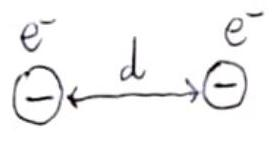
\includegraphics[width=0.5\textwidth]{2025_10_16_f02af6fa434c9f0bcc00g-02}
\end{center}

THERE is A specific ratio between\
$\rightarrow$ ELECTROSTATIC ENERGY\
$\rightarrow$ REST MASS ENERGY\
the ratio is a function of\
$\alpha$\
$\left.\begin{array}{l}\text { DIFFERENT } \\ \hbar, c, K_{B}\end{array}\right\} \begin{aligned} & \text { SAME UNIVERSE } \\ & \text { DIFFERENT UNITS }\end{aligned}$\
$\left.\begin{array}{c}\text { DIFFERENT } \\ \alpha\end{array}\right\}$ ANOTHER UNIVERSE, SIFFERENY FROM OURS

\section*{Revaew: Quantum Mech}
(1) The quantum State $\rightarrow$ (I⿴囗 POSSIBEE) TO SEFANG MEERIMINGT CALEY EVERY MGSURAALE PROPERTY OT A SYSTEM

\begin{center}
\begin{tabular}{|l|l|l|l|l|}
\hline
TAKE $\dot{x}$\operatorname{POSITION} & 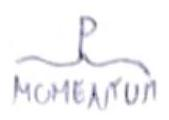
\includegraphics[width=0.5\textwidth]{2025_10_16_f02af6fa434c9f0bcc00g-03} & IF ONE IS COAPUETELY DETERMINES & $x=x_{0}$ & MSTRIBUTION $\delta\left(x-x_{0}\right)$ \\
\hline
 &  & THE OITHER ONE IS COMPEETECY UNDE TERHIVED &  & DISTRIBUTION "constant" \\
\hline
\end{tabular}
\end{center}

\begin{figure}[h]
\begin{center}
  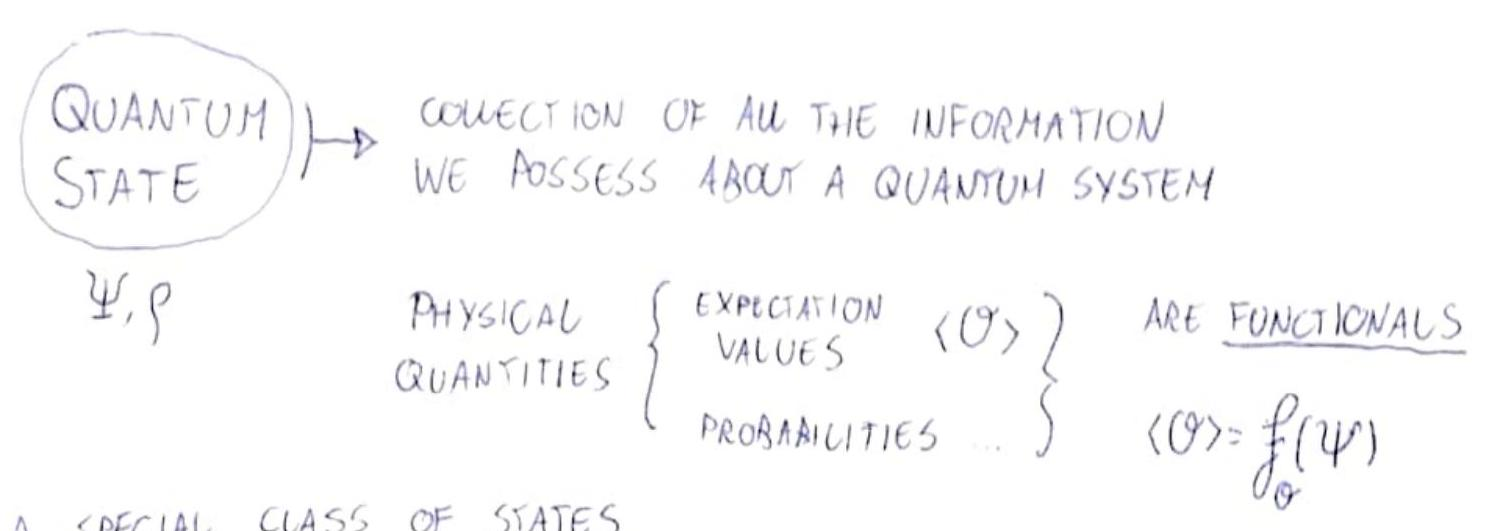
\includegraphics[width=0.5\textwidth]{2025_10_16_f02af6fa434c9f0bcc00g-03(2)}
\captionsetup{labelformat=empty}
\caption{A SPECIAL CLASS OF STATES}
\end{center}
\end{figure}

$$ \stackrel{\text { PURE }}}{\text { STATES }} \longleftrightarrow \stackrel{\text { A.K.A }}{\longleftrightarrow} \stackrel{\text { VECTOR }}{\longleftrightarrow} \frac{\text { A.K.A }}{\text { STATES }} \longleftrightarrow \text { WAVEFUNCYIONS) } $$

are "the most deterministic" states: you can not add information WITHOUY VIOLATING SOMETHING\
$|\psi\rangle$\
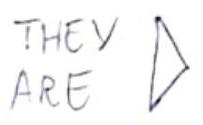
\includegraphics[width=0.5\textwidth, center]{2025_10_16_f02af6fa434c9f0bcc00g-03(1)}\
vectors of a vector space if $\left\{\begin{array}{l}|\psi\rangle+|\varphi\rangle \in \mathbb{H} \\ \lambda|\psi\rangle \in \mathbb{H}\end{array}\right.$
\rightarrow ON COMPLEX FIELD $\lambda|\psi\rangle, \lambda \in \mathbb{C}$
\rightarrow WITH A PROSUCT SCALAR HETRIC $\langle\psi \mid \varphi\rangle$
\rightarrow (CATCH) $|"psi">$ and $\lambda|"psi">$ are actoally the $\frac{\text { Same }}{\text { STATE }}$

$$ \left(\text { RUT } \lambda_{1}|\psi\rangle+\lambda_{2}|\varphi\rangle \text { ANS } \lambda_{2}|\psi\rangle+\lambda_{1}|\varphi\rangle \text { ARE NOT }\right) $$

$\mathbb{1A}$\
the Hilbert metric
$\left.\langle\varphi \mid \psi\rangle \quad \begin{array}{ll}\text { physical } & \\ = & \text { heaning }\end{array}\right\}$\n$\langle\psi \mid \varphi\rangle^{*}$

\section*{it follows that}
The probability of preparing $|"psi">$ and then measuring $|"phi">$

$$ \frac{\text { IS }}{p}=|\langle\varphi \mid \psi\rangle|^{2} \quad \frac{\text { AKA }}{\text { F/ISEUY }}
$$ 

\begin{center}
\begin{tabular}{ll}
Orthogonal & $\langle\varphi \mid \psi\rangle=0 \quad$ are $\quad$ oisting $\quad$ tashable \\
\end{tabular}
\end{center}

WHY ? B) BECAUSE IT inTRODUCES A CONCEPT OF "STATE AISTANCE"\METRIC" ?

$$ \text { EXAMPLE BURES } D_{B}("psi", \varphi)=\sqrt{2(1-\K \psi|\varphi\rangle)}
$$ 

(1B) Superposition and Interference\
input states $\left|\psi_{1}\right\rangle$ or $\left|\psi_{2}\right\rangle$, heasuring probability of output $|"phi">$
AMPUITUDES $\quad\left\langle\varphi \mid \psi_{1}\right\rangle=c_{1} \quad$ DROBABICITIES $\quad\left|\left\langle\varphi \mid \psi_{1}\right\rangle\right|^{2}=\left|c_{1}\right|^{2}=p_{1}$

$$ \left\langle\varphi \mid \psi_{2}\right\rangle=c_{2} \longrightarrow\left|\left\langle\varphi \mid \psi_{2}\right\rangle\right|^{2}=\left|c_{2}\right|^{2}=p_{2} $$

SOR $\begin{aligned} & \text { ORTHOGONAL } \\ & \text { SIMPLITY }\end{aligned} \quad \begin{aligned} & \left\langle\psi_{1} \mid \psi_{2}\right\rangle=0 \\ & \end{aligned}|+\rangle=\frac{\left|\psi_{1}\right\rangle+\left|\psi_{2}\right\rangle}{\sqrt{2}}$ IS NORMALIZES\
remainder\
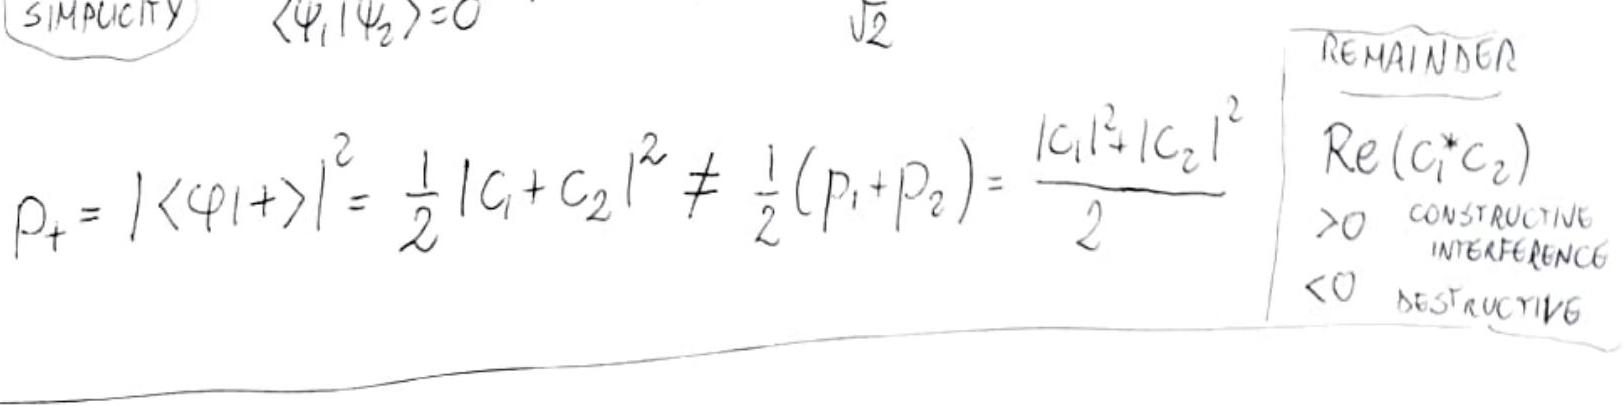
\includegraphics[width=0.5\textwidth, center]{2025_10_16_f02af6fa434c9f0bcc00g-04}\
Actually the peobability is

$$ p=\frac{|\langle\psi \mid \varphi\rangle|^{2}}{\langle\psi \mid \psi\rangle\langle\varphi \mid \varphi\rangle} \quad \leqslant \frac{\text { Physical } Q . \Leftrightarrow \begin{array}{l}\text { INVARIANT UNDER } \\ \text { 'GAUGEE TRALFFORM. }\end{array}}{\begin{array}{r}|\psi\rangle \rightarrow \lambda|\psi\rangle \text { WITH } \lambda \in \mathbb{C}(\lambda \neq 0) \\ \text { THUS WE WORK WITH NORMALIZES } \\ \text { GUANTUH STATES }\langle\psi \mid \psi\rangle=\langle\varphi \mid \varphi\rangle=1\end{array}} $$

IC Ortmonormal Bases\
FOR AU PRACTICAL purposes

$$ \operatorname{DIMENSION}(\text { If })=7^{\text {FINITE }}{ }^{\text {COUNTABLE INFINITE }}
$$ 

Why? Because 10. The lab/sample is finite size\
(2.) WE WORK AT BOUNSES EWEREY

DEFINE AN ORTHONORMAL BASIS $\left\lvert\, \begin{gathered}\text { n } \\ \uparrow\end{gathered}\right.$ BAND WIOTH

LABEL = ONE OR MORE INTEGERS\
$\begin{array}{cc}\langle n| n\left\rangle=\delta_{n, n^{\prime}}\right. & \begin{array}{c}\text { KRONECKER } \\ \text { DECTA } \\ \text { NOT SIRAC }\end{array} \\
\text { HIMSENT METRIC } & \end{array} \quad |\psi\rangle=\sum_{\substack{\mid \\ \text { GOES IN HERE }}}} C_{n}|n\rangle \quad \begin{gathered}\text { COMPLETE- } \\ \downarrow \\ \text { NESS }\end{gathered}$

\section*{1D OPERATORS}
they are ensomorphisms of ff (linear and H $\rightarrow$ H )\
NOTATION $\rightarrow \hat{A}|\psi\rangle$
WHERE $\langle\varphi \mid \psi\rangle$

$$ \begin{aligned}
& \left\langle\psi_{1}\right| \hat{A}\left|\psi_{2}\right\rangle \stackrel{\text { def }}{=}\left(\left|\psi_{1}\right\rangle, \hat{A}\left|\psi_{2}\right\rangle\right)_{\text {APAIES TO THE RIGHT }} \\
& =\left(\begin{array}{c}\text { definition of } \\ \text { HERMITIAN } \\ \text { CONGUEATE }\end{array}\right) \quad \left(\hat{A}^{+}\left|\psi_{1}\right\rangle,\left|\psi_{2}\right\rangle\right)=\left(\begin{array}{c}\text { HIL BERY } \\ \text { SCALAR } \\ \text { PRODET } \\ \text { PROPERTY }\end{array}\right) \quad \left(\left|\psi_{2}\right\rangle, \hat{A}^{+}\left|\psi_{1}\right\rangle\right)^{*} \\
& =\left(\left\langle\psi_{2}\right| \hat{A}^{+}\left|\psi_{1}\right\rangle\right)^{*}
\end{aligned} $$

(2.) Observables & heasurement\
an observable is a hecmitian operator $\theta=\theta^{+}$\
OR MORE PRECISELY $\langle\psi| \theta|\varphi\rangle=(|\psi\rangle, \theta|\varphi\rangle)=(\theta|\psi\rangle,\left|\varphi\right\rangle)=\langle\varphi| \theta|\psi\rangle^{*}$

$$ \begin{aligned}
& \theta=\theta^{+} \\
& \text {SPECTRAL } \\ & \text { THEOREM }
\end{aligned}\left\{\begin{array}{ccc}\theta \text { CAN BE DIAGONALIZED } & \\
& \& \\
& \text { ITS EIGENBASIS IS ORTHOGONAL } & \left(\begin{array}{c}\text { AT LEAST ONE } \\ \text { H EIGENGASIS } \\ \text { I SORHOGONAL }\end{array}\right) \\
& \text { EIGENVALUES ARE } & \text { REAL } \
\end{array}\right. $$

$$ G=U D U^{+} \underset{\text { DIAGONAC & REAL }}{U U^{+}=U^{+} U=\mathbb{1}} \quad U=\sum_{\substack{j \\ \sum_{\text {EIGENVALUES }}}}} \eta_{j} \mid J \times\left\langle\varphi_{j}\right| \quad\left(\eta_{1}=\eta_{j}^{*}\right) $$

$2A$ The (hard) measurement process\
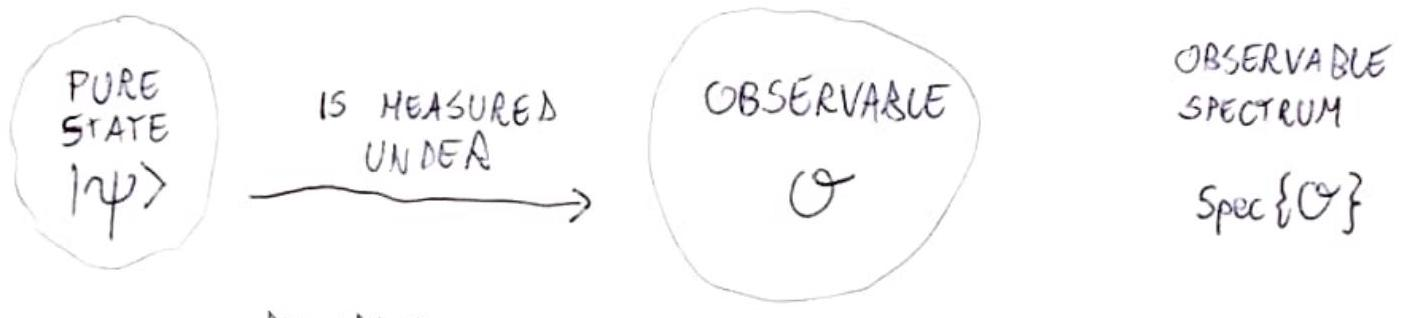
\includegraphics[width=0.5\textwidth, center]{2025_10_16_f02af6fa434c9f0bcc00g-06}

$$ \begin{gathered}
\text { For EVERY OUTCOME } \\ \lambda \in \operatorname{SPCC}\{\theta\} \\ \Downarrow \\ \Pi_{\lambda} \quad \begin{array}{c}\text { PROSECTOR OVER } \\ \text { THE EIGENSPACE }\end{array} \\ \theta \Pi_{\lambda}|\phi\rangle=\Pi_{\lambda}|\phi\rangle \lambda \\ {\left[\Pi_{\lambda}, \theta\right]=0} \\ \Pi_{\lambda}=\Pi_{\lambda}^{2}=\Pi_{\lambda}^{\dagger}
\end{gathered} $$

$$ \begin{aligned}
& \left.\| \psi_{\lambda}^{\prime}\right\rangle=\frac{\pi_{\lambda}|\psi\rangle}{\sqrt{\langle\psi| \pi_{\lambda}|\psi\rangle}}
\end{aligned} $$

THIS PROCESS BREAKS TIME REVERSAL (it is FINE BECAUSE it is AN EFFECTIVE PICTURE)

$$ \langle\psi\rangle=\sum_{\lambda}^{1} \lambda p_{\lambda}=\langle\psi|\left(\Sigma \lambda \Pi_{\lambda}\right)|\psi\rangle=\langle\psi| \circlearrowleft|\psi\rangle $$

$$ \Delta \theta^{2}=\left\langle\theta^{2}\right\rangle-\langle\theta\rangle^{2} $$

$=\left\langle\left(\theta-\left.\langle\theta\rangle\right|^{2}\right\rangle

2B operators & observables so not commute

\section*{i[A, B]=C}
$\Delta A \Delta B \geqslant \frac{1}{2}|\langle i[A, B]\rangle| \begin{aligned} & \text { Heisenserg } \\ & \text { uncertanty principle }\end{aligned}$

\section*{in practice}
\begin{center}
\begin{tabular}{|l|l|l|l|l|}
\hline measure A & A 15 DETERMINES & MEASURE B & B IS DETERMINES & A IS NO HORE DETERMINED \\
\hline HEISENBERG IS NOT ALWAYS A HARD BOWND & $\Delta p \Delta x \geqslant$ & $\frac{\hbar}{2}$ & HARD BOUND & $\Delta p \rightarrow 0$ MEANS $\Delta x \rightarrow \infty$ \\
\hline
\end{tabular}
\end{center}

\section*{BUT CONSIDER}
$|0\rangle=\binom{1}{0}$

$$ \sigma^{z}=\binom{1}{-1} \quad \sigma^{x}=\left(\begin{array}{ll}0 & 1 \\ 1 & 0\end{array}\right) \quad \sigma^{y}=\left(\begin{array}{ll}-i & \\ i & \end{array}\right) $$

$|1\rangle=\binom{0}{1}$

$$ \Delta \sigma_{0}^{z} \Delta \sigma_{0}^{x} \geqslant \frac{1}{2}\left|\left\langle\sigma^{y}\right\rangle_{0}\right| $$

$\Delta \sigma_{0}^{z}=\langle 0|\left(\sigma^{z}-\langle 0| \sigma^{z}|0\rangle\right)^{2}|0\rangle=\langle 0|\left(\sigma^{z}-1\right)^{2}|0\rangle=\sqrt{0}\left(\begin{array}{ll}0 & 0 \\ 0 & 4\end{array}\right)\binom{1}{0}=0$
$\Delta \sigma_{0}^{x}=\langle 0|\left(\sigma^{x}-\langle 0| \sigma^{x}|0\rangle\right)^{2}|0\rangle=\langle 0| \sigma^{x^{2}}|0\rangle=\langle 0 \mid 0\rangle=1$
$\left\langle\sigma_{0}^{y}\right\rangle_{0}=\frac{10}{10}\binom{-i}{i}\binom{1}{0}=0$
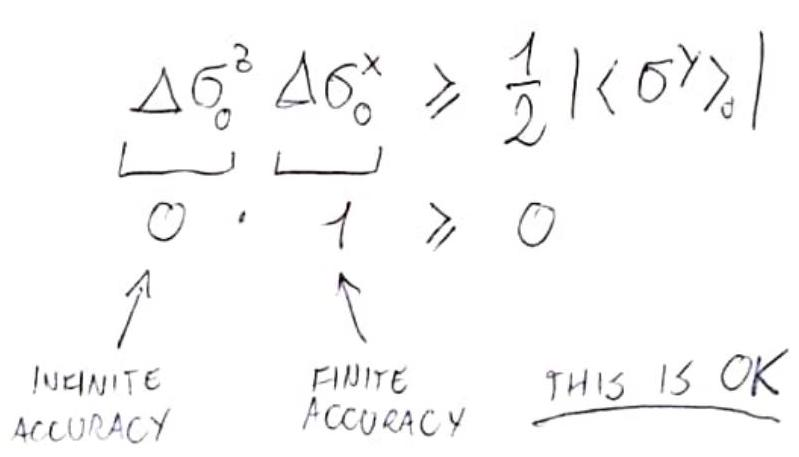
\includegraphics[width=0.5\textwidth, center]{2025_10_16_f02af6fa434c9f0bcc00g-07}

$$ 0 \geqslant 0 $$

WEU, WHATEVER\
NOT REACY HARD BOUND\
that's one reason why Q-IN.O MAKES SENSE\[0pt]
[2C] Physical transformations of a closes quantum system\
IF A SYSTEM IS CLOSED

$$ \left.\left.|"psi"> \rightarrow\left|\psi^{\prime}\right\rangle={ }^{*} I(|\psi\rangle)=|T| \psi\right\rangle\right
angle $$

(1) IT STAYS DETERMINISTIC\
(2) If PRESERVES TOTAL PROBALIKY

$$ \langle T("psi")| \mathbb{1}|T("psi")\rangle=\langle\psi| \mathbb{1}|\psi\rangle=1 $$

under physical transformations

$$ (T \psi, T \psi)_{H}=(\psi, \psi)_{H} \quad \forall \psi\left[\begin{array}{c}\text { THEREE ARE ONCY TWO } \\ \text { POSSIBICITIES }\end{array}\right. $$

\section*{T ANTI-UNITARY}
$(T \psi, T \varphi)=(\psi, \varphi)^{*} \quad \forall \psi \varphi$
PROBLEM CANNOT CONTINUUJSLY connect with trivital trafo $\mathbb{1}_{.}$ MAOSSIBLE TO ACHIEVE WITH increhental changes

$$ \binom{\text { STIU USEFUL AS A }}{\text { SYMHETRY }}
$$ 

T UNITARY\
$(T \psi, T \varphi)=(\psi, \varphi) \quad \forall \psi, \varphi$
$1_{\text {THIS IS THE COMMON CASE: }}$ CONTINUOUSLY CONNECTES TO 11 SO TIME EVOLUTION OPERATORS ARE OF THIS CCASS

$$ \left|\psi\left(t^{\prime}>t\right)\right\rangle=U\left(t, t^{\prime}\right)|\psi(t)\rangle $$

\begin{itemize}
  \item change of reference frame can be both untary and anti-unitary\
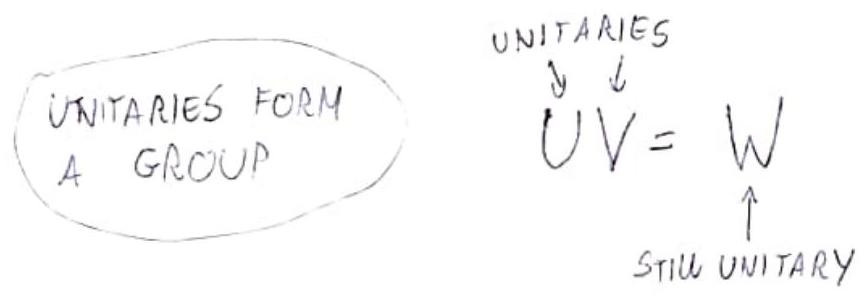
\includegraphics[width=0.5\textwidth, center]{2025_10_16_f02af6fa434c9f0bcc00g-08(1)}\
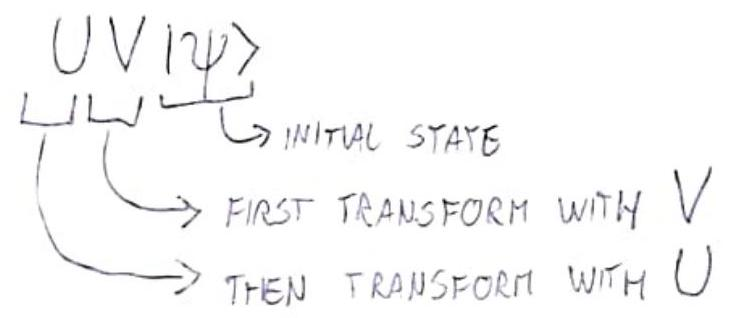
\includegraphics[width=0.5\textwidth, center]{2025_10_16_f02af6fa434c9f0bcc00g-08(2)}
\end{itemize}

\begin{figure}[h]
\begin{center}
\captionsetup{labelformat=empty}
\caption{hanes sense: stacking hultiple AHYSICA OPS IS STILE A PUYSICAL Op.}
  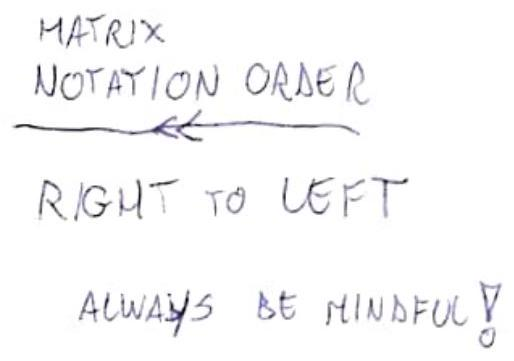
\includegraphics[width=0.5\textwidth]{2025_10_16_f02af6fa434c9f0bcc00g-08}
\end{center}
\end{figure}

(3) Time Evolution

INITIAC CONDITIONS

CLOSES SYSTEM EVO\
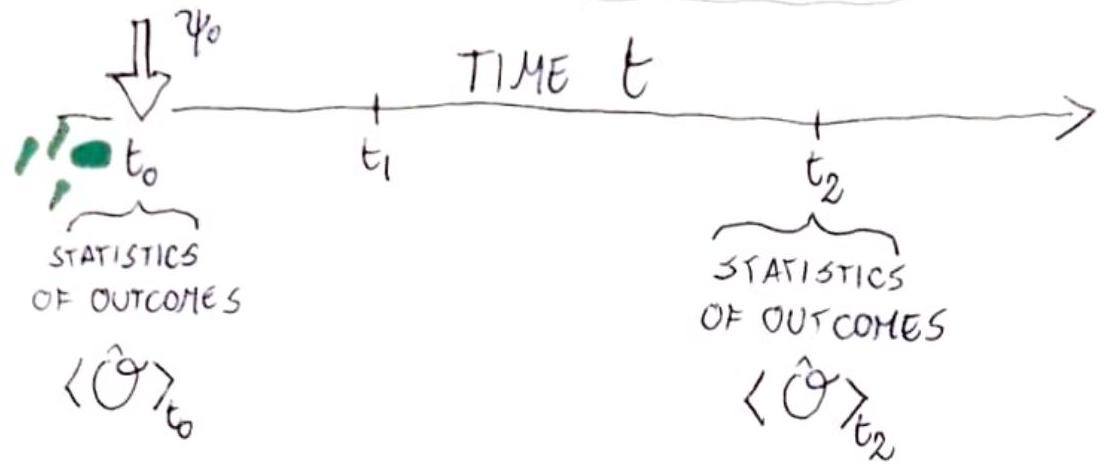
\includegraphics[width=0.5\textwidth, center]{2025_10_16_f02af6fa434c9f0bcc00g-09}

3A. Schrödinger PICTURE - Evolving Stotes

$$ i \hbar \frac{d}{d t}|\psi\rangle=\hat{H}|\psi\rangle \quad \begin{gathered}\text { SCHIÖSINGER'S } \\ \text { EQUATION }\end{gathered} \quad \begin{aligned}
& \text { WHERE } \\ & H=H^{+} \end{aligned} $$

holss for EVERY quantum system evo that is
(a) PHYSICAL
(2) $\operatorname{closes}$
(3) FIRST-ORSER SIFFERENTIAL IN TIME\
(in a way, schrósinger can be relativistic if $H$ is relativistic)

\section*{formal Solutions $H$ is $t$ insepensent}
Ao Diagonalize $H=\sum \varepsilon_{s}\|\varepsilon_{s} \times \varepsilon_{s}\| \quad\binom{\text { so THAT }}{H\left|\varepsilon_{s}\right\rangle=\left|\varepsilon_{s}\right\rangle \varepsilon_{s}}$

$$ \left|\varepsilon_{j}\right\rangle \xrightarrow{E V O C U T I O N} e^{-i \varepsilon_{j} t / \hbar}\left|\varepsilon_{j}\right\rangle $$

B. Expand any intital state $\left|\psi_{0}\right\rangle$ in the eigenbasis

$$ \begin{aligned}
& \left\langle\varepsilon_{j} \mid \psi_{0}\right\rangle=c_{j} \\
& \left|\psi_{0}\right\rangle=\sum_{1} c_{j}\|\varepsilon_{j}\rangle \xrightarrow{\text { EVOLVE }}|\psi(t)\rangle=\sum_{1}^{1}\left|\varepsilon_{j}\right\rangle c_{j} e^{-i \varepsilon_{j} t / \hbar}
\end{aligned} $$

(BANDWIJTH!),\
c. formal expression with the matrix exponential

$$ \begin{aligned}
|\psi(t)\rangle & =\underbrace{\left(\sum_{1}\left|\varepsilon_{j}\right\rangle e^{-i \varepsilon_{j} t / \hbar}\left\langle\varepsilon_{j}\right|\right)\left|\psi_{0}\right\rangle}_{\substack{\text { ANS TAS IS INSEES UNTARY } \\ \text { AND ADATIVE } U\left(t_{2}\right) U\left(t_{1}\right)=U\left(t_{1}+t_{2}\right)}} \\
\exp (-i H(t / \hbar) & \left|\psi_{0}\right\rangle
\end{aligned} $$

DONT FORGET THAT $\exp (A)=1+A+\frac{A^{2}}{2}+\frac{A^{3}}{6}+\ldots=\sum_{j=0}^{\infty} \frac{A^{j}}{j!}$ BUT ALSO $\exp \left(V A V^{+}\right)=V \exp (A) V^{+}$SO ORTENTIMES\
(e) DIAGONALIEE\
(2) examentate the eigenvalues

3B. Heisemberg PICTURE - Evolving OPS

$$ \begin{array}{rlr}
\langle\theta\rangle_{t}=\langle\psi| \theta|\psi\rangle_{t}=\left\langle\psi_{0}\right| \underbrace{+}_{\vec{\theta}(t)}(t) \theta(t)\|\psi_{0}\rangle & \dot{U}(t)=\frac{d}{d t}\left(e^{-i H t / \hbar}\right) \\
\frac{d}{d t} \tilde{\theta}(t)=\dot{U}^{+}(t) \theta U(t)+U^{+}(t) \theta \dot{U}(t) & \left(-\frac{i}{\hbar} H\right) U(t) \\
& =+\frac{i}{\hbar} H U^{+} \theta U-\frac{i}{\hbar} U^{+} \theta U M & {[H, U]=0} \\
\dot{\omega} & =\frac{i}{\hbar}[H, \tilde{\theta}] \quad\left(+U^{+} \dot{\theta} U\right)
\end{array} $$

\section*{3C EXAMPLE: DRIVEN 2-LEVEL SYSTEM AND TRANSITIONS}
\begin{center}
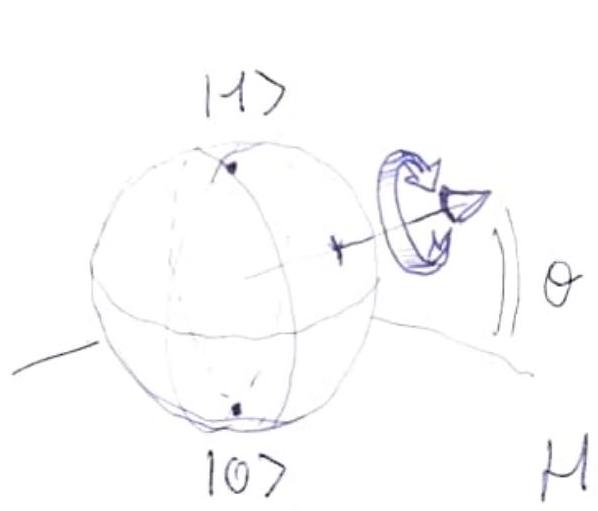
\includegraphics[width=0.5\textwidth]{2025_10_16_f02af6fa434c9f0bcc00g-11}
\end{center}

$$ \begin{aligned}
& \left|\psi_{0}\right\rangle=0 \\
& \left\lvert\, \begin{array}{l}
\mid=\hbar\left(\Omega \sigma^{x}+\Delta \sigma^{z}\right) \\ \binom{\text { RABI }}{\text { REQ. }} \quad \text { (DETUNING) } \leftarrow \text { WE WIU SEE } \\ \text { WHY THIS } \\ \text { IS } \\ \text { THE CASE }\end{array}\right.
\end{aligned} $$

$$ H=\hbar \Omega\left(\begin{array}{ll}0 & 1 \\ 1 & 0\end{array}\right)+\hbar \Delta\left(\begin{array}{cc}1 & 0 \\ 0 & -1\end{array}\right)=\hbar\left(\begin{array}{cc}\Delta & \Omega \\ \Omega & -\Delta\end{array}\right) $$

REWRITE $\ \widetilde{\Omega}=\sqrt{\Omega^{2}+\Delta^{2}} \quad \theta=\arctan \left(\frac{\Delta}{\Omega}\right)$

$$ \begin{aligned}
& \rightarrow \Omega=\Omega \sin \theta \quad \Delta=\tilde{\Omega} \cos \theta \\
& H=\hbar \widetilde{\Omega}(\vec{n} \cdot \overrightarrow{\vec{\sigma}}) \\ & \text { NOTICE THAT }(\vec{n} \cdot \vec{\sigma})^{2}=\mathbb{1}
\end{aligned} \vec{n}=\left(\begin{array}{c}\cos \theta \\ 0 \\ \sin \theta\end{array}\right) \quad \vec{\sigma}=\left(\begin{array}{c}\sigma^{x} \\ \sigma^{y} \\ \sigma^{z}\end{array}\right) $$

Therefore $\exp \left(-\frac{i \mu t}{\hbar}\right)=\sum_{J} \frac{(-i \tilde{\Omega} t)^{j}}{J!}(\vec{n} \cdot \hat{\vec{\sigma}})^{J}$

$$ \begin{aligned}
= & 1 \sum_{j}^{\text {ever }} \frac{(-i \tilde{\Omega} t)}{j !}+(\vec{n} \cdot \hat{\vec{\sigma}}) \sum_{j}^{\cos } \frac{(-i \Omega t)}{J!} \\
= & \mathbb{1} \cos (\tilde{\Omega} t)-i \sin (\tilde{\Omega} t)\left(\begin{array}{cc}\sin \theta & \cos \theta \\ \cos \theta & -\sin \theta\end{array}\right) \\
& \cos (\tilde{\Omega} t)\left(\begin{array}{cc}1 & 0 \\ 0 & 1\end{array}\right)-i \sin (\tilde{\Omega} t)\left(\begin{array}{cc}i \sin \theta & \cos \theta \\ \cos \theta & -i \sin \theta\end{array}\right) \\
& \left|\psi_{0}\right\rangle=0 \quad=\quad \binom{1}{0} \\
& |\psi(t)\rangle=\quad \cos (\tilde{\Omega} t)\binom{1}{0}-i \sin (\tilde{\Omega} t)\left(\begin{array}{c}i \sin \theta \\ \cos \theta\end{array}\right)
\end{aligned} $$

probability of measuring (H)

$$ |\langle 1 \mid \psi(t)\rangle|^{2}=\left|\frac{}{01}\binom{\cos \left(\tilde{\Omega}_{t}\right)-i \sin \left(\tilde{\Omega}_{t}\right) \sin \theta}{-i \sin \left(\tilde{\Omega}_{t}\right) \cos \theta}\right|^{2} $$

$$ =\sin ^{2}(\Omega t) \cos ^{2} \theta $$

\begin{center}
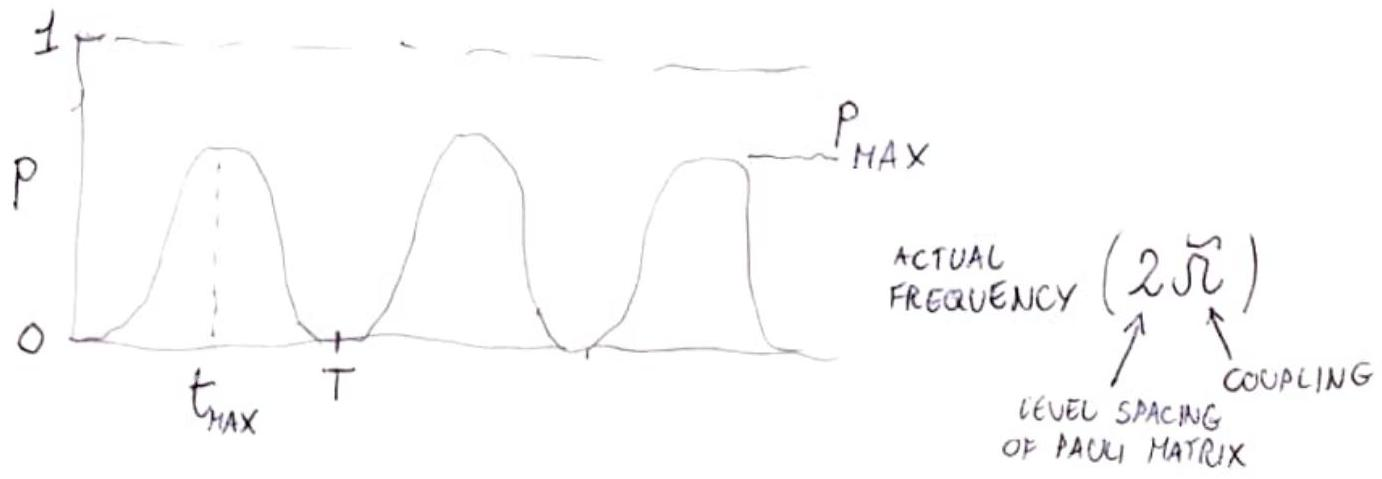
\includegraphics[width=0.5\textwidth]{2025_10_16_f02af6fa434c9f0bcc00g-12}
\end{center}

$$ t_{\text {MAX }}=\(2 J+1) \frac{\pi}{2 \dot{\Omega}}=(2 J+1) \frac{\pi}{2 \sqrt{\Omega^{2}+\Delta^{2}}} \quad T=\frac{\pi}{\Omega} $$

$\xrightarrow[\substack{\text {TRANSIGION } \\ \text { PROB. }}]{\text { MAX }} P_{\text {MAX }}=\cos ^{2} \theta=\frac{\Omega^{2}}{\Omega^{2}+\Delta^{2}}=\left(1-\frac{\Delta^{2}}{\Omega^{2}+\Delta^{2}}\right) $
$\Downarrow$
qualitative lesson:\nTo have high transition\
YOU NEES $\triangle \ll \Omega$
(mportant later)

% Lecture file created by Gemini
% Class: Quantum Information With Atoms and Photons
% Professor: Pietro Silvi
% Date: 2025-10-16
\lecture{2}{Degenerate Perturbation Theory}{2025-10-16}

% --- Start writing here ---
\begin{enumerate}
  \setcounter{enumi}{3} 
  \item Perturbation Theory (the indefendent)\
done in a way that is useful\
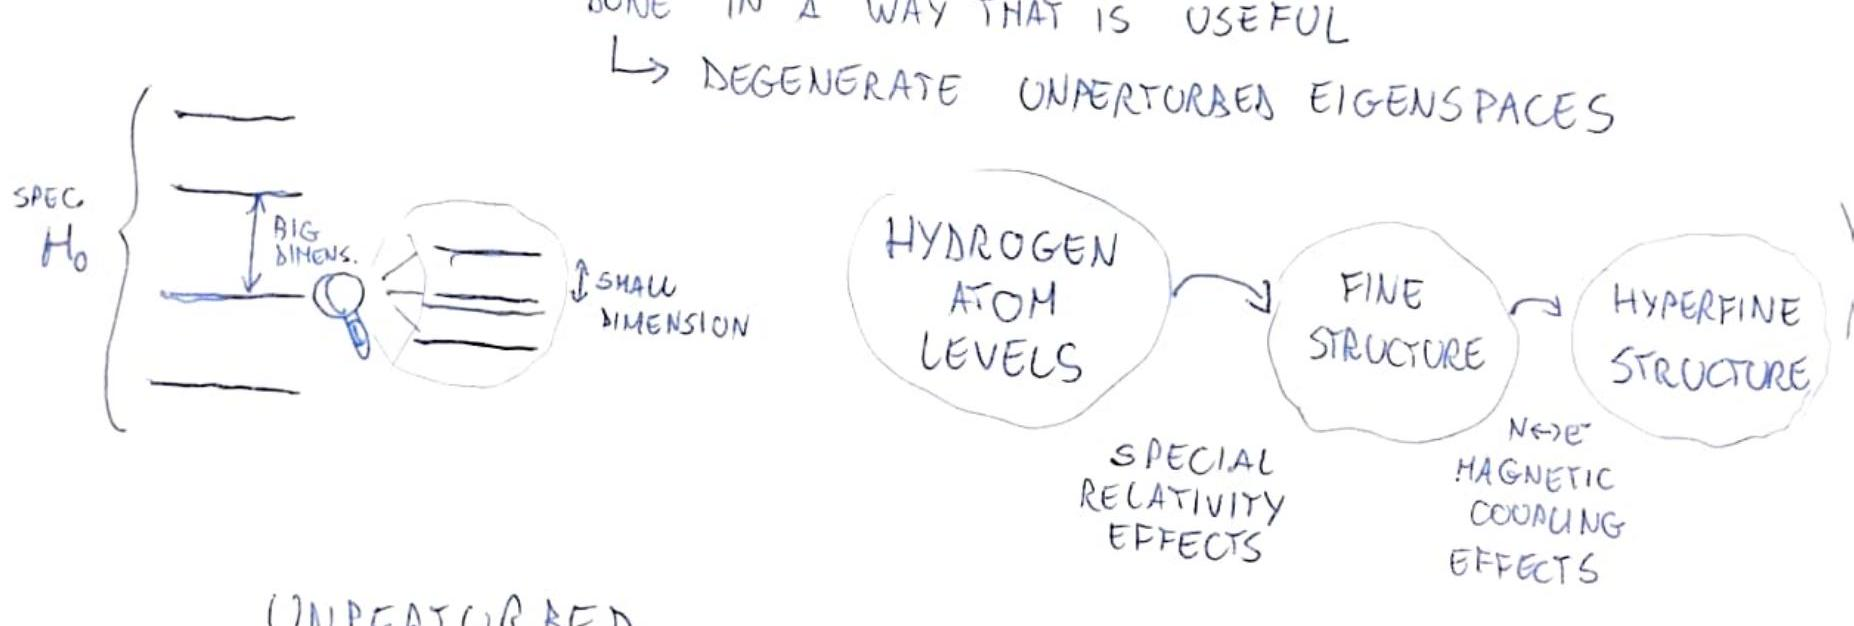
\includegraphics[max width=\textwidth, center]{2025_10_16_f6b2ddb567eefef2c7a2g-1(1)}
\end{enumerate}

UNPERTURBED

\section*{hamiltonian}
$H_{0}\left|\varepsilon^{(0)}, J\right\rangle=\varepsilon^{(0)}\left|\varepsilon^{(0)}, J\right\rangle$\
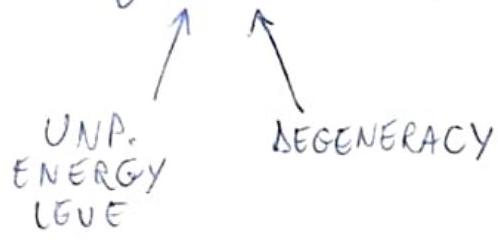
\includegraphics[max width=\textwidth, center]{2025_10_16_f6b2ddb567eefef2c7a2g-1}

EXAMPLE

$$
\left(\begin{array}{rll}
\varepsilon_{0} & & \\
& \varepsilon_{0} & \\
& & \rightarrow \\
& & \mid \varepsilon_{1}
\end{array}\right) \xrightarrow{\rightarrow}\left|\varepsilon_{0}, 1\right\rangle=\left(\begin{array}{l}
1 \\ 0 \\ 0
\end{array}\right)=\left(\begin{array}{l}
0 \\ 1 \\ 0
\end{array}\right)=\left(\begin{array}{l}
0 \\ 0 \\ 1
\end{array}\right)
$$

$\widetilde{\varepsilon}_{n}=\varepsilon_{n}^{(0)}+\lambda \varepsilon_{n}^{(1)}+\lambda^{2} \varepsilon_{n}^{(2)}+...$\
$\left|\tilde{\varepsilon}_{n}\right\rangle=\left|\varepsilon_{n}^{(0)}\right\rangle+\lambda\left|\varepsilon_{n}^{(1)}\right\rangle+\cdots$ Also WITH $J$
$\left(H_{0}+\lambda V\right)\left(\left|\varepsilon^{(0)}, J\right\rangle+\lambda\left|\varepsilon^{(1)}, J^{1}\right\rangle+\ldots\right)=\left(\varepsilon^{(0)}+\lambda \varepsilon^{(1)}+\ldots\right)\left(\left|\varepsilon^{(1)}, J\right\rangle+\lambda \mid \varepsilon^{(1)}, J\right.$\
ORDER $1=\lambda^{\circ}$\n$H_{0}\left|\varepsilon^{(0)}, J\right\rangle=\varepsilon^{(0)}\left|\varepsilon^{(0)}, J\right\rangle$ well, AT LEAST IT IS CONSISTENT

ORSER $\lambda=\lambda^{1}$\n$V\left|\varepsilon^{(0)}, J\right\rangle+H_{0}\left|\varepsilon^{(1)}, J^{\prime}\right\rangle=\varepsilon^{(1)}\left|\varepsilon^{(0)}, J\right\rangle+\varepsilon^{(0)}\left|\varepsilon^{(1)}, J^{\prime}\right\rangle$

$$
\Pi=\Pi^{+}=\Pi^{2}
$$

$\left.\begin{array}{l}\text { I now DEFINE THE PROSECYOR } \\ \text { ONTO THE } \varepsilon^{(0)} \text { EIGENSPACE OF } H_{0}\end{array}\right\} \quad \Pi_{\varepsilon_{0}}=\sum_{\zeta}\left|\varepsilon^{(0)}, J\right\rangle\left\langle\varepsilon^{(0)}, J\right|$

$$
\prod_{\varepsilon_{0}} H_{0}=H \prod_{0}=\varepsilon^{(0)} \Pi \quad \ldots \text { AND I HULTIPLY LEFT. } 
$$

$\Pi_{\varepsilon_{0}} V\left|\varepsilon^{(0)}, J\right\rangle+\underbrace{\ldots}_{\varepsilon_{0}} H\left|\varepsilon^{(1)}, J^{\prime}\right\rangle=\varepsilon^{(1)} \Pi_{\varepsilon_{0}}\left|\varepsilon^{(0)}, J\right\rangle+\varepsilon^{(0)} \Pi_{\varepsilon_{0}}\left|\varepsilon^{(0)}, J^{\prime}\right\rangle$

$$
\varepsilon^{(0)} \Pi_{\varepsilon^{(0)}}\left|\varepsilon^{(+)}, J^{\prime}\right\rangle
$$

$\left|\varepsilon^{(0)}, J\right\rangle=\pi_{\varepsilon^{(0)}}\left|\varepsilon^{(0)}, J\right\rangle$

$$
\prod_{\varepsilon(0)}\left|\varepsilon^{(0)}, j\right\rangle=\left|\varepsilon^{(0)}, j\right\rangle
$$

$$
(\underbrace{\Pi_{\varepsilon_{0}} \vee \Pi_{\varepsilon_{0}}})\left|\varepsilon^{(0)}, J\right\rangle=\varepsilon^{(1)}\left|\varepsilon^{(0)}, J\right\rangle \quad \forall J
$$

$\Rightarrow \underbrace{(\pi V \pi)^{+}=\pi^{+} V^{+} \pi^{+}=\pi V \pi}_{\text {HERMITIAN }}$\nEigenvalue Equation
$\rightarrow$ IT TEUS US HOW THE SEGENERACY IS REMOVES AND\nHOW THE RESOLVED STATES LOOK LIKE
Notice $\rightarrow$ the resolves states are (NOT) a correction from an arbitrary $|\varepsilon, j\rangle$ (see example later)

EXCERCISE
$\lambda H_{\varepsilon_{i}^{(1)}}^{(1)}\left|\varepsilon^{(0)}, J\right\rangle=\lambda \varepsilon^{(1)}\left|\varepsilon^{(0)}, J\right\rangle$
where $\lambda M_{\varepsilon_{0}}^{(1)}=\lambda\left(\Pi_{\varepsilon^{(0)}} \vee \Pi_{\varepsilon^{(0)}}\right)$

CONTRACT * WITH

$$
\left\langle\varepsilon_{n}^{(0)}, J\right| \text { AND }
$$
LEARN SOMETHING ABOUT $\left|\varepsilon^{(1)}, J\right\rangle$

GA HIGHER ORDERS OF DEG-REMOVING HAMICTONIANS $L$ USUALLY THE COWEST NONZERO ORDER COUNTS

NON-DEG

$$
\begin{aligned}
& H_{0}^{(1)}=\Pi_{\varepsilon_{0}} V \Pi_{\varepsilon_{0}} \\
& \varepsilon^{(1)}=\left\langle\varepsilon_{0}\right| V\left|\varepsilon_{0}\right\rangle \\
& H_{\varepsilon_{0}}^{(2)}=\Pi_{\varepsilon_{0}} \vee R_{\varepsilon_{0}} \vee \Pi_{\varepsilon_{0}} \\
& \Leftrightarrow \varepsilon^{(2)}=\sum_{\varepsilon_{n} \neq \varepsilon_{0}} \frac{\left|\left\langle\varepsilon_{n}\right| V\left|\varepsilon_{0}\right\rangle\right|^{2}}{\varepsilon_{n}^{(0)}-\varepsilon_{n}^{(0)}} \\
& =\left\langle\varepsilon_{0}\right| V \underbrace{\left(\sum_{\varepsilon_{n} \varepsilon_{0}} \frac{\left|\varepsilon_{n} \times \varepsilon_{n}\right|}{\varepsilon_{0}^{(0)}-\varepsilon_{n}^{(0)}}\right)}_{\text {MOORE-PENROSE }} V\left|\varepsilon_{0}\right\rangle \\
& \text { PSEUDOINVERSE } \\
& \text { (INVERY ONCY THE) } \\
& \downarrow \\
& R_{\varepsilon_{0}}=\left(\begin{array}{ccl}
0 & & \\
& \frac{1}{\varepsilon_{0}-\varepsilon_{1}} & \\
& & \frac{1}{\varepsilon_{0}-\varepsilon_{i}}
\end{array}\right) \\
& A=\left(\begin{array}{lll}0 & & \\ & 1 & \\ & & 2\end{array}\right) \quad A^{\prime \prime \prime}=\left(\begin{array}{lll}0 & & \\ & 1 & \\ & & 1 / 2\end{array}\right) \\
& \varepsilon^{(2)}=\left\langle\varepsilon_{0}\right| V\left(\varepsilon_{0}^{(0)} \mathbb{1}-H_{0}\right)^{-1} V \mid \varepsilon \\
& H_{\varepsilon_{0}}^{(3)}=\Pi_{\varepsilon_{0}} V R_{\varepsilon_{0}} V R_{\varepsilon_{0}} V \Pi_{\varepsilon_{0}}-\Pi_{\varepsilon_{0}} V \Pi_{\varepsilon_{0}} V R_{\varepsilon_{0}}^{2} V \Pi_{\varepsilon_{0}} \\
& H_{\varepsilon_{0}}^{(4)}=\Pi_{\varepsilon_{0}} V R_{\varepsilon_{0}} V R_{\varepsilon_{0}} V R_{\varepsilon_{0}} V \Pi_{\varepsilon_{0}}-\Pi_{\varepsilon_{0}} V R_{\varepsilon_{0}}^{2} V \Pi_{\varepsilon_{0}} V R_{\varepsilon_{0}} V \Pi_{\varepsilon_{0}} \\
& -\pi \vee \pi \vee R \vee R^{2} \vee \pi-\pi \vee \pi \vee R^{2} \vee R V \pi \\
& +\pi V \pi V \pi V R^{3} V \pi
\end{aligned}
$$

(5) nonsense

EXERCISE THE LAMBDA SYSTEM (USEEVI FOR

$$
\frac{\hbar}{|0\rangle} \frac{|e\rangle}{|1\rangle}
$$

$$
|0\rangle=\left(\begin{array}{l}
1 \\ 0 \\ 0
\end{array}\right) \quad |e\rangle=\left(\begin{array}{l}
0 \\ 1 \\ 0
\end{array}\right) \quad |1\rangle=\left(\begin{array}{l}
0 \\ 0 \\ 1
\end{array}\right)
$$

$$
H_{0}=\left(\begin{array}{ccc}
0 & & \\ & +\Delta & \\ & & 0
\end{array}\right)
$$

$$
V=\left(\begin{array}{ccc}
0 & \Omega & \\ \Omega & 0 & \Omega \\ & \Omega & 0
\end{array}\right)=\Omega\left(\begin{array}{ll}1 & 1 \\ 1 & 1\end{array}\right)
$$

UN PERTURBED
GAMILTONIAN

$$
\left.\left.\begin{array}{lll}\Pi_{0}=\left(\begin{array}{ll}1 & \\ 0 & 1 \\ & 1\end{array}\right) & R_{0}=\left(\begin{array}{cc}0 & \\ -\frac{1}{\Delta} & \\ & \\ \Pi_{\Delta}=\left(\begin{array}{ll}0 & \\ 1\end{array}\right) & \end{array}\right. & H_{0}^{(1)}=0 \\ & 0
\end{array}\right)\left(\begin{array}{cc}\frac{1}{\Delta} & \\ & 0 \\ & \\ & +\frac{1}{\Delta}\end{array}\right)\right)\left(H_{\Delta}^{(1)}=0
$$

$H_{0}^{(2)}=\Pi_{0} \vee R_{0} \vee \Pi_{0}=\frac{\Omega^{2}}{\Delta}\left(\begin{array}{ll}1 & 0 \\ 1 & 1
\end{array}\right)\left(\begin{array}{ll}0 & 1 \\ 1 & 1 \\ 1 & 0
\end{array}\right)\left(\begin{array}{ll}0 & \\ 1 & 0
\end{array}\right)\left(\begin{array}{ll}1 & 1 \\ 1 & 1\end{array}\right)\left(\begin{array}{ll}1 & \\ 0 & 1
\end{array}\right)=$

$$
\Delta\left(t+\frac{2 \Omega^{2}}{\Delta^{2}}\right)=-\frac{\Omega^{2}}{\Delta}\left(\begin{array}{ll}1 & 1 \\ 1 & 0 \\ 1 & 1\end{array}\right)
$$

\begin{center}
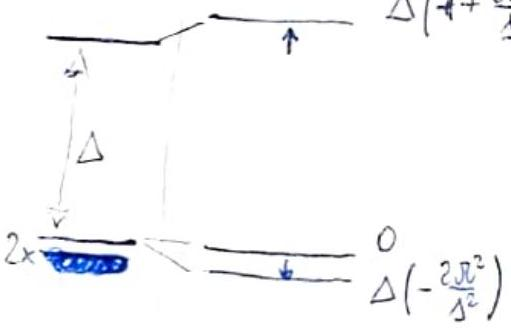
\includegraphics[width=0.5\textwidth]{2025_10_16_f6b2ddb567eefef2c7a2g-4}
\end{center}

$$
\begin{aligned}
& \text { DARH } \\
& \text { STAT } \\
& \left.\frac{2 \Omega^{2}}{\Delta}\right)
\end{aligned}
$$

$$
\begin{aligned}
& \frac{|0\rangle+|1\rangle}{\sqrt{2}} \leadsto \varepsilon^{(2)}=-\frac{2 \Omega^{2}}{\Delta} \\
& \frac{|0\rangle-|1\rangle}{\sqrt{2}} \leadsto \varepsilon^{(2)}=0 \text { DARK }
\end{aligned}
$$

$H_{2}^{(2)}=\ldots .=|e \times e|\left(+\frac{2 \Omega^{2}}{\Delta}\right) \quad \varepsilon_{e}^{(0)}+\varepsilon_{e}^{(2)}=\Delta+\frac{2 \Omega^{2}}{\Delta}$\n11)\
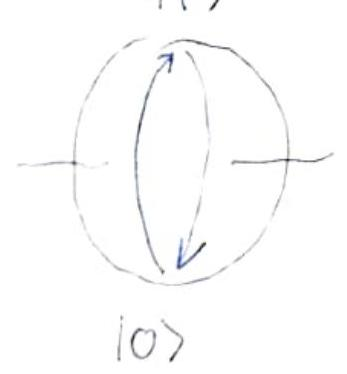
\includegraphics[width=0.5\textwidth, center]{2025_10_16_f6b2ddb567eefef2c7a2g-4(1)}

\section*{FUL RABI}
$$
=\Delta\left(1+\frac{2 \Omega^{2}}{\Delta^{2}}\right)
$$

frequency $\left|\left(0-\frac{2 \Omega^{2}}{\Delta}\right)\right|=\frac{2 \Omega^{2}}{\Delta}=\Delta\left(\frac{2 \Omega^{2}}{\Delta^{2}}\right) \ll \Delta$
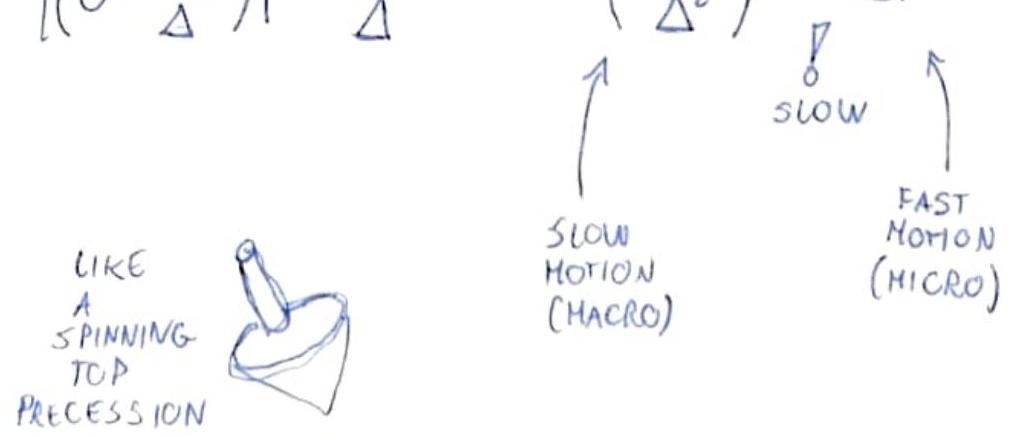
\includegraphics[width=0.5\textwidth, center]{2025_10_16_f6b2ddb567eefef2c7a2g-4(2)}

\section*{SAME Problem BUT (NO) PERTURBATION tHEORY}
$\hbar=1$

$$
\begin{array}{ll}
H_{0}=\left(\begin{array}{ccc}
0 & & \\ & +\Delta & \\ & & 0
\end{array}\right) \quad V=\left(\begin{array}{ccc}
0 & \Omega & \\ \Omega & 0 & \Omega \\ & \Omega & 0
\end{array}\right) & \text { EXACT } \\ H_{\text {TOT }}=H_{0}+V=\Delta\left(\begin{array}{ccc}
0 & \eta & \\ \eta & 1 & \eta \\ & \eta & 0
\end{array}\right) \quad \text { WITH } \quad \eta=\frac{\Omega}{\Delta} & \text { SHALU } \\ \text { PARAMETER } 
\end{array}
$$

$\left|\begin{array}{ccc}-\lambda & \eta & \\ \eta & 1-\lambda & \eta \\ & \eta & -\lambda\end{array}\right|=P(\lambda)=\lambda^{2}(1-\lambda)+2 \lambda \eta^{2}=-\lambda\left(\lambda^{2}-\lambda-2 \eta^{2}\right)$

$$
P(\lambda)=0 \rightarrow \lambda=\frac{1}{2}\left(1 \pm \sqrt{1+8 \eta^{2}}
$$

$P(\lambda)=0 \rightarrow \lambda={ }_{0}$\n$\Delta \sim \frac{1}{\uparrow} \Delta\left(\frac{1}{2}+\frac{1}{2} \sqrt{1+8 \frac{\Omega^{2}}{\Delta^{2}}}\right) \geqslant \Delta\left(\frac{1}{2}+\frac{1}{2}\left(1+4 \frac{\Omega^{2}}{\Delta^{2}}\right)\right)$\n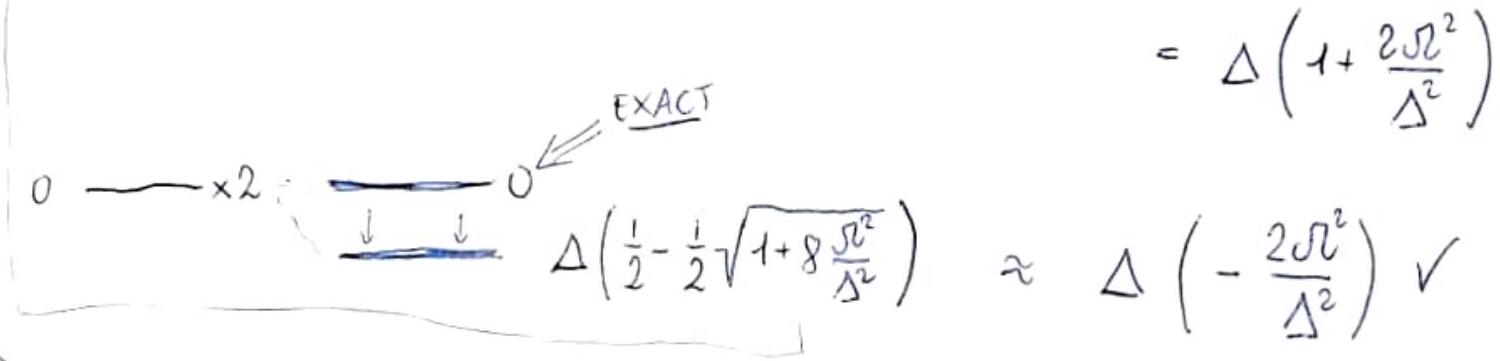
\includegraphics[width=0.5\textwidth, center]{2025_10_16_f6b2ddb567eefef2c7a2g-5(1)}\
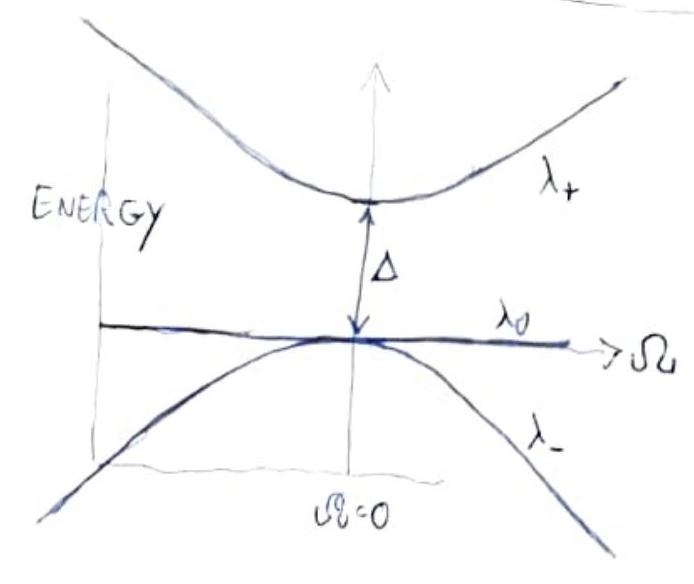
\includegraphics[width=0.5\textwidth, center]{2025_10_16_f6b2ddb567eefef2c7a2g-5}

Secular Motion

Microhotion $\mu^{\mu^{m} \eta_{\eta}}$\nsee marco's lecture
$\sim$ LIKE $A$ RABI $\sigma^{*}$\
$|0\rangle{ }^{\curvearrowleft}|1\rangle$
EREQUENCY $\left|0-\frac{2 \Omega^{2}}{\Delta}\right|=\frac{2 \Omega^{2}}{\Delta}$\nDERIOD $\frac{\pi \Delta}{\Omega^{2}}$ (slow)
WIGGLES OF AOPULATION OF $|e\rangle$

FREQUENCY $\sim \Delta$
PERIOD $\frac{2 \pi}{\Delta}$ (FAST)
5. Time-Orderes Exponential

$$
\begin{aligned}
&i \frac{d}{d t}|\psi(t)\rangle =H(t)|\psi(t)\rangle \\
&i \frac{d}{d t} U\left(t, t_{0}\right)|\psi \phi_{0}\rangle =H(t) U\left(t, t_{0}\right)|\psi_{0}\rangle
\end{aligned}
$$

$|\psi(t)\rangle=U\left(t, t_{0}\right)|\psi_{0}\rangle \quad$ WITH

$$
\underset{\substack{\text { ASSITIVITY } \ U\left(t_{2}, t_{1}
ight) \cup\left(t_{1}, t_{0}
ight)}}{=U\left(t_{2}, t_{0}
ight)}
$$

$$
U(t, t)=\mathbb{1} \quad \begin{gathered}\text { Ideourity } \\ \text { CONNETION }\end{gathered}
$$

SHAU DREHENT $\rangle \delta t \leadsto \quad U(t+\delta t, \underbrace{\left.t_{0}\right)}_{\text {TAYCOR }}=U\left(t, t_{0}\right)+\delta t \frac{d U}{d t}\left(t, t_{0}\right)+\theta\left(\delta t^{2}\right)$

$$
\begin{gathered}
U(t+\delta t) U\left(t, t_{0}\right)=U\left(t+\delta t, t_{0}\right)=(1-i \delta H(t)) U\left(t, t_{0}\right)+\theta\left(\delta t^{2}\right) \\
U(t+\delta t, t) \approx \exp (-i H(t) \delta t)+\theta\left(\delta t^{2}\right)
\end{gathered}
$$

$t_{0} \quad$ sivide in $N$ wifelenals $t>t_{0}$

$$
\delta t=\frac{t-t_{0}}{N}
$$

$U\left(t, t_{0}\right)=U(t, t-\delta t) \frac{U(t-\delta t, t-2 \delta t) \cdots C}{\text { THE ORSER is THPORTANT}}\left(t_{0}+\delta t, t_{0}\right)$

$$
=\exp (-i \delta t H(t-\delta t)) \exp (-i \delta t H(t-2 \delta t)) \cdots \exp (-i \delta t H(t))+\theta
$$

$$
U\left(t, t_{0}\right)=\lim _{\delta t \rightarrow 0}\left(\sum_{\text {EXPRESSION }}^{T H 1 S}(V)=\operatorname{Iexp}\left(-i \int_{t_{0}}^{t} H\left(t^{\prime}\right) d t^{\prime}\right)
ight.
$$

(or $N \rightarrow \infty$)\
THE HISTORICAL REASON WHY IT IS factoral! WRITMEN LIKE THIS IS DUE TO THE\nAlso-ReE $\downarrow{ }_{t}$ DYSON SERIES\
$U\left(t, t_{0}\right)=1+\sum_{n=1}^{\infty}(-2)^{n} \int_{t_{0}}^{t} d t_{1} \int_{t_{0}}^{t_{1}} d t_{2} \ldots \int_{t_{0}}^{t_{n}-t_{n}} d t_{n} H\left(t_{1}\right) H\left(t_{2}\right) \ldots H\left(t_{n}\right)

% Lecture file created by Gemini
% Class: Quantum Information With Atoms and Photons
% Professor: Pietro Silvi
% Date: 2025-10-16
\lecture{3}{Open Quantum Systems}{2025-10-16}

% --- Start writing here ---
\captionsetup{singlelinecheck=false}
\section*{Open Systems}
a quanium state can hols less information than a deterministic state. in that case the state is (noi) pore an ne aescribe it as a frobabilistic distribution (hixture) of pure states

$$
\begin{gathered}
\frac{\text { PURE }}{|\psi\rangle} \longrightarrow \frac{\text { MIXED }}{\left(p_{\alpha},\left|\psi_{\alpha}\right\rangle\right)}
\\
\text { NOT NEESSARY ORTHOKONGL }
\end{gathered}
$$

observables

$$
\begin{aligned}
&\langle\theta\rangle=\sum_{1} p_{\alpha}\left\langle\psi_{\alpha}\right| \theta\left|\psi_{\alpha}\right\rangle=\sum_{1} p_{\alpha} \operatorname{Tr}\left[\theta\left|\tilde{\psi}_{\alpha}\right\rangle\left\langle\psi_{\alpha}\right\right]
\\
&=\sum^{\text {RANK-1 ROOECTOR }} \operatorname{Tr}\left[\theta\left(p_{\alpha}\left|\psi_{\alpha} \times \psi_{\alpha}\right|\right)\right]=\operatorname{Tr}\left[\theta\left(\Sigma_{1} p_{\alpha}\left|\psi_{\alpha} \times \psi_{\alpha}\right|\right)\right]
\\
&=\operatorname{Tr}[\theta \rho] \quad \frac{\rho=\sum_{1} p_{\alpha}\left|\psi_{\alpha} \times \psi_{\alpha}\right|}{\text { PROPERTIES }}
\\
& \frac{\text { THE DENSITY MATRIX }}{\text { CONTANS AU THE INFORMATION }}
\end{aligned}
$$

(10) \rho is positive (GEMIDEFINITE) $\langle\phi| \rho|\phi\rangle \geqslant 0$
\
$L$
\
$\rightarrow$ it foulows that
\
$\rightarrow$ igenbasis as hous $\left\{\begin{array}{c}\text { is hermitian & all } \geqslant 0 \text { eigenvalues } \\ \text { the mixture istinguishable states }\end{array}\right. \rightarrow$ its eigenbasis ashows the mixture is astinguishable states
\
(20) \rho can be normalized $\operatorname{Tr}[\rho]=\langle 1\rangle=1$
\
(30) states in the mixture do not interfere

$$
\begin{array}{r}
\rho_{p}=\frac{1}{2} \rho_{1}+\frac{1}{2} \rho_{2} \begin{array}{c}\text { PROBABIUTY OF } \\ \text { MEASURING STATG } \\ |\phi\rangle\end{array}
\\P_{50 / 50}=\langle\phi| \rho|\phi\rangle=\langle\phi|\left(\frac{P_{1}}{2}+\frac{P_{2}}{2}\right)|\phi\rangle=\frac{P_{1}}{2}=\frac{P_{1}}{2}+\frac{P_{2}}{2} \frac{\text { CCASSICAL }}{\text { STATISTICS }}
\end{array}
$$

Purity $P=\operatorname{Tr}\left[\rho^{2}\right] \frac{1}{\operatorname{dim}_{s}} \leqslant \operatorname{Tr}\left[\rho^{2}\right] \leqslant 1$

Entropy $S=-\operatorname{Tr}\left[\rho \log _{\uparrow} \rho\right]$

$$
0 \leqslant S \leqslant \log \left(\operatorname{dim}_{s}\right) \quad \frac{\text { IFF }=0}{\text { PORE STATE }}
$$

the anse of the log deflues the unit of Entropy

EXAMPLE (QUBIT)

$$
\left|\psi_{1}\right\rangle=\binom{\cos \theta}{\sin \theta} \quad\left|\psi_{2}\right\rangle=\binom{\cos \theta}{-\sin \theta}
$$

\begin{center}
\begin{tabular}{ccc}
$\left\langle\sigma^{z}\right\rangle$ & $\cos 2 \theta$ & $\cos 2 \theta$
\\
$\left\langle\sigma^{x}\right\rangle$ & $\operatorname{sen} 2 \theta$ & $-\sin 2 \theta$
\\
$\left\langle\sigma^{y}\right\rangle$ & 0 & 0
\end{tabular}
\end{center}

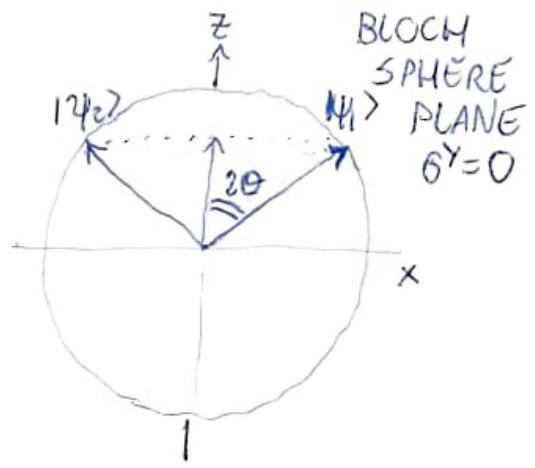
\includegraphics[width=0.5\textwidth, center]{2025_10_16_1bd50d0393172dac5e59g-02}\
$50 / 50$ HIXTURE $\quad \begin{cases}\left|\psi_{1}\right\rangle & p=\frac{1}{2} \\ \left|\psi_{2}\right\rangle & p=\frac{1}{2}\end{cases}$

$$
\begin{aligned}
\rho_{0}=\frac{1}{2}\left|\psi_{1} \times \psi_{1}\right|+\frac{1}{2}\left|\psi_{2} \times \psi_{2}\right| & =\frac{1}{2}\left(\begin{array}{cc}
\cos ^{2} \theta & \cos \sin \\
\cos \sin & s^{2}
\end{array}\right)+\frac{1}{2}\left(\begin{array}{cc}\c^{2} & -c s \\ -c s & s^{2}\end{array}\right) \\
\rho & =\left(\begin{array}{cc}\cos ^{2} \theta & 0 \\ 0 & \sin ^{2} \theta\end{array}\right) \quad \operatorname{Tr}[\rho]=1 \\
\rho & \geqslant 0
\end{aligned}
$$

$\rho$ - is $\left.\begin{array}{l}\text { ALSO MIXYRE OF } \\ |0\rangle \text { ANA } H\rangle\end{array}\right\} \quad \left\{\begin{array}{ll}|0\rangle & p=\cos ^{2} \theta \\ |1\rangle & p=\sin ^{2} \theta\end{array} \quad \rho=\cos ^{2} \theta|0 \times 0|+\sin ^{2} \theta|1 \times 1|\right.$

$$
\left\langle\sigma^{z}\right\rangle=\cos 2 \theta \quad\left\langle\sigma^{x}\right\rangle=\left\langle\sigma^{y}\right\rangle=0 \quad \sqrt{ } \text { CHECKS OUT }
$$

$\operatorname{Tr}\left[\rho^{2}\right]=\frac{1}{2}\left(1+\cos ^{2} 2 \theta\right) \xrightarrow{\longrightarrow}\left\{\begin{array}{l}2 \theta=0 \\ 2 \theta=\pi\end{array} \quad\right.\text { EXERCISE}
\\
|\psi(\varphi)\rangle=\binom{\cos \theta}{e^{i \varphi} \sin \theta}
\\
COMPETE UNCERTAINTY OVER $\varphi$

$$
d p(\varphi)=\frac{1}{2 \pi} d \varphi
$$

$\rho=\int|\psi(\varphi)\rangle\langle\psi(\varphi)| d p(\varphi)=\int_{0}^{2 \pi}\left(\begin{array}{cc}\cos ^{2} \theta & e^{-i \varphi} \sin \theta \cos \theta \\ \text { c.c. } & \sin ^{2} \theta\end{array}\right) \frac{d \varphi}{2 \pi}=\left(\begin{array}{cc}\cos ^{2} \theta & 0 \\ 0 & \sin ^{2} \theta\end{array}\right)\
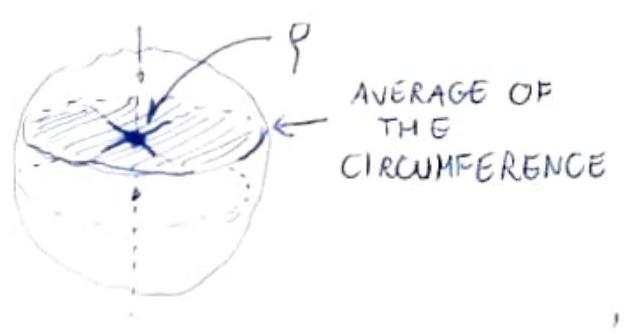
\includegraphics[width=0.5\textwidth, center]{2025_10_16_1bd50d0393172dac5e59g-03}\
closed system dynamics for sensity matrices
$\rho=\sum_{1} p_{\alpha}\left|\psi_{\alpha} \times \psi_{\alpha}\right|$ NO INTERFERENCE $\Rightarrow$ EVERY MEMBER EVOLVES BY ITSELF PROBABILITIES ARE STATIC $\dot{p}_{2}=0$

$$
\begin{array}{r}
\dot{\rho}=\sum^{\prime} p_{\alpha}\left|\dot{\psi}_{\alpha}\right\rangle\left\langle\psi_{\alpha}\right|+\sum p_{\alpha}\left|\psi_{\alpha}\right\rangle\left\langle\dot{\psi}_{\alpha}\right|=\sum p_{\alpha}\left(-\frac{i}{\hbar} H|\psi \times \psi|+\frac{i}{\hbar}|\psi \times \psi| H\right) \\
=\sum p_{\alpha} \frac{i}{\hbar}\left[i \psi_{\alpha} \times \psi_{\alpha} \mid, H\right]=\left[\sum p_{\alpha}\left|\psi_{\alpha} \times \psi_{\alpha}\right|, H\right] \frac{i}{\hbar}=+\frac{i}{\hbar}[\rho, H] \\
\dot{\rho}=\frac{i}{\hbar}[\rho, H] \quad \begin{array}{l}\text { SCHOÖSINGER EQ, } \\ \text { FOR SENSITY MATRICES } \\ \text { (SCHR PICTURE) }\end{array}\left(\begin{array}{c}\text { SIMICAR TO HEISENBERG } \\ \text { PICURE BUT WITH A } \\ \text { MINUS }\end{array}\right)
\end{array}
$$

GIBBS/BOLTZMANN
ENSEMBLE
$\rho=\frac{\exp \left(-\frac{H}{K_{B} T}\right)}{T_{r}\left[\exp \left(-\frac{H}{K_{B} T}\right)\right]}$
$\hat{L}$
GUANTUH SYSTEH IN CONTACY WITH FIXEST RESERVOIR EQUILIBRATES HERE
(1.) STATIONARY $\leftrightarrow$ EQUILIBRIUM
(2.) MAXIHISES $S$ AT FIXED INTERNAL ENERGY Tr [Hg] -OR-
(3.) HINIMIZES THE FREE ENERGY $F=\operatorname{Tr}[\mathrm{Hp}]-T S(\rho)$ at fixed $T$ TEMPERAYURE

FUT HOW TO GET THERE?

DIPARTTE SYSTEM $A$ B

$$
\left|\psi_{A B}\right\rangle=\sum_{a b} C_{a b}\left|\psi_{a}\right\rangle_{A} \underset{\uparrow}{\otimes}\left|\phi_{b}\right\rangle_{B}
$$

tensur product structure
an cbservabe Acting oncy on $A$

$$
\begin{aligned}
C_{A B}=\theta_{A} \otimes \mathbb{1}_{B} \quad\langle\theta\rangle & =\operatorname{Tr}\left[\left(\theta_{A} \otimes \mathbb{1}_{B}\right) \rho_{A B}\right]=\\
& =\sum_{a b}\left\langle\left.a\right|_{A}\left\langle\left.b\right|_{B}\left(\theta_{A} \otimes \frac{1}{B}\right) \rho_{A B} \right\rvert\, a\right\rangle_{A} \right\rvert\, b\right\rangle_{B} \\
& =\sum_{a b}\langle a| \theta_{A}\left\langle\left.b\right|_{B} \rho_{A B} \mid b\right\rangle_{B}|a\rangle_{A}=\\
& =\sum_{a}\langle a| \theta_{A} \rho_{A}|a\rangle=\operatorname{Tr}\left[\theta_{A} \rho_{A}\right]
\end{aligned}
$$

WHERE

$$
\rho_{A}=\Delta \sum_{b}^{1}\left\langle\left.b\right|_{B} \rho_{A B} \mid b\right\rangle_{B}=T_{B}\left[\rho_{A B}\right] \quad \text { TRACE (over B) }
$$

\begin{figure}[h]
\begin{center}
  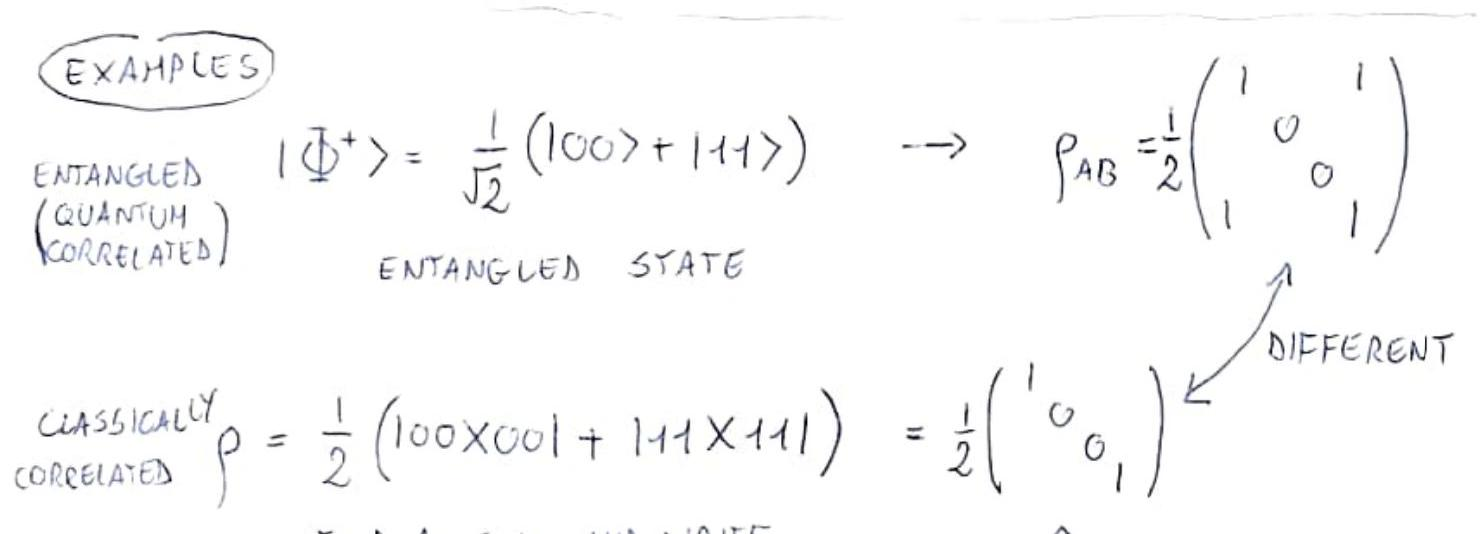
\includegraphics[width=\textwidth]{2025_10_16_1bd50d0393172dac5e59g-04}
\captionsetup{labelformat=empty}
\caption{介\\
NOT ENTANGED}
\end{center}
\end{figure}

$$
\rho_{A}=\frac{1}{2}\left(\begin{array}{ll}
1 & 0 \\ 0 & 1
\end{array}\right)=\frac{1}{2}
$$

completecy mixed

$$
\rho_{A}=\frac{11}{2} \text { SAME }
$$

FLIP A COIN AND WRITE the result twice
UNCCRRELAYED

$$
\rho=\frac{11}{2} A \otimes \frac{11}{2} B=\frac{1}{4}\left(\begin{array}{l}
1 \\ 1 \\ 1
\end{array}\right) \quad \rho_{A}=\frac{11}{2} \underset{\text { SAME }}{\text { CTME }}
$$

THE PARTIAL TRACE
HIDES/DELETES/AVERAGES OVER
CORRELATIONS (BETWEN A AND B)
QUAMTUM OR CLASSICAL

\section*{The Master Equation}
\begin{center}
\begin{tabular}{lll}
SYSTEM $\leftarrow$ & BATH & \begin{tabular}{l}
IN GENERAL, TO DESCRIBE THE SYNAMICS, \\
YOU NEES TO TRACK THE (QUANTUM) EVOLUTION \\
\end{tabular} \\
QUANTUM & \begin{tabular}{l}
QUANTUM \\
AND/OR \\
CLASSICAL \\
\end{tabular} & \begin{tabular}{l}
OF BOTH SYSTEM + BATH TOGETHER \\
TWHEN CAN WE SESCRIBE THE SYSTEM ALONE \\
\end{tabular} \\
 &  & AND DESCRIBE ITS EVOWTION ? \\
\end{tabular}
\end{center}

Born-Markov DYNAMICS
! WHEN... THE BATH LOSES IMMEDIATELY MEMORY OF THE SYSTEM (FOR SORE IT WORKS)

\begin{figure}[h]
\begin{center}
  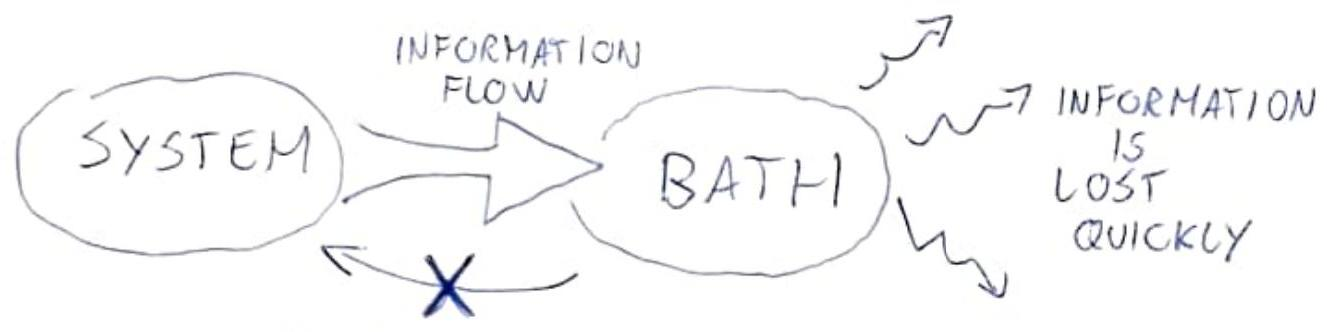
\includegraphics[width=\textwidth]{2025_10_16_1bd50d0393172dac5e59g-05}
\captionsetup{labelformat=empty}
\caption{INFOCMATION NEVER GOES BACK}
\end{center}
\end{figure}

\section*{Physical REQUIREMENT}
the bath must be fast and large
(1)

FAST

$$
\begin{aligned}
& H_{\text {TOT }}=H_{\text {SYS }}+H_{\text {BATH }}+H_{\text {WT }} \text { thescale } \\
& \text { SEPARATION } \\
& \tau_{B} \ll \tau_{b} \ll \tau_{\text {INT }} \\
& \text { REQUIRED } \\
& \text { FOR BORN-HARKOV } \\
& \text { APPROX } \\
& \begin{array}{l}\text { REQUIREA FOR } \\ \text { QUANUM } \\\text { DYNAMICS }\end{array} \\
& \text { the bath must have space } \\
& \text { to "STORE AND FORGET" INFO } \\
& \text { about the SYSTEM } \\
\end{aligned}
$$

$H=H_{S Y S}+H_{\text {BATH }}+H_{\text {INT }} \quad\binom{H_{B}=\mathbb{1}_{S} \otimes H_{B}}{H_{S}=H_{S} \otimes \mathbb{1}_{B}}$
\Step. 1 change reference frame - interaction pictore
$\left[U, H_{3} \otimes \Perp\right]=0<\left[U, 1 \otimes H_{3}\right]$

$$
\begin{aligned}
&\left.\begin{array}{l}\text { hamiltonian } \\ \text { of the new } \\ \text { frame }\end{array}\right\}
\end{aligned}
$$

COMPARE WITH THE
FORHAL IERIVATION FROM ADSITIVITY

$$
\left(H_{IW T}=\sum_{\alpha}^{1} S_{\alpha} B_{\alpha}\right)
$$

$$
\dot{\rho}^{\prime}(t)=+\frac{i}{\hbar}\left[\rho^{\prime}(t), H_{\text {INT }}(t)\right] \quad \downarrow \text { SIMPLE } \int_{0}^{t} d t
$$

(STEP.2) Integrate and plug-in

$$
\begin{aligned}
& \rho^{\prime}(t)=\rho^{\prime}(0)=\frac{i}{\hbar} \int_{0}^{t}\left[\rho^{\prime}(t), \tilde{H}_{M N}(t)\right] d t \quad\left(\begin{array}{c}\text { PLUE BACK INSIDE } \\ \text { THE EQUATION } \\ \text { AND GET... } \\ \rho^{\prime}(t)=\rho^{\prime}(0)+\frac{i}{\hbar} \int_{0}^{t}\left[\rho^{\prime}(t), \tilde{H}_{I N T}(t)\right] d t\end{array}\right. \\
& \dot{\rho}^{\prime}(t)=\underbrace{\frac{i}{\hbar}\left[\rho^{\prime}(0), \tilde{H}_{I N T}(t)\right]}_{\text { PIECE } \Delta}-\underbrace{\frac{1}{\hbar^{2}} \int_{0}^{t}\left[\left[\rho^{\prime}\left(t^{\prime}\right), \tilde{H}_{I N T}\left(t^{\prime}\right)\right], \tilde{H}_{I N T}(t)\right] d t^{\prime}}_{\text { PIECE } \square}
\end{aligned}
$$

BORN APPROXIMATION:

THE STATE OF THE BATH IS UNALTERES
$\rho(t)=\rho_{S}(t) \otimes \rho_{B}(0) \underset{\text { FRAME }}{\stackrel{\text { Interation }}{\text { TVAL }}} \rho^{\prime}(t)=\rho_{S}^{\prime}(t) \otimes \rho_{B}(0) \quad\binom{\left.H_{B}+H_{S}\right]}{\rho_{B}^{\prime}=\rho_{B}}$
$\operatorname{Tr}_{B}[$ PIECE $\Delta]=\frac{i}{\hbar} \operatorname{Tr}_{B}\left(\left[\rho_{S}^{\prime}(0) \otimes \rho_{B}(0), \check{H}_{\text {INY }}(t)\right]\right)=$
$=\frac{i}{\hbar} \sum_{\alpha}\left(\left[\rho_{s}^{\prime}(0), \tilde{S}_{\alpha}(t)\right] \operatorname{Tr}\left(\rho_{\beta}(0) \tilde{B}_{\alpha}(t)\right)\right)=\frac{i}{\hbar} \sum\left\langle\tilde{B}_{\alpha}\right\rangle\left[\rho_{s}^{\prime}(0), \tilde{S}_{\alpha}(t)\right]$
REDEFINE THE MODEL
$H_{s} \rightarrow H_{s}+\sum S_{\alpha}\left\langle B_{\alpha}\right\rangle$
$H_{I N T} \rightarrow \sum_{1} S_{\alpha}\left(B_{\alpha}-\left\langle B_{\alpha}\right\rangle\right)$
The second piece
The second piece
$\dot{\rho}_{S}^{\prime}(t)=+\frac{1}{\hbar^{2}} \int_{0}^{t} T_{B}\left(\left[\left[\tilde{H}_{\text {INT }}\left(t^{\prime}\right), \rho_{S}^{\prime}\left(t^{\prime}\right) \otimes \rho_{B}(0)\right], \tilde{H}_{\text {INT }}(t)\right]\right) d t^{\prime}$ NAKAJIMA-ZOWANZIG EQUATION

AFTER THIS RE-SEFINITION THE NEW $\left\langle B_{\alpha}\right\rangle=0$

$$
\operatorname{Tr}_{B}(P \mid E C E \Delta)=0 .
$$

$$
H_{I N T}=\sum_{\alpha} S_{\alpha}^{e} B_{\alpha}=\sum S_{\beta}^{+} \otimes B_{\beta}^{+}$
$$
\dot{\rho}_{S}^{\prime}(t)=\frac{1}{\hbar^{2}} \int_{0}^{t} \tilde{S}_{\alpha}\left(t^{\prime}\right) \rho_{s}^{\prime}\left(t^{\prime}\right) \tilde{S}_{\beta}^{\dagger}(t) \underbrace{\operatorname{Tr}\left[\rho_{\beta}(0) \tilde{B}_{\alpha}\left(t^{\prime}\right) \tilde{B}_{\beta}^{+}(t)\right]}_{\operatorname{Tr}\left[\rho(0) \tilde{B}^{\prime}(0) \tilde{B}^{+}(t-\theta)\right]}+\left(\begin{array}{c}\text {THER } \\ \text {THEREENIS } \\ \text { COMPONENT }\end{array}\right)
$$

PUTTING PIECES BACK
$\dot{\rho}_{S}^{\prime}(t)=+\frac{1}{\hbar^{2}} \sum_{\alpha \beta} \int_{0}^{t}\left\{\mathcal{G}_{\alpha \beta}\left(t-t^{\prime}\right)\left(\tilde{S}_{\alpha}\left(t^{\prime}\right)\right. \left.+C_{\beta \alpha}\left(t^{\prime}-t\right)\left(\breve{S}_{\beta}^{+}(t) \rho_{5}^{\prime}\left(t^{\prime}\right) \breve{S}_{\alpha}\left(t^{\prime}\right)-\rho_{5}^{\prime}\left(t^{\prime}\right) \widehat{S}_{\alpha}\left(t^{\prime}\right) \tilde{S}_{\beta}^{+}(t)\right)\right)\} d t$
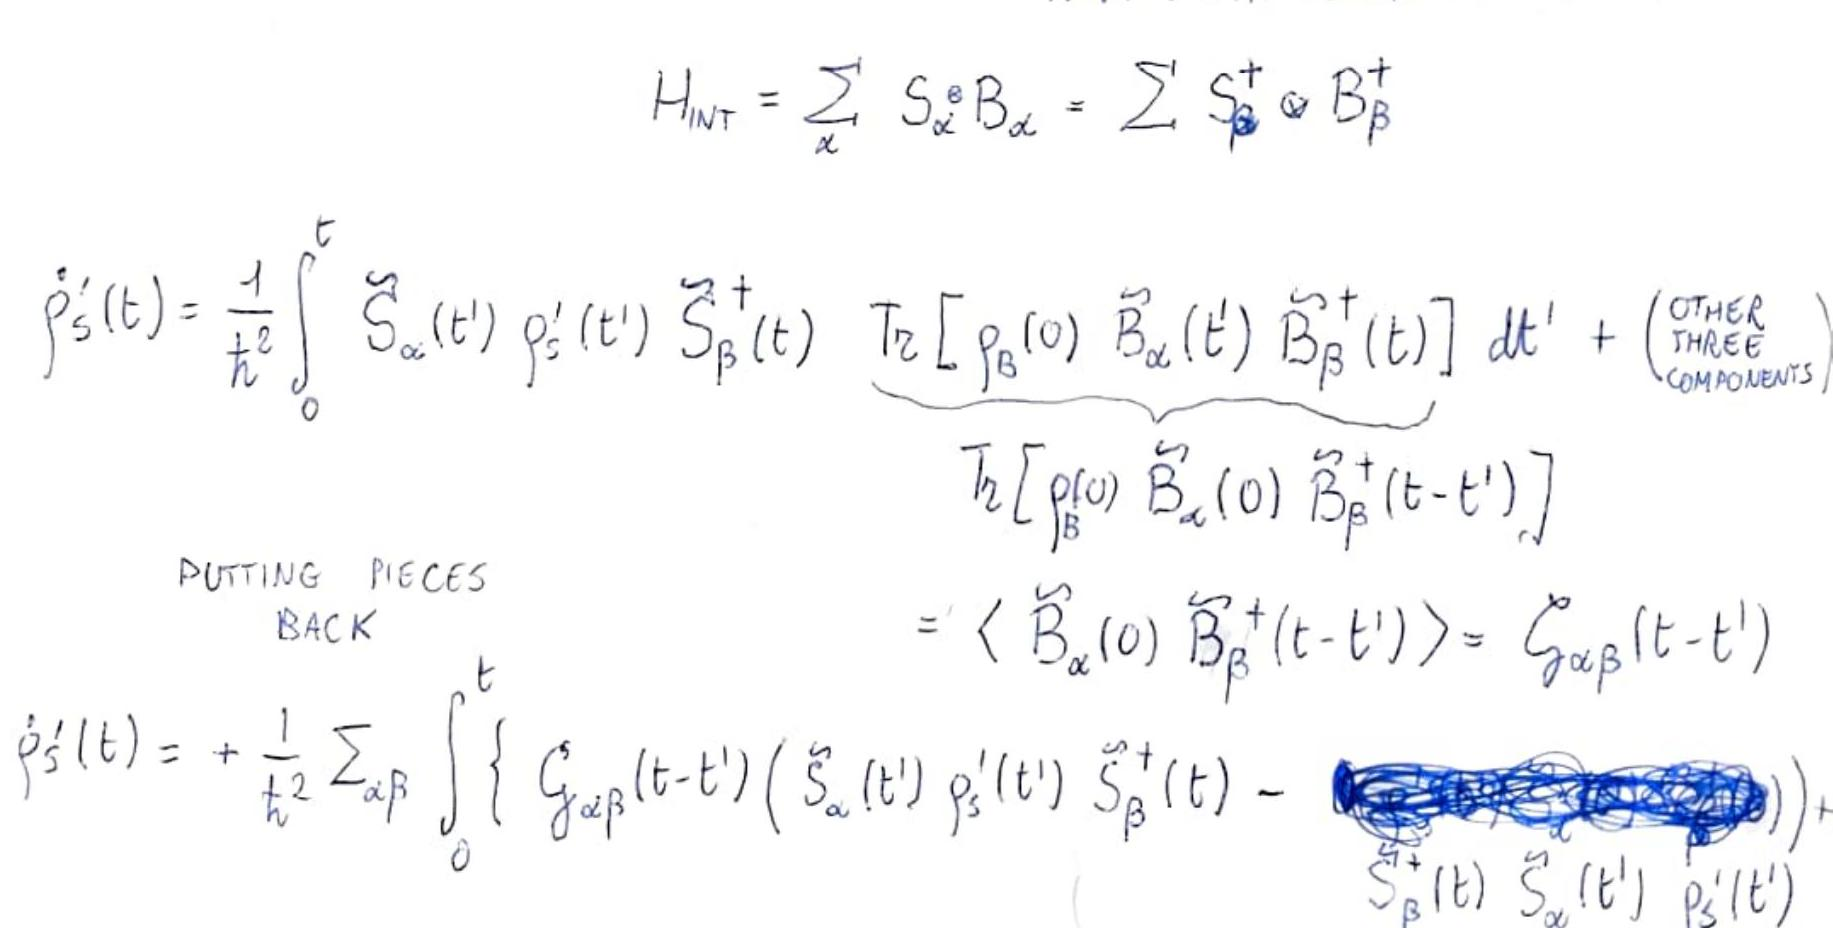
\includegraphics[width=0.5\textwidth]{2025_10_16_1bd50d0393172dac5e59g-07} ${ }_{\beta}^{+}(t) \tilde{S}_{\alpha}\left(t^{\prime}\right) \rho_{\beta}^{\prime}\left(t^{\prime}\right)$

\section*{MARKOV APPROXIMATION}
the correcations of the bath secay super fast

$$
\begin{array}{r}
\oint_{\alpha \beta}(t) \propto \zeta_{\alpha \beta}(0) \delta(t) \quad \text { 《 FOR SANITY, LET US } \\
\dot{\rho}_{S}^{\prime}(t)=\sum_{\alpha \beta} \zeta_{\alpha \beta}\left(\tilde{S}_{\alpha} \rho_{S}^{\prime} \tilde{S}_{\beta}^{+}-\tilde{S}_{\beta}^{+} \tilde{S}_{\alpha} \rho_{S}^{\prime}\right)_{t}+\zeta_{\beta \alpha}\left(\tilde{S}_{\beta}^{+} \rho_{S}^{\prime} \tilde{S}_{\alpha}-\rho_{S}^{\prime} \tilde{S}_{\alpha} \tilde{S}_{\beta}^{+}\right)
\end{array}
$$

BACK TO THE LAB FRAME $\rho_{5}(t)=e^{-i t H_{5}} \rho_{5} e^{+i t H_{5}}$

$$
\begin{aligned}
&\begin{array}{c}\dot{\rho}_{S}(t)=+i\left[\rho_{S}^{(t)}, H_{S}\right]+\sum_{\alpha \beta} G_{\alpha \beta}\left(S_{\alpha} \rho_{3}(t) S_{\beta}^{+}-S_{\beta}^{+} S_{\alpha} \rho_{s}(t)\right)+\underbrace{}_{\sum_{\alpha \beta}}\left(S_{\beta}^{+} \rho_{\beta}(t) S_{\alpha}-\rho_{S}(t) S_{2} S_{\beta}^{+},\\
\left\langle B_{\alpha} B_{\beta}^{r}\right\rangle
\end{aligned}
$$

$$ \text { USING } \begin{array}{ll} \text { II } & \text { EXTENS } \\ & \sum_{p}^{+} S_{p}^{+} B_{\beta}^{+} \end{array} \text { VECTOR OF } $$

$$ C_{\alpha \beta}\left(S_{\alpha} \rho S_{\beta}^{+}-\rho S_{\beta}^{+} S_{\alpha}\right) $$

$$
\rho_{s}=\frac{i}{\hbar}\left[\rho_{s}, H_{s}\right]+\sum_{\alpha \beta} C_{\alpha \beta}\left(2 S_{\alpha} \rho S_{\beta}^{+}-\left\{S_{\beta}^{+} S_{\alpha}, \rho\right\}\right)
$$

$$
\begin{aligned}
& G_{\alpha \beta}=\operatorname{Tr}\left[\rho_{\beta} B_{\alpha} B_{\beta}^{+}\right] \rightarrow G_{\alpha \beta} \quad \begin{array}{c}\text { IS POSITIVE } \\ \text { SEMISEINITE }\end{array} \rightarrow \begin{array}{c}\text { CAN BE } \\ \text { DIAGONALIZES } \\ u_{\alpha Y}^{+} \gamma_{j}^{N} u_{j \beta} \\ \text { REDEFINE } L_{j}=\sum_{\alpha} u_{j, \alpha} S_{\alpha} \sqrt{2}\end{array}
\end{aligned}
$$

DIMENSIONLESS LINDBLADIANS

$$
\begin{array}{r}
\dot{\rho}_{S}=\frac{i}{\hbar}\left[\rho_{1} H_{3}\right]+\sum_{J} \int_{\prod_{S}}\left(L_{J}^{\downarrow} \rho L_{J}^{+}-\frac{1}{2}\left\{L_{J}^{+} L_{J}, \rho\right\}\right) \\
\geqslant 0 \text { DIMENSION OF } t^{-1} \quad \rho=\mathcal{L}(\rho)
\end{array}
$$

lindscas master equation

NOTICE $\frac{d}{d t} T r[\rho]=0 \leftarrow$ no coss of tOTAL PROBABICITY\[0pt]example 1 [harkovian dynamics] Decay

2-hevel system

\begin{itemize}
  \item ${ }^{|e\rangle}$
\end{itemize}

$$
H_{s}=\hbar \omega|e \times e| $$

$\frac{\sum_{2}}{|y|}$\
ONE

$$
\rho_{0}=\left(\begin{array}{ll}a_{0} & b_{0} \\ b_{0}^{*} & c_{0}\end{array}\right)
$$

WHERE

$$
c_{0}=1-a_{0}
$$

$\underbrace{\left|b_{0}\right|^{2} \leqslant a_{0} c_{0}}_{\substack{\text { POSITIVITY } \ \text { CONDITION }}}$

$$
\rho(t)=\left(\begin{array}{ll}a(t) & b(t) \\ b^{*}(t) & c(t)\end{array}\right)
$$

$\dot{\rho}(t)=-\frac{i}{\hbar} H_{\downarrow} \rho+\frac{i}{\hbar} \rho H+\gamma L \rho L^{+}-\frac{1}{2} \gamma L^{+} L \rho-\frac{\gamma}{2} \rho \underbrace{\rho L^{+} L}_{\downarrow}$\
$H=\hbar \omega\left(\begin{array}{ll}0 & 0 \\ 0 & 1\end{array}\right) \quad\left(\begin{array}{ll}0 & 1 \\ 0 & 0
\end{array}\right) \quad\left(\begin{array}{ll}0 & 0 \\ 1 & 0
\end{array}\right) \quad\left(\begin{array}{ll}0 & 0 \\ 0 & 1
\end{array}\right)$
$\left(\begin{array}{cc}\dot{a} & \dot{b} \\ \dot{b} & \dot{c}\end{array}\right)=i \omega\left(\left(\begin{array}{ll}0 & b \\ 0 & c
\end{array}\right)-\left(\begin{array}{cc}0 & 0 \\ b^{*} & c
\end{array}\right)\right)+\gamma\left(\left(\begin{array}{ll}c & 0 \\ 0 & 0
\end{array}\right)-\frac{1}{2}\left(\begin{array}{ll}0 & 0 \\ b^{*} & c
\end{array}\right)-\frac{1}{2}\left(\begin{array}{ll}0 & b \\ 0 & c
\end{array}\right)\right)$
DIFFERENTIAC EQCATIONS FOR $b$ ANS $c \rightarrow$ EASY

$$
\begin{cases}\begin{array}{l}\dot{b}=\left(i \omega-\frac{\gamma}{2}\right) b(t) \\ \dot{c}=-\gamma c(t)\end{array} \Rightarrow & b(t)=b_{0} e^{\left(i \omega-\frac{\gamma}{2}\right) t} \ll \text { SPIRAL } \\ a=(1-c) & c(t)=c_{0} e^{-\gamma t} \geqslant 0 \\ \rho(t)=\left(\begin{array}{cc}\n1-c_{0} e^{-\gamma t} & e^{\left(i \omega-\frac{\gamma}{2}\right) t} b_{0} \\ e^{\left(-i \omega-\frac{\gamma}{2}\right) t} b_{0}^{*} & c_{0} e^{-\gamma t}\end{array}\right) \\ \downarrow t \rightarrow \infty \text { STEADY STATE } \\ \rho(t=\infty)=\left(\begin{array}{ll}1 & 0 \\ 0 & 0
\end{array}\right)=|g \times g|\end{cases}
$$

\section*{Example 2 Dephasing}
$$
L=L^{+}=L^{+} L=\left(\begin{array}{ll}0 & 0 \\ 0 & 1
\end{array}\right)=H \frac{1}{\hbar \omega}
$$

$$
\begin{aligned}
& H=\hbar \omega(e \times e) \\
& L=|e \times e| \text { ANE } \gamma\left\{\begin{array}{l}\text { PROBABILIST } \\ \text { FUPP }\end{array}\right.
\end{aligned}
$$
$\left(\begin{array}{cc}\dot{a} & \dot{b} \\ b^{*} & \dot{c}\end{array}\right)=i \omega\left(\begin{array}{cc}0 & b \\ b^{*} & 0
\end{array}\right)+\gamma\left(\left(\begin{array}{ll}0 & 0 \\ 0 & c
\end{array}\right)-\frac{1}{2}\left(\begin{array}{ll}0 & b \\ 0 & c
\end{array}\right)-\frac{1}{2}\left(\begin{array}{ll}0 & 0 \\ b^{*} & c
\end{array}\right)\right) c(t)=c_{0} \quad a(t)=1-c_{0} \quad b(t)=e^{\left(i \omega-\frac{\gamma}{2}\right) t} b_{0}$

$$
\begin{aligned}
& \left\langle\sigma^{2}\right\rangle(t)=a(t)-c(t)=1-2 c_{0} \text { constant } \\
& \left\langle\sigma^{*}\right\rangle(t)=\operatorname{tr}\left[\left(1^{\prime}\right)\left(\begin{array}{ll}\\
a & b \\ b^{*} c
\end{array}\right)\right]=b+b^{*}=e^{-\frac{\gamma}{2} t} \operatorname{Re}\left(e^{i \omega t} b_{0}\right)
\end{aligned}
$$

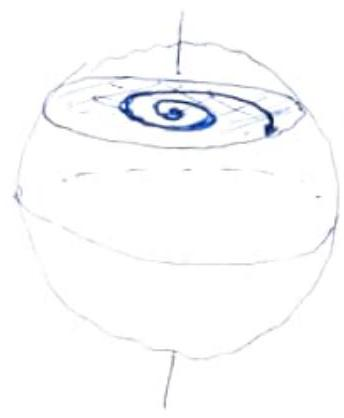
\includegraphics[width=0.5\textwidth, center]{2025_10_16_1bd50d0393172dac5e59g-10}\
$\\leftarrow$ Trasectory:

$$
\left(b_{0} R E A L\right)=e^{-\frac{\gamma}{2} t} \cos (\omega t) b_{0}
$$

IN-PLANE SPIRAL
steady syate(s)

$$
\rho(t=\infty)=\left(\begin{array}{cc}1-c_{0} & 0 \\ 0 & c_{0}\end{array}\right)
$$

NON-ONIQUE because of CONSERVES $\left\langle\sigma^{z}\right\rangle$

Dephasing 2.0
$p_{\substack{F_{1} x \\ D \\ \omega}}(t)=\left(\begin{array}{cc}1-c_{0} & b_{c} e^{+i \omega t} \\ b_{0}^{*} e^{-i \omega t} & c_{0}\end{array}\right)$
$\int_{\substack{\text { HEMSTICONNN } \\ \text { ENSEHRE }}}$

$$
\begin{array}{r}
=\left(\begin{array}{cc}1-c_{0} & b_{0} \int e^{i \omega t}\left(\frac{d \rho}{d \omega}\right) d \omega \\ c & c_{0}\end{array}\right) \\
\rho_{t>0}(t)=\left(\begin{array}{cc}1-c_{0} & e^{\left(i \omega_{0}-\gamma\right) t} \\ c . c & c_{0}\end{array}\right)
\end{array}
$$

no bath but cuasical

$$
H=\text { iexei } \hbar \omega
$$

probability density $\overbrace{\text {RANDOM }}^{\text {VARIABLE (STATIC) }}$

$$
\left\{\begin{array}{l}\int \frac{d p}{d \omega} \cdot d \omega=\int d p(\omega) \\ \frac{d p}{d \omega}=\frac{1}{\pi} \frac{\gamma}{\left(\omega-\omega_{0}\right)^{2}+\gamma^{2}} \\ \text {(AUCHY-CORGNZIZ SISTRP)}
\end{array}\right.
$$

BUT $\int_{-\infty}^{+\infty} \frac{d \omega}{\pi} \frac{\gamma e^{i \omega t}}{\left(\omega-\omega_{0}\right)^{2}+\gamma^{2}}=e^{i \omega_{0} t-\gamma|t|} \leftarrow \quad$ IDENTICAL TO PREVIOUS
EXERCISE. HARKOUAT DYNAMICS
ALSO MODELS NOISE (SOME FORHS)
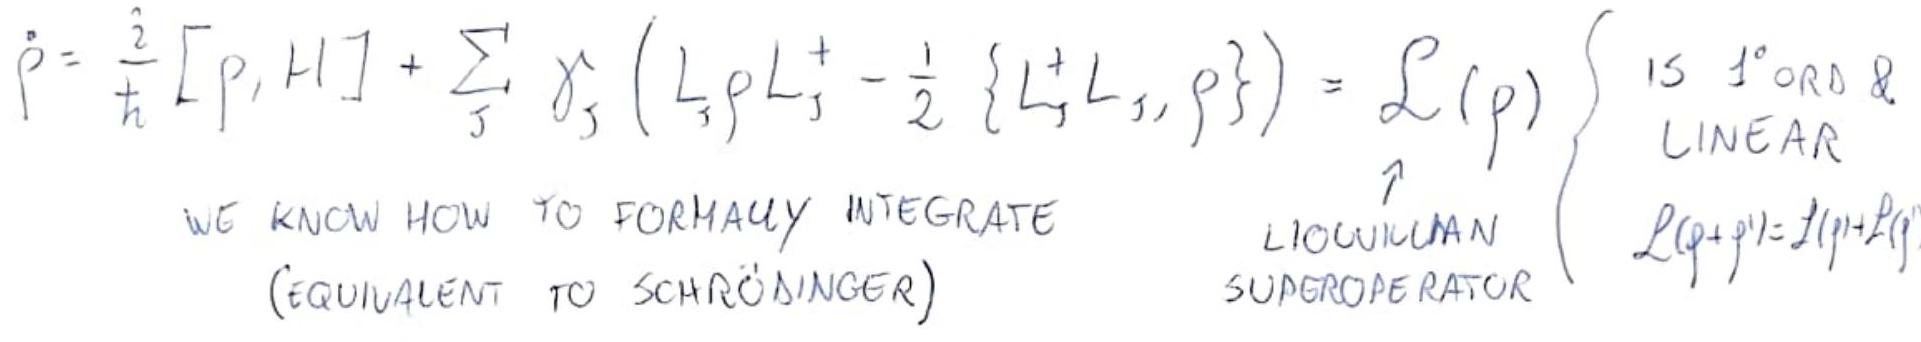
\includegraphics[width=0.5\textwidth, center]{2025_10_16_1bd50d0393172dac5e59g-11}\
TURN $\rho$ FROM MATRIX TO VECTOR $\hat{\rho} \rightarrow|\rho\rangle\rangle \quad \hat{\rho}$ SIMENSION $d_{H} \times d_{H}$
UKE THIS $|i\rangle
\langle J| \rightarrow|i J
angle\rangle$

$$
|p\rangle \text { SIMENSION } d_{H}^{2} \times 1
$$

$$
\stackrel{\text { SO THAT }}{\longrightarrow}\left(\begin{array}{ll}a & b \\ c & d\end{array}\right) \rightarrow\left(\begin{array}{l}a \\ b \\ c \\ d
\end{array}\right) \quad \begin{gathered}\text { SOMESTHES } \\ \text { KNOWN AS } \\ \text { CHOI TRANSFORY }
\end{gathered}
$$
PROPERTIES
HILBERT-SCHMIAT PRODUCY ON OPS
$T_{r}
[o_{p}]=
$\nA p B $\xrightarrow{C 401} A \otimes B_{\text {TRAN SDOSE }}^{t}|p
angle$

$$
\begin{aligned}
\operatorname{Tr}\left[A^{+}, B
ight] &=(A, B) \\
& =\langle\langle A \mid B\rangle\rangle
\end{aligned}
$$
IN CANONCAL BASIS

$$
\left.\left.=\langle\| 1| \sigma_{\theta} 1|\rho\rangle\right\rangle=\langle\langle 1| 1| \otimes \sigma^{*} |\rho\rangle\right\rangle=\left\langle\left\langle\theta^{(t)} \mid \rho\right\rangle\right
angle
$$
hataix ecemeny

$$
\rho_{i j}=\langle i| \rho|j\rangle=\langle\langle i j \mid \rho
angle\rangle
$$
The llouviulan as supermatrix $\hat{\hat{L}}$ (in choi teansform)
$\left.|
\dot{\rho}\rangle\right\rangle=\hat{\mathcal{L}}_{\hat{\rho}}^{\hat{\alpha}}|
ho
angle\rangle=\left(-\frac{i}{\hbar} H \otimes \mathbb{1}+\frac{i}{\hbar} \mathbb{1} \otimes H^{*}+\sum_{J} \chi_{J}\left(L_{J} \otimes L_{J}^{*}
ight.
ight.$

IF $\mathcal{L}$ に
time independent

$$
\left.\left.\left.\n-\frac{1}{2} L_{J}^{+} L_{J} \otimes \mathbb{1}-\frac{1}{2} \mathbb{1} \otimes L_{J}^{t} L_{J}^{*}\right)\right) d \rho\right\rangle\rangle
$$

HOWEVER $\hat{l}$ IS NOT HERMITIAN.
$|
ho(t)
angle\rangle=\exp ($ 总 $t)|
ho_{0}
angle\rangle$
IFE $\mathcal{L}$ CAN BE SIAGONACIZES $\quad \times D X^{-1}$

$$
\left.|
ho(t)
angle\right\rangle=x e^{D t} x^{-1}|
ho_{0}
angle\rangle
$$
(A) Exploding solutions are not physical, so $orall \\\lambda \in D, \operatorname{Re}(\\\lambda) \leqslant 0$ negative real part
(B) Steady state $|
\dot{p}
\rangle\rangle=0 《 \Leftrightarrow
\rangle 
\hat{\hat{\mathcal{L}}}|
ho
angle\rangle=0$ FOR THE LIOUVILIAN SPEC
ipst most be in the KERNEL of $\mathcal{L}$
! NOT ALL EIGENVECTORS ARE DENSITY MATRICES!
IN FACT

$$
\left.\left(\begin{array}{l}1 \\ 0 \\ 0 \\ 1
\end{array}\right)=|\mathbb{1}|>\right
angle
$$

$|
\dot{\rho}\rangle\rangle=\mathcal{L}|
ho
angle\rangle$ meserves the norm $\operatorname{Tr}[\rho]=\operatorname{Tr}
[j^{+} \rho]=\langle\langle
\mathbb{I} \mid \rho
angle
angle$
$\left.\left.\
\text { IHIS } \\ 	ext { THES } \\ \rightarrow \underline{\mathcal{L}|v
angle}=\lambda|v
angle\right\rangle \quad |v(t)
angle\rangle=e^{\lambda t}
|v_{0}
angle\rangle$ if $\operatorname{Re}(\\\lambda)<0$ EIGENVECTOR

$$
\operatorname{Tr}
[v_{0}]=\operatorname{Tr}[v(t)]=\sum_{<1}^{e^{\lambda t}} \operatorname{Tr}
[v_{0}]
$$

$\left\{\begin{array}{l}\text { ALL DECAYING } \\ \text { EIGEN-SUPERVECTORS } \\ \text { ARE TRACELESS }\end{array}\right.$
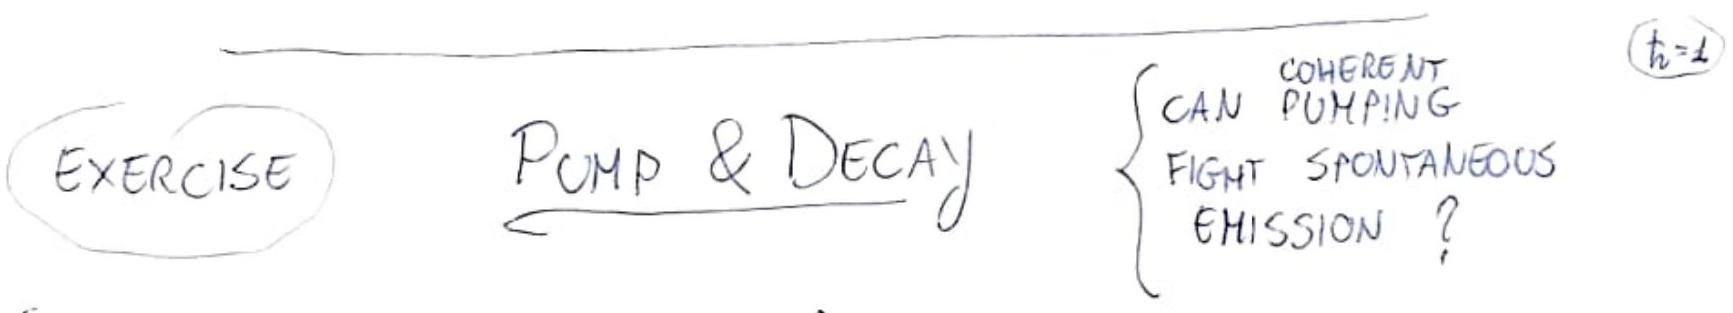
\includegraphics[width=0.5\textwidth, center]{2025_10_16_1bd50d0393172dac5e59g-12(1)}\
$\left\{\begin{array}{l}H=\Omega \sigma^{x}=\Omega(|g\rangle
\langle e|+|e
angle \\
L=|g\rangle
\langle e| \text { WIH RATE } \gamma
\end{array}\right.$

$$ e\rangle
\langle g|)
$$

$\sigma^{+}$

$$
H=\Omega\binom{1}{1} \quad L=\left(\begin{array}{ll}0 & 1 \\ 0 & 0
\end{array}\right) \quad L^{+} L=\left(\begin{array}{ll}0 & 0 \\ 0 & 1
\end{array}\right)
$$

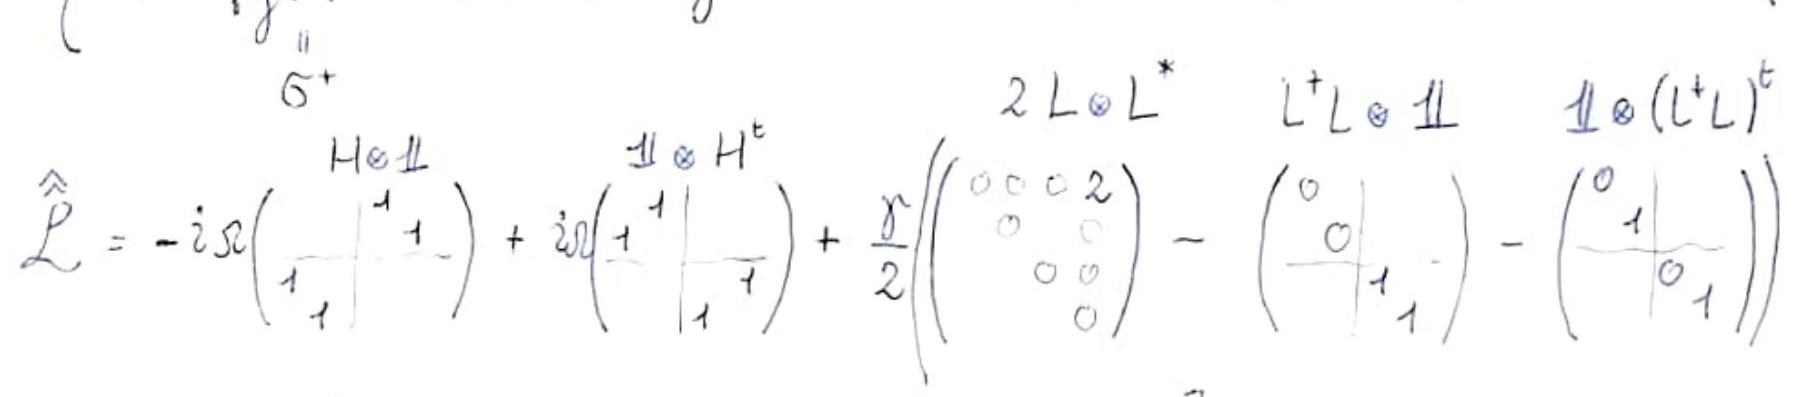
\includegraphics[width=0.5\textwidth, center]{2025_10_16_1bd50d0393172dac5e59g-12}\
$\hat{\mathcal{L}}=\Omega
\left[\left(\begin{array}{cccc}0 & i & -i & \\ i & 0 & & -i \\ -i & & 0 & i \\ & & -i & i \\ & & 0
\end{array}\right)+\frac{\gamma}{2 \Omega}\left(\begin{array}{lll}0 & & \\ & -1 & \\ & & -1 \\ & & \\ & & \\ & & \\ & & \end{array}\right)\right]$

% Lecture file created by Gemini
% Class: Quantum Information With Atoms and Photons
% Professor: Pietro Silvi
% Date: 2025-10-16
\lecture{4}{Alkali and dipole selection rules}{2025-10-16}

% --- Start writing here ---
\captionsetup{singlelinecheck=false}
Atoms of Group I From Hydrogen to Alkall\\
$\rightarrow$ THREE LEVELS OF DEPTM (PERTURBATION SPLIT)\\
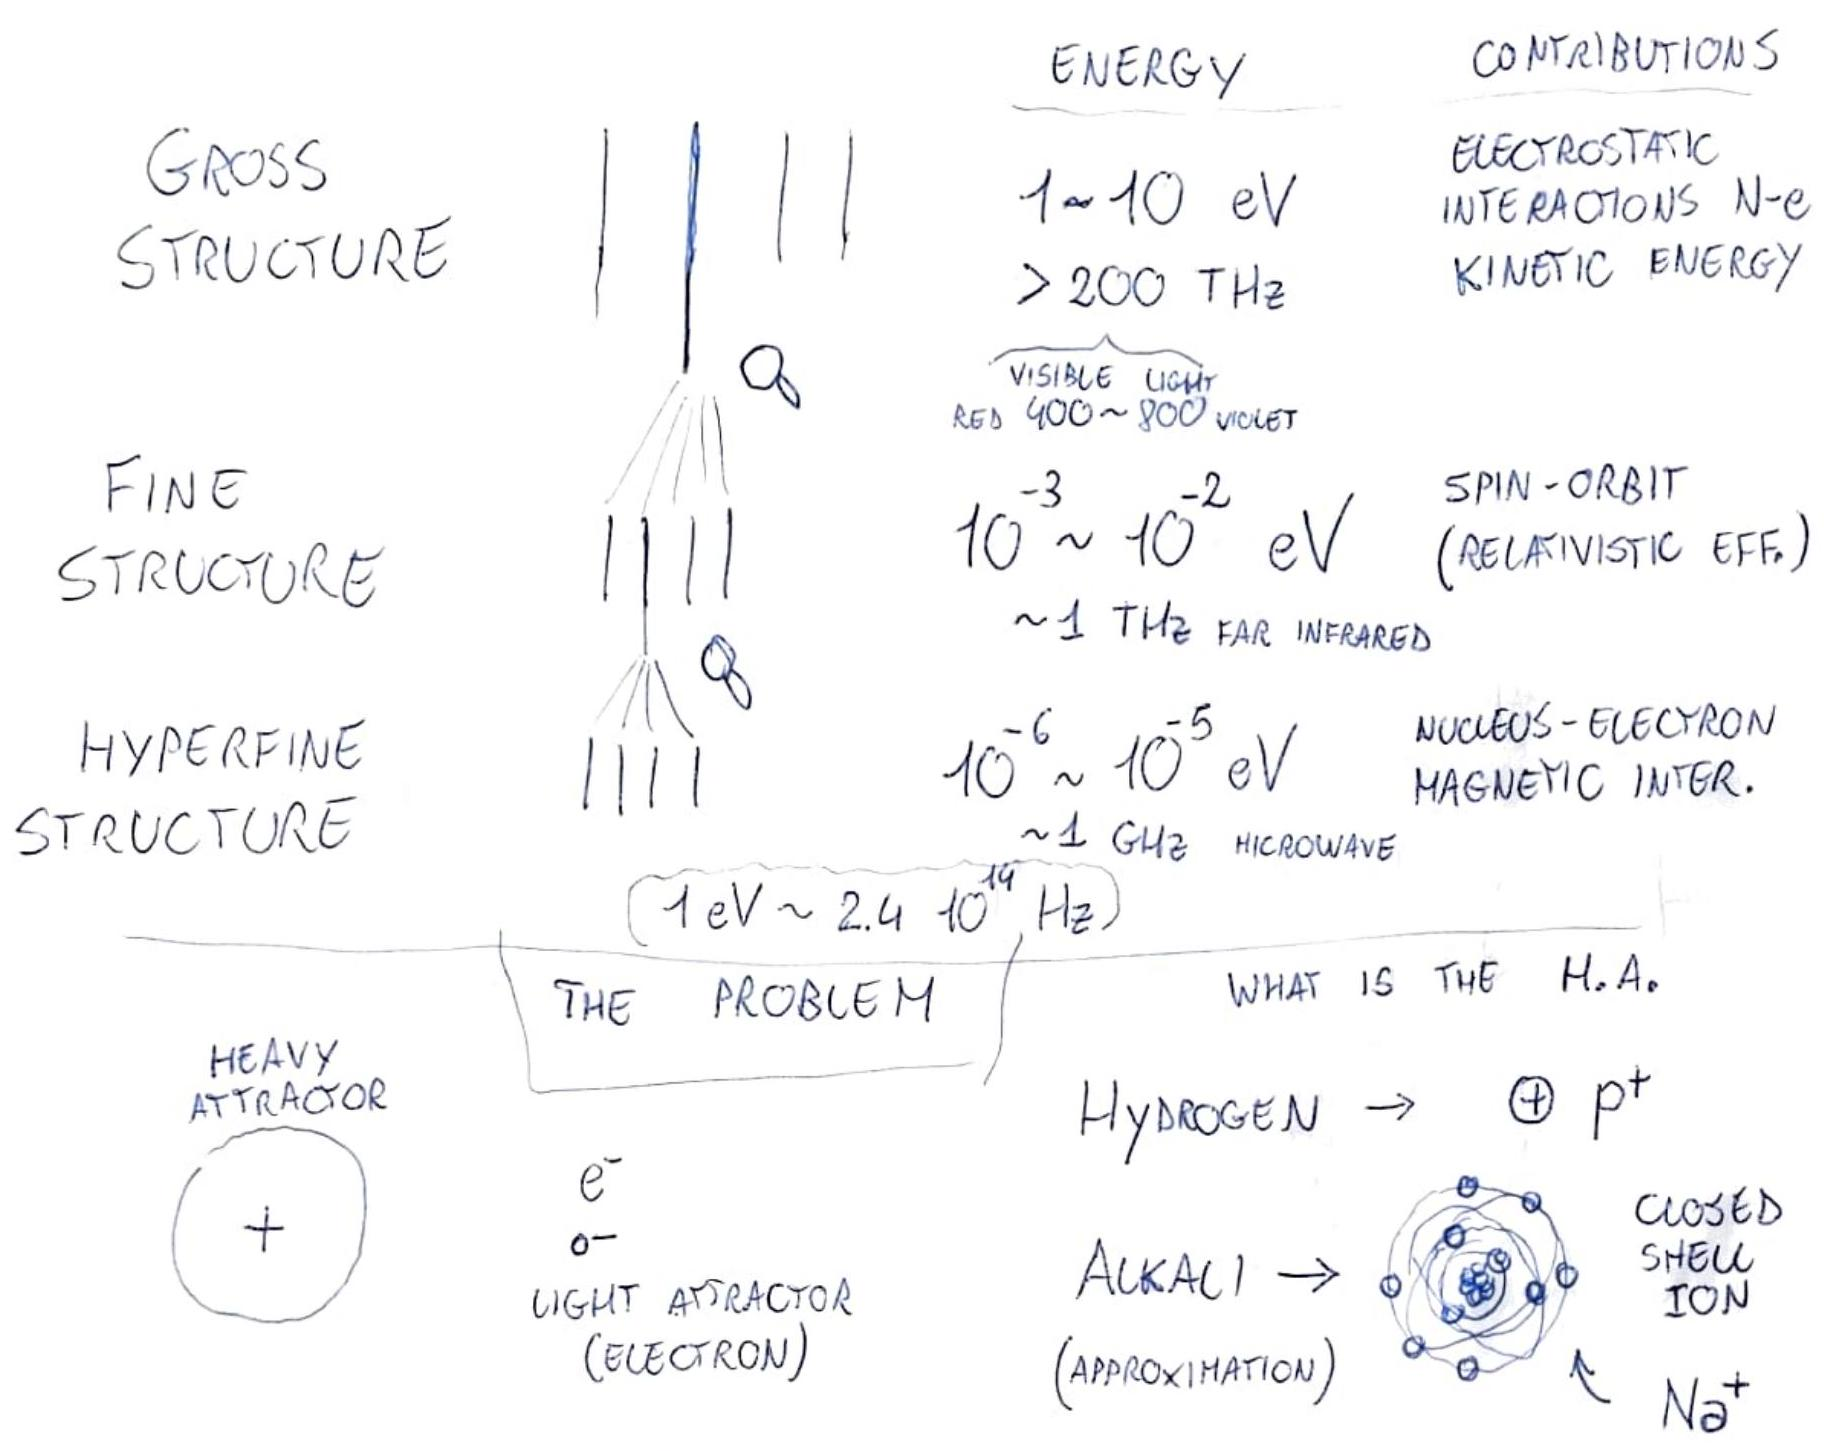
\includegraphics[max width=\textwidth, center]{2025_10_16_22329e0f50bdd2511b17g-01}

Effective 2-BODY Dynamics:

$$
H=\underbrace{\frac{\left|\vec{p}_{H}\right|^{2}}{2 m_{H}}}_{\substack{\text { HEAYY KINETIC } \\ \text { (NON RELATIVISTIC) }}}+\underbrace{\frac{\left|\vec{p}_{e}\right|^{2}}{2 m_{e}}}_{\substack{\text { ELECTRON KINETK } \\ \text { (SOMEHON STILU } \\ \text { NON RELATIVISTIC }}}+\overbrace{V\left(\left|\vec{r}_{H}-\vec{r}_{e}\right|\right)}
$$

Step 1 change of coorsinates

$$
\begin{gathered}
\text { CENTER-OF-MASS } \\
\text { COORDINATE } \\
\text { AND HOMENTUM }
\end{gathered}
$$

$$
\vec{R}=\frac{\vec{r}_{e} m_{e}+\vec{r}_{H} m_{H}}{m_{e}+m_{H}} \quad \vec{P}=\vec{P}_{e}+\vec{P}_{H}
$$

$$
\begin{aligned}
& \text { RELATIVE } \\
& \text { COORDINATE } \\
& \text { AND MOMENTUM }
\end{aligned}
$$

$$
\vec{r}=\vec{r}_{e}-\vec{r}_{H} \quad \vec{p}=\frac{\frac{\vec{p}_{e}}{m_{e}}-\frac{\vec{p}_{H}}{m_{H}}}{\frac{1}{m_{E}}+\frac{1}{m_{H}}}
$$

$$
\begin{gathered}
{\left[r_{e}, p_{e}\right]=i \hbar} \\
{\left[r_{H}, p_{H}\right]=i \hbar} \\
{\left[r_{e}, p_{H}\right]=\left[r_{H}, p_{e}\right]=0}
\end{gathered} \quad \backsim \quad\left[\begin{array}{l}
{[R, P]=[r, P]=i \hbar} \\
{[R, P]=[r, P]=0}
\end{array}\right.
$$

$$
m_{t}=m_{e}+m_{H} \approx m_{H}
$$

Where TOTAL HASS

$$
\begin{array}{r}
\frac{1}{m^{2}}=\frac{1}{m_{e}}+\frac{1}{m_{H}} \approx \frac{1}{m_{e}} \\
\text { RESUCES HASS }
\end{array}
$$

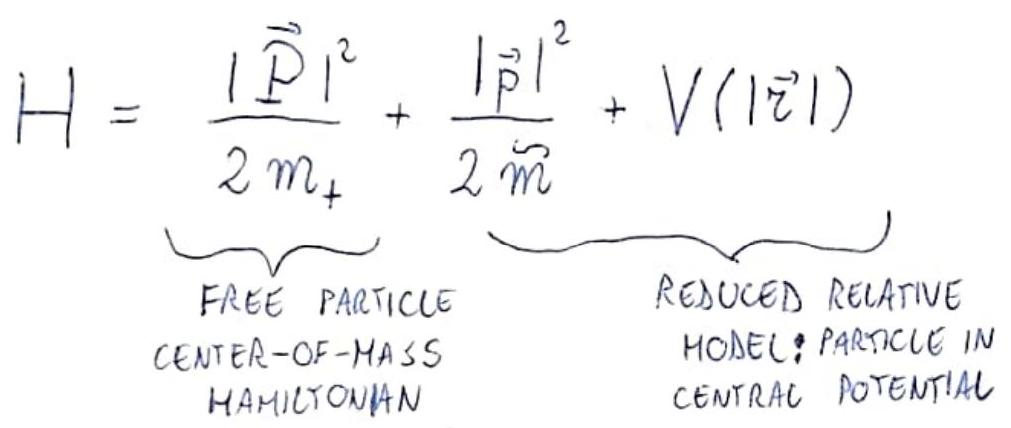
\includegraphics[max width=\textwidth]{2025_10_16_22329e0f50bdd2511b17g-02} $\binom{\text { but not helways }}{\text { refe! Recolu }} \longleftrightarrow$ we can ignore this part for now

$$
\begin{aligned}
& \frac{|\vec{p}|^{2}}{2 \vec{m}}=\left(\begin{array}{c}
\text { CARTESIAN } \\
\text { COORDINES } \\
x, y, z
\end{array}\right) \cdot \frac{-\hbar^{2}}{2 \vec{m}}\left(\frac{\partial^{2}}{\partial x^{2}}+\frac{\partial^{2}}{\partial y^{2}}+\frac{\partial^{2}}{\partial z^{2}}\right) \\
& \text { EASY TO } \\
& \text { REMEMBER } \\
& = \\
& -\frac{\hbar^{2}}{2 m} \nabla^{2}\left(\begin{array}{c}
\text { POLAR } \\
\text { CORDMATES } \\
r, \theta, \varphi
\end{array}\right)-\frac{\hbar^{2}}{2 m}\left(\frac{1}{r^{2}} \frac{\partial}{\partial r}\left(r^{2} \frac{\partial}{\partial r}\right)+\frac{1}{r^{2} \sin \theta} \frac{\partial}{\partial \theta}\left(\sin \theta \frac{\partial}{\partial \theta}\right)+\frac{1}{r^{2} \sin ^{2} \theta} \frac{\partial^{2}}{\partial \varphi^{2}}\right) \\
& =-\frac{\hbar^{2}}{2 m}\left(\frac{1}{r^{2}} \frac{\partial}{\partial r}\left(r^{2} \frac{\partial}{\partial r}\right)\right)+\frac{1}{2 m r^{2}} L^{2} \\
& \text { 正 } \\
& \text { angular momentum. } \\
& \text { We nees a refresher }
\end{aligned}
$$

\section*{Orbital angular Momentum}
of a canchical pairi coor $\vec{r}$ inate $+\underset{\vec{p}}{\text { homentum }}$(lhe resuces (ones in this case)\\
reads $\vec{L}=\underbrace{\vec{r} \times \vec{p}}_{\substack{\text { VECTCR CROSS } \\ \text { PROSUCT }}} \quad \begin{gathered}\text { CIASSICAL-OR-} \\ \text { QUANUMAMCS } \\ \text { HECHANICS }\end{gathered}$\\
COHMUTE THUS ALSO\\
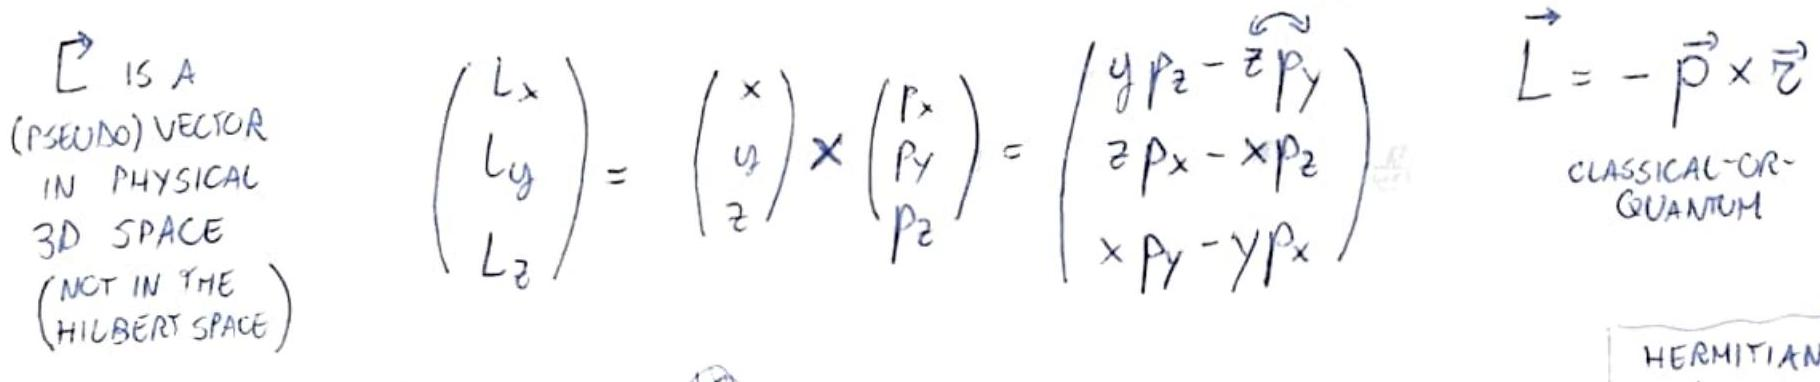
\includegraphics[max width=\textwidth, center]{2025_10_16_22329e0f50bdd2511b17g-03}

\section*{QUANTUM}
$\vec{r}$ and $\vec{P}$ are vectors $\quad L_{z}=-i \hbar\left(x \frac{\partial}{\partial y}-y \frac{\partial}{\partial x}\right)$ ete... OF OPERATORS,THLS\\
$\vec{L}$ as we U\\
$\vec{r}$ and $\vec{p}$ do not commute $D>L_{x}, L_{y}, L_{z}$ do not commute as well

$$
\begin{aligned}
& {\left[L_{x}, L_{y}\right]=-\hbar^{2}\left(\left(y \frac{\partial}{\partial z}-z \frac{\partial}{\partial y}\right)\left(z \frac{\partial}{\partial x}-x \frac{\partial}{\partial z}\right)-\left(z \frac{\partial}{\partial x}-x \frac{\partial}{\partial z}\right)\left(y \frac{\partial}{\partial z}-z \frac{\partial}{\partial y}\right)\right)} \\
& =-\hbar^{2}\left(y \frac{\partial}{\partial x}+y z \frac{\partial^{2}}{\partial z \partial x}-z^{2} \frac{\partial^{2}}{\partial x \partial y}-x y \frac{\partial^{2}}{\partial z^{2}}+x z \frac{\partial^{2}}{\partial y \partial z}\right)+ \\
& +\hbar^{2}\left(y z \frac{\partial^{2}}{\partial x \partial z}+x \frac{\partial}{\partial y}-x y \frac{\partial^{2}}{\partial z^{2}}-z^{2} \frac{\partial^{2}}{\partial x \partial y}+x z \frac{\partial^{2}}{\partial z \partial y}\right)= \\
& =\hbar^{2}\left(x \frac{\partial}{\partial y}-y \frac{\partial}{\partial x}\right)=i \hbar\left(x p_{y}-y p_{x}\right)=i \hbar L_{z} \text { AND BY EXTENGION } \\
& {\left[L_{i}, L_{j}\right]=i \hbar \underbrace{\varepsilon_{i jk}} L_{k}} \\
& \text { COMPUETECY ANTISYMMETRIC } \\
& \text { TENSOR } \\
& \text { TOTAL Angular } L^{2}=L_{x}^{2}+L_{y}^{2}+L_{z}^{2} \\
& \stackrel{\downarrow}{\text { commutes }}\left[L^{2}, L_{j}\right]=0 \quad \begin{array}{l}
\text { QUADRATIC } \\
\text { CASIMIR or. }
\end{array} \\
& \text { 《集 Closes lie Algebra } \\
& \text { OF HERMITIAN OPS. } \\
& \text { they generate continuous } \\
& \text { GROUPS (OF ROTATIONS) }
\end{aligned}
$$

EXAMPLE $\left[l^{2}, l_{z}\right]=\left[l_{x}^{2}, l_{z}\right]+\left[l_{y}^{2}, l_{z}\right]=$

$$
\begin{aligned}
& L_{x}^{2} L_{z}-L_{z} L_{x}^{2}+L_{y}^{2} L_{z}-L_{z} L_{y}^{2}= \\
& L_{x} L_{z} L_{x}+L_{x}\left[L_{x} L_{z}\right]-L_{x} L_{z} L_{x}-\left[L_{z} L_{x}\right] L_{x}+\ldots . .= \\
& \quad L_{x}\left(-i L_{y}\right)-\left(i L_{g}\right) L_{x}+L_{y}\left(+i L_{x}\right)-\left(-i L_{x}\right) L_{y}=0
\end{aligned}
$$

$\underset{\substack{\text { RAISING AND } \\ \text { COWERING }}}{\text { OPERATORS }}\left\{\begin{array}{l}L_{ \pm}=L_{x} \pm i L_{y} \leftarrow \text { NOT HERMITIAN }\left(L_{+}\right)^{+}=L_{x}^{+}+(i)^{*} L_{y}^{+}=L_{-} \\ {\left[L_{+}, L_{-}\right]=i\left[L_{y}, L_{x}\right]-i\left[L_{x}, L_{y}\right]=2 \hbar L_{z}} \\ {[1,1]}\end{array}\right.$

$$
\begin{aligned}
{\left[L_{z}, L_{ \pm}\right] } & =\left[L_{z}, L_{x}\right] \pm i\left[L_{z}, L_{y}\right]= \\
& =i \hbar L_{y} \pm \hbar L_{x}= \pm \hbar\left(L_{x} \pm i L_{y}\right)= \pm \hbar L_{ \pm}
\end{aligned}
$$

$$
\begin{aligned}
L^{2} & =L_{x}^{2}+L_{y}^{2}+L_{z}^{2} \\
& =L_{-} L_{+}+L_{z}^{2}+\hbar L_{z} \\
& =L_{+} L_{-}+L_{z}^{2}-\hbar L_{z}
\end{aligned}
$$

alternative ways OF WRITING $L^{2}$\\
heaning of labels\\
$\left[L^{2}, L_{z}\right]=0 \sim \underset{\substack{\text { SIMULTANEOUS } \\ \text { WAVERUCTION }}}{\text { EIGNG }} \psi(l, m) \quad\left\{\begin{array}{l}L_{z} \psi(l, m)=\hbar m \psi \\ L^{2} \psi(l, m)=f(l) \psi\end{array}\right.$\\
ACTION OL THE\\
$\begin{aligned} & \text { ACTION OF THE } \\ & \text { RAISING /LOWERING ? } \\ & \text { OPERATOR }\end{aligned} ? L_{ \pm} \psi(e, m)>$

\section*{TWO OPTIONS}
$$
\begin{aligned}
& L^{2}\left(L_{ \pm} \psi(e, m)\right)=f(e)\left(L_{ \pm} \psi(e, m)\right) \\
& L_{z}\left(L_{ \pm} \psi(e, m)\right)= \\
& L_{ \pm} L_{z} \psi+\left[L_{z}, L_{ \pm}\right] \psi= \\
& \hbar m\left(L_{ \pm} \psi\right) \pm \hbar\left(L_{ \pm} \psi\right)=\hbar(m \pm 1) \psi
\end{aligned}
$$

(1) $L_{+} \psi(e, m) \propto \psi^{\prime}(e, m+1)$\\
(2) $L_{+} \psi(l, m)=0$\\
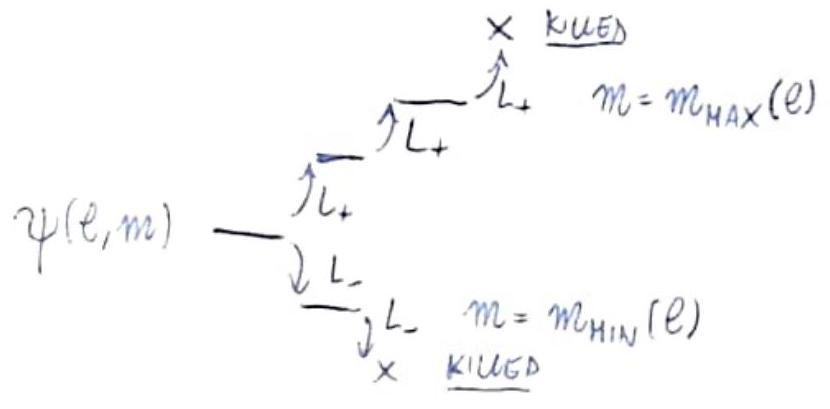
\includegraphics[max width=\textwidth, center]{2025_10_16_22329e0f50bdd2511b17g-04}\\
$L+\psi\left(e, m_{\text {HAX }}(e)\right)=0$ BUT\\
$L^{2}=\psi\left(l, m_{\text {HAX }}\right)=\left(L-L_{+}+L_{z}^{2}+\hbar L_{z}\right) \psi$\\
$f(e) \psi\left(e, m_{\text {HAX }}\right)=L_{x} \psi+L_{2}^{2} \psi\left(e, m_{\text {HAX }}\right)+\hbar L_{z} \psi\left(e, m_{\text {HAX }}\right)$

$$
\begin{aligned}
& =\left(\hbar^{2} m_{\text {HAX }}^{2}+\hbar^{2} m_{\text {HAX }}\right) \psi \\
f(e) & =\hbar^{2} m_{\text {HAX }}(e)\left(1+m_{\text {HAX }}(e)\right) \sqrt{ } \operatorname{sinICARCY}
\end{aligned}
$$

$1-\psi\left(e, m_{\text {HIN }}\right)=0$\\
$f(e) \psi\left(e, m_{\text {HIN }}(e)\right)=L^{2} \psi=L_{+} L \gamma\left(l, m_{\text {H } N}\right)+L_{2}^{2} \psi-\hbar L_{z}=\hbar^{2}\left(m_{\text {H } N}-i\right) m_{\text {M } N} \psi$

$$
f(e)=\hbar^{2} m_{\text {MIN }}\left(m_{\text {HIN }}-1\right)
$$

SYSTET $\left\{\begin{array}{l}m_{\text {HAX }}\left(m_{\text {HAX }}+1\right)=m_{\text {HIN }}\left(m_{\text {MIN }}-1\right) \\ m_{\text {MAX }}-m_{\text {MIN }}=\frac{\hbar}{\hbar} N\end{array}\right.$

\section*{SOUTTION}
$$
\left\{\begin{aligned}
m_{\text {HAX }}= & \begin{array}{r}
\text { POSITIVE INTEGER } \\
\text { TOS, HALF INTEGER }
\end{array} \\
m_{\text {HIN }}= & -m_{\text {MAX }}
\end{aligned}\right.
$$

FROM NOW EN, WE LABEL $l=m_{\text {HAX }}$

$$
\begin{aligned}
& L_{-}^{2} \psi(l, m)=\hbar^{2} l(l+1) \psi(l, m) \\
& L_{z} \psi(l, m)=\hbar m \psi(l, m)
\end{aligned}
$$

$$
f(e)=\hbar^{2} e(e+1)
$$

WHERE $l \in \frac{\mathbb{N}}{2}$ AND $\quad m \in\{-l, \ldots,+l\}$\\
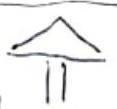
\includegraphics[width=0.5\textwidth, center]{2025_10_16_22329e0f50bdd2511b17g-05}

However, these ruces simply foulow from the algebra structure

$$
\left[A_{i}, A_{j}\right]=i \hbar \varepsilon_{i j k} A_{k}
$$

and use no other information. even the "internal hagentic bipole moment" (aka spin) obeys these rules.\\
4.T THE OrbITAL angular momentum has more structure\\
$\vec{L}=\vec{r} \times \vec{p}$ WHICH IMPOSES FURTHER RESTRICTIONS

\section*{TRICK}
$L_{z}=r_{x} p_{y}-r_{y} p_{x}$\\
$r_{1}^{2}-r_{2}^{2}=2 r_{x} p_{y}$\\
$p_{1}^{2}-p_{2}^{2}=-2 r_{y} p_{x}$\\
THUS\\
$L_{z}=\underbrace{\frac{1}{2}\left(r_{1}^{2}+p_{1}^{2}\right)}_{\substack{\text { GUANY } \\ \text { HANY. } \\ \text { OSCICT } \\ H_{1}}}-\underbrace{\frac{1}{2}\left(r_{2}^{2}+p_{2}^{2}\right)}_{\substack{\text { ANT } \\ \text { ONE }}}$\\
$\left[L_{z}, H_{1}\right]=\left[L_{z}, H_{2}\right]=0$

$$
\left[H_{1}, H_{2}\right]=0
$$

$$
L_{z}=H_{1}-H_{2} \quad \hbar m \psi=L_{z} \psi=\hbar\left(\left(n_{1}+\frac{1}{2}\right)-\left(n_{2}-\frac{1}{2}\right)\right) \psi
$$

$$
\left.\begin{array}{c}
m=n_{1}-n_{2} \\
\stackrel{\leftarrow}{\mathbb{Z}} \\
\stackrel{\vdots}{\in \mathbb{Z}}
\end{array}\right\} \quad m \in \mathbb{Z} \rightarrow e \text { INTEGER! }
$$

But oncy when $\vec{L}=\vec{r} \times \vec{p}$\\
is arbital is orbital

Why is This Important?\\
$\left.\operatorname{AS}_{\text {SALD }} \omega E\right) \rightarrow-\frac{\hbar^{2}}{2 m}\left(\frac{1}{r^{2} \sin \theta} \frac{\partial}{\partial \theta}\left(\sin \theta \frac{\partial}{\partial \theta}\right)+\frac{1}{r^{2} \sin ^{2} \theta} \frac{\partial^{2}}{\partial \varphi^{2}}\right)=\frac{|L|{ }^{2}}{2 m r^{2}}$\\
$H=\underbrace{-\frac{\hbar^{2}}{2 m}\left(\frac{1}{r^{2}} \frac{\partial}{\partial r}\left(r^{2} \frac{\partial}{\partial r}\right)\right)+V_{\text {CORE }}(r)}_{\text {OVY RADIAL }}+\frac{\left|L^{2}\right|}{2 m r^{2}}$

$$
\begin{gathered}
{\left[r, L^{2}\right]=\left[\frac{\partial}{\partial r}, L^{2}\right]=0} \\
\omega=0 \\
{\left[H, L^{2}\right]=0}
\end{gathered}
$$

\begin{center}
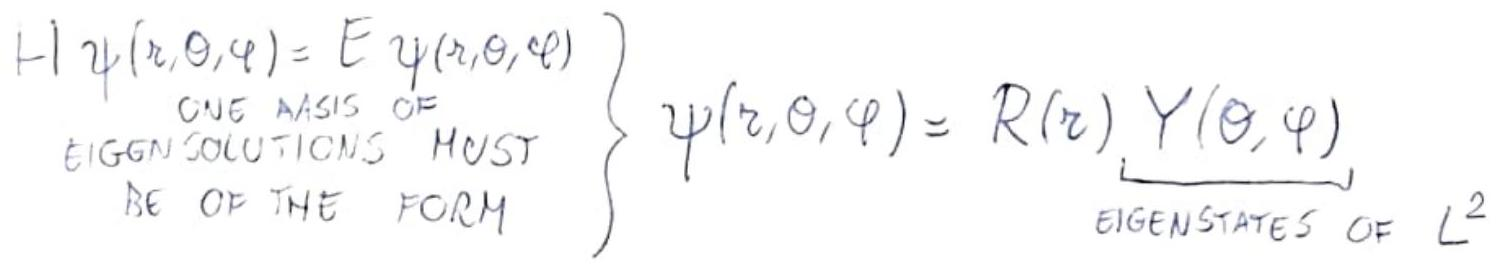
\includegraphics[width=0.5\textwidth]{2025_10_16_22329e0f50bdd2511b17g-06}
\end{center}

\section*{Angular Momentum un Polar Coordinates}
$(\hat{x}, \hat{y}, \hat{z}) \longrightarrow(\hat{r}, \hat{\theta}, \hat{\varphi})$\\
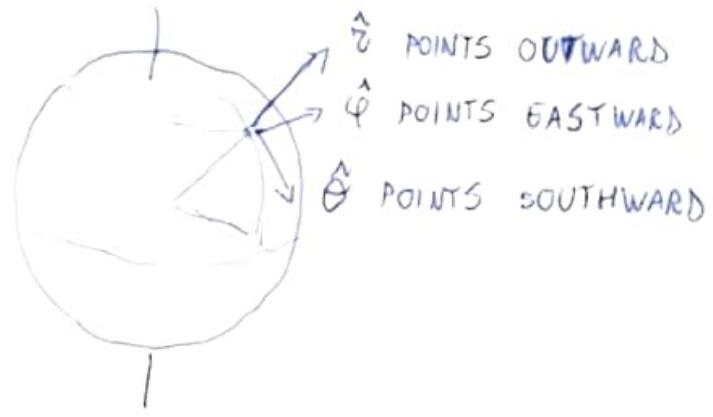
\includegraphics[width=0.5\textwidth, center]{2025_10_16_22329e0f50bdd2511b17g-07}

$$
\hat{r}=\left(\begin{array}{c}
\sin \theta \cos \varphi \\
\sin \theta \sin \varphi \\
\cos \theta
\end{array}\right) \quad \hat{\theta}=\left(\begin{array}{c}
\cos \theta \cos \varphi \\
\cos \theta \sin \varphi \\
-\sin \theta
\end{array}\right) \quad \hat{\varphi}=\left(\begin{array}{c}
-\sin \varphi \\
\cos \varphi \\
0
\end{array}\right)
$$

\section*{GRASIENT}
$$
\vec{\nabla}=\hat{r} \frac{\partial}{\partial r}+\hat{\theta} \frac{1}{r} \frac{\partial}{\partial \theta}+\hat{\varphi} \frac{1}{r \sin \theta} \frac{\partial}{\partial \varphi}
$$

$\left\{\begin{array}{c}\text { ANGULAR } \\ \text { MOMENTUM }\end{array}\right\} \vec{L}=\vec{r} \times \vec{p}=r \hat{r} \times(-i \hbar) \vec{\nabla}=$

$$
\begin{aligned}
& =-i \hbar\left(\hat{r} \times r^{2} r \frac{\partial}{\partial r}+\hat{r} \times \hat{\theta} r \frac{1}{r} \frac{\partial}{\partial \theta}+\hat{r} \times \hat{\varphi} \frac{r}{r \sin \theta} \frac{\partial}{\partial \varphi}\right) \\
\vec{L} & =-i \hbar\left(\hat{\varphi} \frac{\partial}{\partial \theta}-\hat{\theta} \frac{1}{\sin \theta} \frac{\partial}{\partial \varphi}\right)\left(\neq \begin{array}{c}
r \text { HAS } \triangle I S A P E C A R E D \\
\text { ANGULAR } \\
\text { ACTS ON ANGULES, ONC }
\end{array}\right.
\end{aligned}
$$

(EXAPPLE) $L_{z}=\hat{z} \cdot \vec{L}=-i \hbar\left(\hat{z} / \hat{\varphi} \frac{\partial}{\partial \theta}-\hat{z} \cdot \hat{\theta} \frac{1}{\sin \theta} \frac{\partial}{\partial \varphi}\right)=+i \hbar \frac{(-\sin \theta)}{\sin \theta} \frac{\partial}{\partial \varphi}$

$$
L_{z}=-i \hbar \frac{\partial}{\partial \varphi} \quad\left\{\begin{array}{l}
\varphi \rightarrow \text { ANGLE AROUND THE } z \text {-AXIS } \\
L_{z} \rightarrow \text { DERIVATIVE W/RESPECT TO } \varphi
\end{array}\right.
$$

$\xrightarrow{\text { NOTTKE }}$ STATES WITH $m=0$

STATES WITH几者0

$$
\underset{\text { CONSTNNT IN }}{Y(\theta, \varphi)}=\underset{0}{Y(\theta)} \rightarrow \frac{\partial}{\partial \varphi} Y(\theta)=0_{0}^{\nabla}
$$

$$
Y(\theta, \varphi)=\tilde{Y}(\theta) e^{i m \varphi} \rightarrow i \hbar \frac{\partial}{\partial \varphi} Y(\theta, \varphi)=\hbar m Y
$$

(SIMILARCIY) $L_{x}=-i \hbar(\overbrace{\hat{x} \cdot \hat{\varphi}}^{-\sin \varphi} \frac{\partial}{\partial \theta}-\overbrace{\hat{x} \cdot \hat{\theta}}^{\cos \theta \cos \varphi} \frac{1}{\sin \theta} \frac{\partial}{\partial \varphi})=$

$$
\begin{aligned}
& =i \hbar\left(\sin \varphi \frac{\partial}{\partial \theta}+\cot \theta \cos \varphi \frac{\partial}{\partial \varphi}\right) \\
L_{y} & =i \hbar\left(-\cos \varphi \frac{\partial}{\partial \theta}+\cot \theta \sin \varphi \frac{\partial}{\partial \varphi}\right)
\end{aligned}
$$

(AND THUS)


\begin{align*}
& L_{+}=L_{x}+i L_{y}=i \hbar\left(\cot \theta(\cos \varphi+i \sin \varphi) \frac{\partial}{\partial \varphi}+(\sin \varphi-i \cos \varphi) \frac{\partial}{\partial \theta}\right) \\
& =i \hbar\left(\cot \theta e^{i \varphi} \frac{\partial}{\partial \varphi}+(-i) e^{i \varphi} \frac{\partial}{\partial \theta}\right) \quad \text { ANACARCY FOR } L_{-} \\
& L_{ \pm}=i \hbar e^{ \pm i \varphi}\left(\cot \theta \frac{\partial}{\partial \varphi} \pm(-i) \frac{\partial}{\partial \theta}\right) \\
& L_{-} L_{+}=-\hbar^{2} e^{-i \varphi}\left(\cot \theta \frac{\partial}{\partial \varphi}+i \frac{\partial}{\partial \theta}\right) e^{i \varphi}\left(\cot \theta \frac{\partial}{\partial \varphi}-i \frac{\partial}{\partial \theta}\right)= \\
& \text { USING }\left(\left\{\frac{\partial}{\partial \varphi} e^{i \varphi}=e^{i \varphi}\left(i+\frac{\partial}{\partial \varphi}\right)\right)\right. \\
& =-\hbar^{2} e^{-i \varphi} e^{i \varphi}\left(\cot \theta\left(i+\frac{\partial}{\partial \varphi}\right)+i \frac{\partial}{\partial \theta}\right)\left(\cot \theta \frac{\partial}{\partial \varphi}-i \frac{\partial}{\partial \theta}\right)= \\
& =-\hbar^{2}\left[\cot ^{2} \theta\left(i \frac{\partial}{\partial \varphi}+\frac{\partial^{2}}{\partial \varphi^{2}}\right)+\cot \theta \frac{\partial}{\partial \theta}-i \cot \theta \frac{\partial^{2}}{\partial \theta \partial \varphi}+i \cot \theta \frac{\partial^{2}}{\partial \theta \partial \varphi}+\frac{\partial^{2}}{\partial \theta^{2}}\right. \\
& \text { USING 》) } \left.\frac{\mu}{\sin \theta} \frac{\partial}{\partial \theta}\left(\sin \theta \frac{\partial}{\partial \theta}\right)=\cot \theta \frac{\partial}{\partial \theta}+\frac{\partial^{2}}{\partial \theta^{2}}-\frac{i}{\sin ^{2}} \frac{\partial}{\partial \varphi}\right] \\
& L_{-} L_{+}=-\hbar^{2}\left[\frac{1}{\sin \theta} \frac{\partial}{\partial \theta}\left(\sin \theta \frac{\partial}{\partial \theta}\right)-i \frac{\partial}{\partial \varphi}+\cot ^{2} \theta \frac{\partial^{2}}{\partial \varphi^{2}}\right] \\
& |\vec{L}|^{2}=L_{-} L_{+}+L_{z}^{2}+\hbar L_{z}=(\downarrow)-\hbar^{2} \frac{\partial^{2}}{\partial \varphi^{2}}-i \hbar^{2} \frac{\partial}{\partial \varphi} \\
& L^{2}=-\hbar^{2}\left[\frac{1}{\sin \theta} \frac{\partial}{\partial \theta}\left(\sin \theta \frac{\partial}{\partial \theta}\right)+\frac{1}{\sin ^{2} \theta} \frac{\partial^{2}}{\partial \varphi^{2}}\right] \tag{$\omega$}
\end{align*}


$L_{+}|l, m\rangle=\alpha|l, m+1\rangle \quad$ BuT $\quad \beta=\langle l, m| L_{-}|l, m+1\rangle=\langle l, m+1| L_{+}|h l, m\rangle^{*}=\alpha^{*}$

$$
\begin{aligned}
L_{-} L_{+}|e, m\rangle= & |\alpha|^{2}|e, m\rangle=\left(L^{2}-L_{z}^{2}-\hbar L_{z}\right)|e, m\rangle=\left(e(e+1)-m^{2}-m\right) \hbar^{2}|e, m\rangle \\
& \alpha=\hbar \sqrt{e(e+1)-m(m+1)} e^{i \phi} Z_{\text {THIS PHASE CAN SE SET TO }} \text { ZERO }
\end{aligned}
$$

$\left[L^{2}, L_{z}\right]=0$ common eigengasis but $L_{z}$ acts only on $\varphi$

$$
\begin{aligned}
& L_{z} \psi(\theta, \varphi)=-i \hbar \frac{\partial}{\partial \varphi} \psi(\theta, \varphi) \rightarrow Y_{e, m}(\theta, \varphi)=\left.\tilde{Y}_{e m}(\theta) e^{i m \varphi} m \in\right|_{-e} ^{e} \\
& \psi_{e, m=e}(\theta, \varphi)=Y_{e, e}(\theta) e^{i \ell \varphi} \quad \underbrace{\substack{\text { max w } \\
m=e}} \\
& L+\psi_{e, e}=0 \nabla_{0}^{\nabla} \quad \hbar e^{i \varphi}\left(\frac{\partial}{\partial \theta}+i \cot \theta \frac{\partial}{\partial \varphi}\right) \widetilde{Y}_{e e}(\theta) e^{i e \varphi}=0 \\
& \left(\frac{\partial}{\partial \theta}+i \cot \theta\left(\frac{\partial}{\partial \varphi} e^{i e \varphi}\right)\right) \tilde{Y}_{e e}(\theta)=0 \\
& \theta \in[0, \pi] \\
& \text { Fi! Solution } \forall e l \\
& \mathrm{~N}_{0}, 4 \\
& e^{i \ell \varphi}\left(\frac{\partial}{\partial \theta}-e \cot \theta\right) \widetilde{Y}_{e e}(\theta)=0 \stackrel{\substack{\text { Differential } \\
\text { EQUATION } \\
\text { SOLUTION }}}{\tilde{Y}_{e e}(\theta) \propto \sin ^{l}(\theta)} \\
& \underset{\longrightarrow}{\text { Normalization }} \int e^{-i l \varphi} \sin ^{e} \theta e^{+i l \varphi} \sin ^{e} \theta(d \varphi \sin \theta d \theta)=2 \pi \int_{0}^{\pi} \sin ^{2l+1}(\theta) d \theta \\
& =2 \pi \int_{-1}^{1}(1-\mu)^{e} d \mu=\binom{\text { TRY } M A T}{\text { HOME }}=\frac{4 \pi 2^{2 e}(e!)^{2}}{(2 e+1)!} \\
& Y_{e e}(\theta, \varphi)=\underset{\substack{\text { CHOOSEA } \\
\text { PHASE }}}{(-1)^{e}}\left(\frac{(2 e+1)!}{4 \pi}\right)^{1 / 2} \frac{1}{2^{e} e!} \sin ^{e}(\theta) e^{i e \varphi} \\
& \left\{\begin{array}{ll}
\text { FIND THE } & \text { PHASE } \\
\text { OTHER } & \text { Ye, M }
\end{array} \quad L_{-}|e, m\rangle=\sqrt{\text { elet }+1 \text {-m(m-1) }}|e, m-1\rangle\right. \\
& Y_{e, m-1}=\frac{-\hbar e^{-i \phi}}{\sqrt{e(e+1)-m(m-1)}}\left(\frac{\partial}{\partial \theta}-i \cot \theta \frac{\partial}{\partial \varphi}\right) Y_{e, m}(\theta, \varphi)
\end{aligned}
$$

Spherical Hormonics

table of afew s.m.

$$
\left.Y_{0,0}(\theta, \varphi)=\sqrt{\frac{1}{4 \pi}} \quad\right\} \text { S orbital "SHAR p" }
$$

могинице $\quad \int\left|Y_{\text {ем }}(\theta, \varphi)\right|^{2} \sin \theta d \theta d \varphi=1$

P orbital\\
"PRINCIPAL" BRIGHTEST LINES in FIOMIC SPECTRA OF AUKACI "DIFFUSE"

D crbital wibe fine structure\\
$Y_{20}(\theta, \varphi)=\frac{1}{4} \sqrt{\frac{5}{\pi}}\left(3 \cos ^{2} \theta-1\right)$

$$
\begin{aligned}
& Y_{2-1}=\ldots \quad \sin \theta \cos \theta e^{-i \varphi} \\
& Y_{2-2}=\ldots \quad \sin ^{2} \theta e^{-2 i \varphi}
\end{aligned}
$$

The radial part

$$
\begin{aligned}
& \psi(r, \theta, \varphi)=R(r) Y_{\text {em }}(\theta, \varphi) \quad H \psi=E \psi \\
& \left.R(r)=\frac{\hbar^{2}}{2 m} \frac{1}{r^{2}} \frac{\partial}{\partial r}\left(r^{2} \frac{\partial}{\partial r}\right)+\left[V_{\text {core }}(r)+\frac{\hbar^{2} e(e+1)}{2 m r^{2}}\right]\right) R(r)=E R(r) \\
& \left.\left.=\frac{1}{r^{2}} \frac{\partial}{\partial r}\left(r^{2} \frac{\partial}{\partial r}\right) \frac{P(r)}{r}=\frac{1}{r^{2}} \frac{\partial}{\partial r}\left(r \frac{\partial P}{\partial r}-P\right)=\frac{1}{r^{2}}\left(\frac{\partial P}{\partial r}+r \frac{\partial P}{\partial r}-\frac{\partial^{2} P}{\partial r^{2}}\right)\right)=\frac{\partial P}{\partial r}\right)=\frac{1}{r} \frac{\partial^{2}}{\partial r^{2}} P
\end{aligned}
$$

$$
\begin{aligned}
& Y_{3 m} \rightarrow F \text { ORBITAL } \\
& \text { FEW CRAZY EXPERIMENTAUSTS } \\
& \text { GO BEYONS } \log \text { FOR SANITY } \\
& \text { REASONS. }
\end{aligned}
$$

"FOORTH" or "FUNDAMENTAL"\\
$H \psi=E \psi$ 鸟, radial kinetic

$$
\left(-\frac{\hbar^{2}}{2 m} \frac{\partial^{2}}{\partial r^{2}}+\operatorname{Veff}\right) P(r)=E P(r)
$$

where $V_{\text {eff }}=+\frac{\hbar e(e+1)}{2 m r^{2}}-\frac{\left(Z_{\text {eff }}\right) e^{2}}{4 \pi \varepsilon_{0} r}$\\
7 angular kinetic $\frac{L^{2}}{2 I}, I=m r^{2}$\\
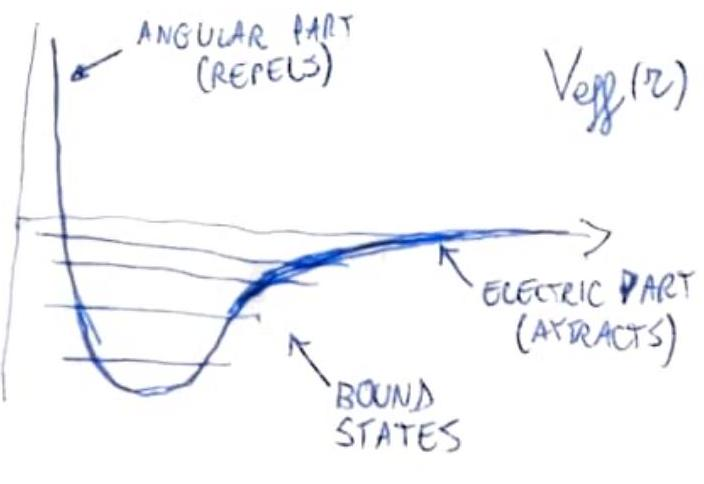
\includegraphics[width=0.5\textwidth, center]{2025_10_16_22329e0f50bdd2511b17g-11(1)}

SOLUTIONS CAN SEPENS ON I BUT NOT $m$

ACTUALUY\\
Hydrogen

\begin{figure}[h]
\begin{center}
\captionsetup{labelformat=empty}
\caption{Hydrogen}
  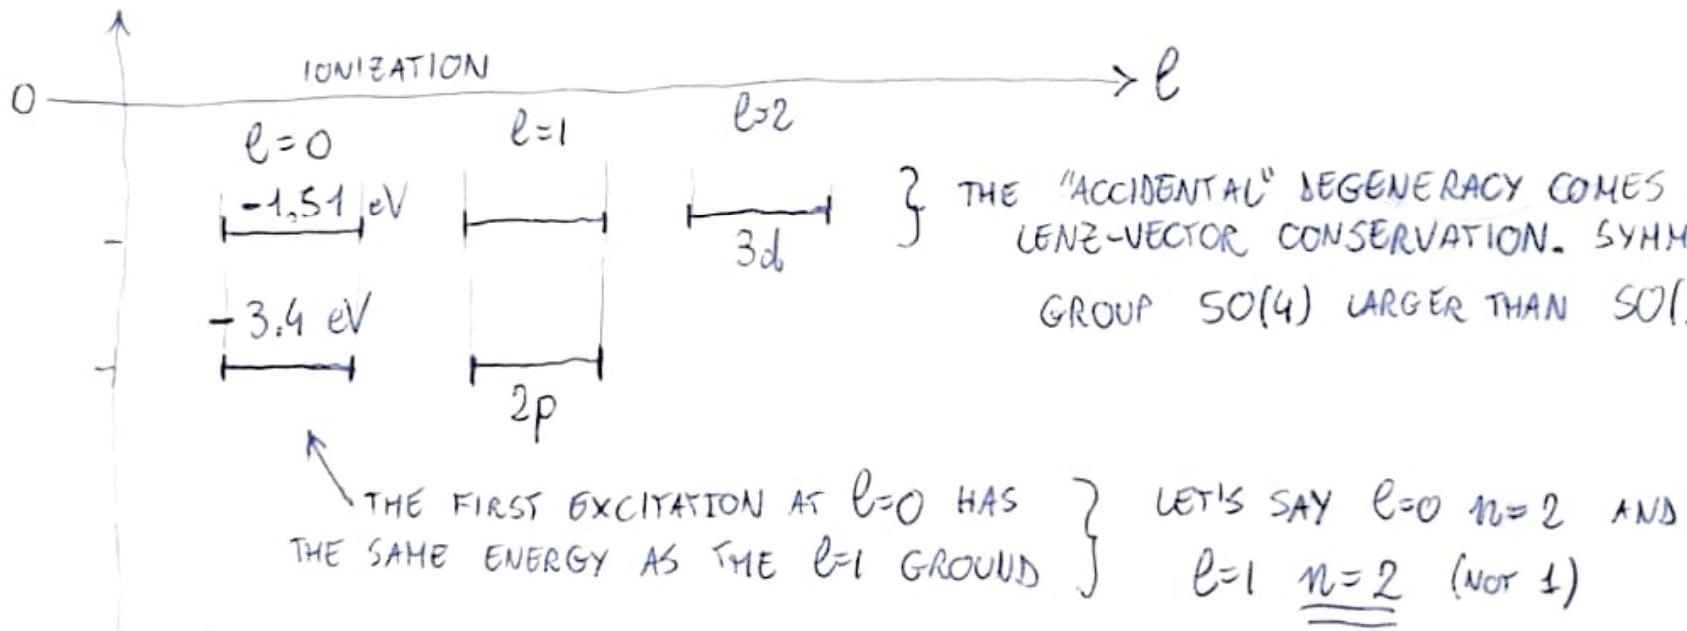
\includegraphics[width=\textwidth]{2025_10_16_22329e0f50bdd2511b17g-11(2)}
\end{center}
\end{figure}

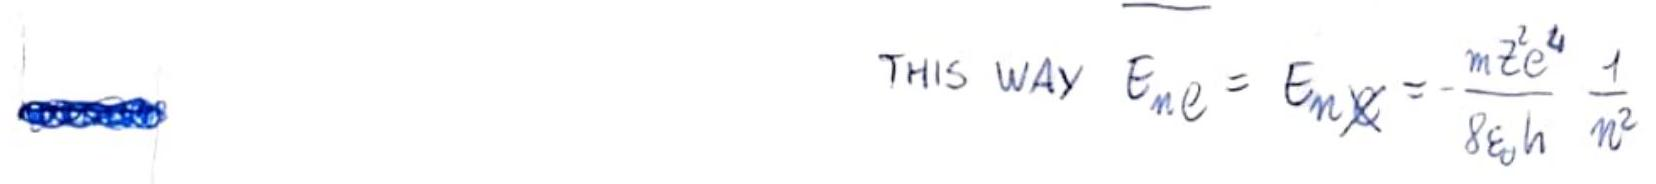
\includegraphics[width=0.5\textwidth, center]{2025_10_16_22329e0f50bdd2511b17g-11}\\
$\left.\frac{-13.6 \mathrm{eV}}{1 \mathrm{~s}} \leftarrow \begin{array}{l}\text { THE ground state } \\ \text { MAS } \quad l=0\end{array}\right\}$ LET'S say $n=1$\\
$\rightarrow$ In THIS NOTATION $l$ gues FROM 0 TO 1 - 1 ; BUT IT'S RATHER $\eta$ GOES FROM $C+1$ TO $\infty$, AND THE ENERGY DEPENDS ONLY ON $\eta$

Other alkall do not have the extra symmetay so the degeneracy is removes Eme, bot we use the same labeling conventons is removes Eme, but we use the same cabeling conventons

Ather Alkau - example: Sodum

$$
\begin{aligned}
H= & \sum_{j}^{\text {elec. }}\left(-\frac{\hbar^{2}}{2 m} \nabla_{j}^{2}-\frac{Z e^{2}}{4 \pi \varepsilon_{0} r_{j}}\right)+\sum \frac{e^{2}}{4 \pi \varepsilon_{0}\left|\vec{r}_{j}-\vec{r}_{j}\right|} \quad \text { Not SOUVABLE } \\
& \left.\frac{\text { GOOD APPROXIMATION }}{\text { HARTREE-FOCK }}\right\} \quad \begin{array}{l}
\text { NO CORRELATIONS/ENTANGLEMENT } \\
\rightarrow \text { ELEETIONG OCCUPY ORTHOGONAL ORBITALS } \\
\rightarrow \text { MINIMIZE ENERGY FUNCTIONAL OVER ORBITALS }
\end{array}
\end{aligned}
$$

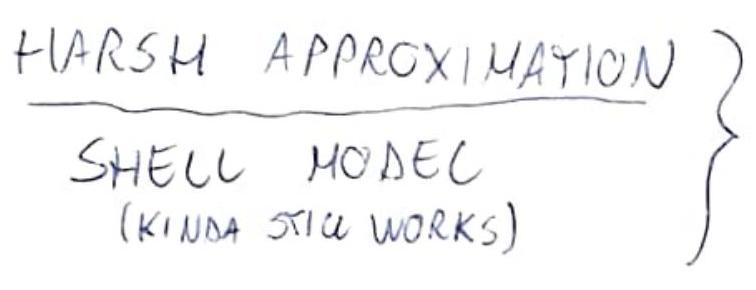
\includegraphics[width=0.5\textwidth, center]{2025_10_16_22329e0f50bdd2511b17g-12(2)}\\
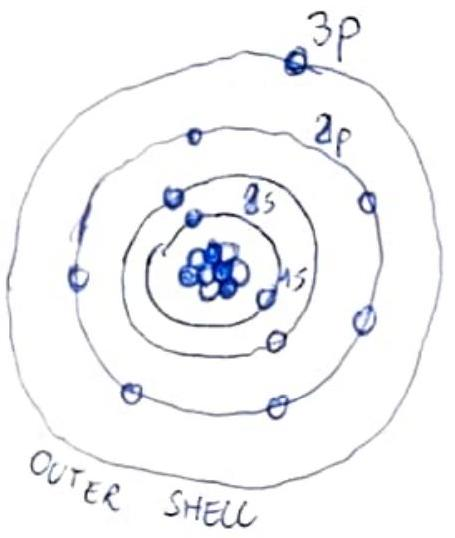
\includegraphics[width=0.5\textwidth, center]{2025_10_16_22329e0f50bdd2511b17g-12(1)}\\
$\rightarrow$ First, ELECTRONS FIU AN ATOMIC SHELL ( 2 (e+1) electrons in an eorsital)\\
$\rightarrow$ THEN, THEY SCREEN THE POETENTIAC\\
$\rightarrow$ REPEAT UNTIL NO MORE ELECTRONS

COTER SHELL EXPERIENCES \~{}HYDROGEN BUT MORE ATYRACTVE ccose to the core\\
\~{}HIGHER e PUSH e- ANNAY FROM THE CORE $\rightarrow$ LESS SHIFT\\
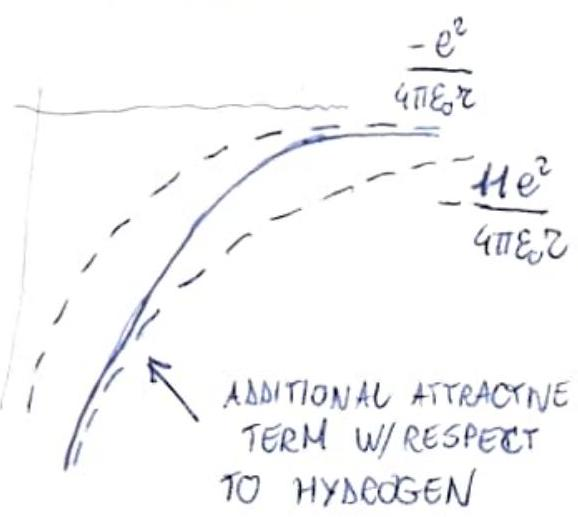
\includegraphics[width=0.5\textwidth, center]{2025_10_16_22329e0f50bdd2511b17g-12(3)}\\
thus, the 11th-electron of sodium sees the core as "acmost" a hydrogen, but not quite\\
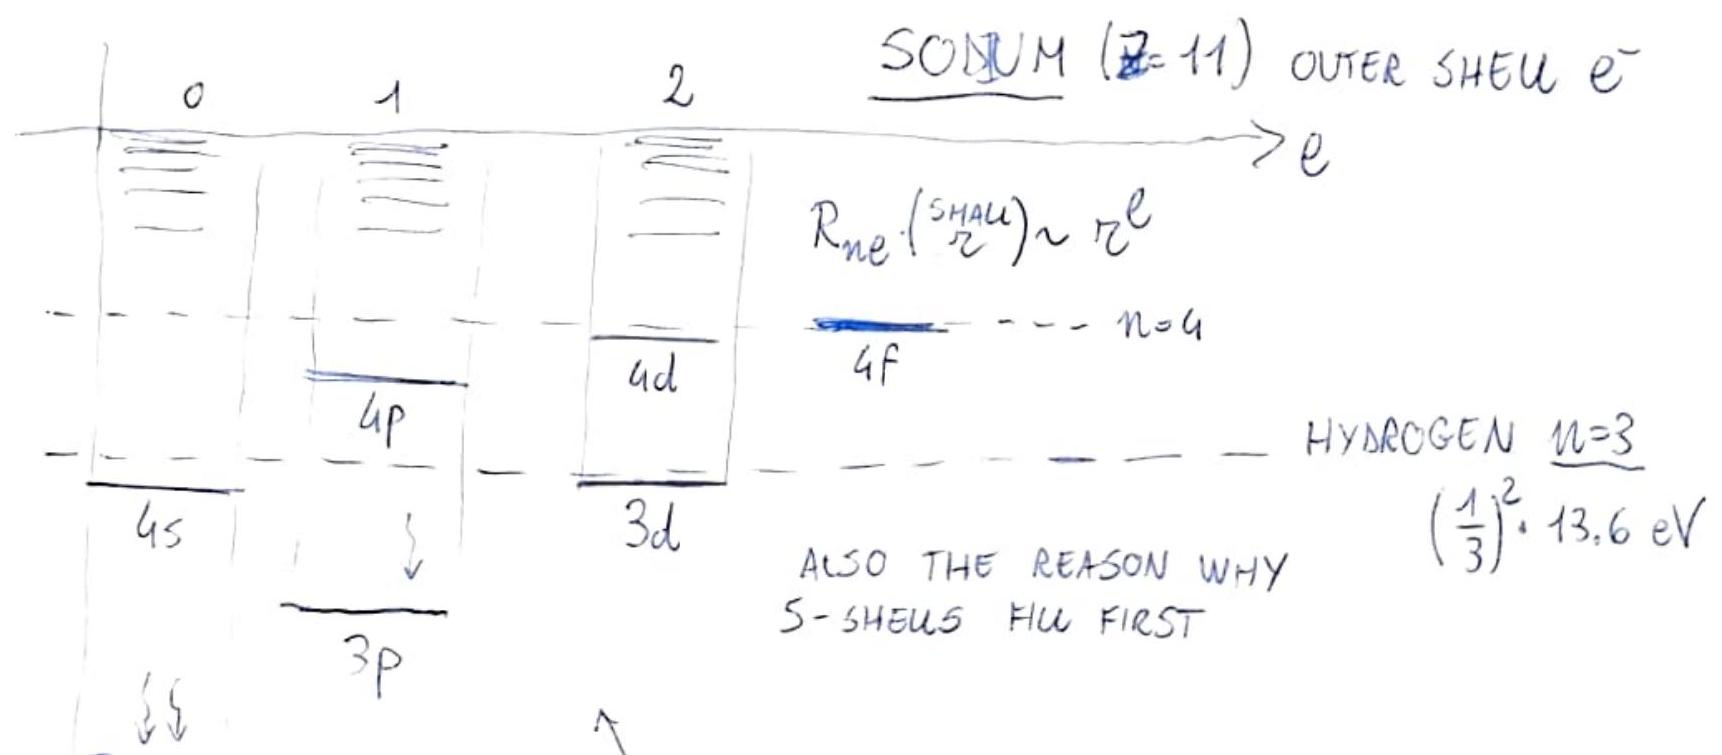
\includegraphics[width=0.5\textwidth, center]{2025_10_16_22329e0f50bdd2511b17g-12(4)}\\
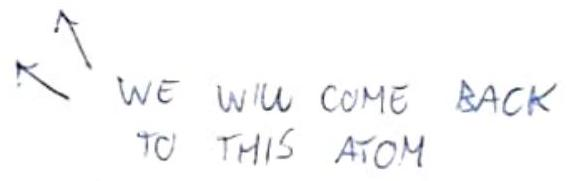
\includegraphics[width=0.5\textwidth, center]{2025_10_16_22329e0f50bdd2511b17g-12}

\section*{Dipole Transitions}
\begin{center}
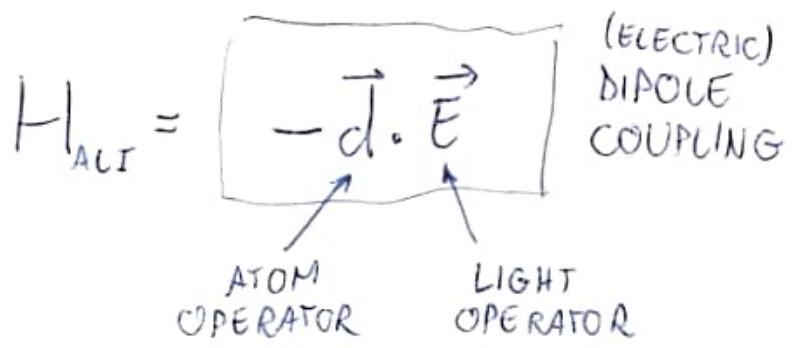
\includegraphics[width=0.5\textwidth]{2025_10_16_22329e0f50bdd2511b17g-13(1)}
\end{center}

FOR AN ALKACI ATOM\\
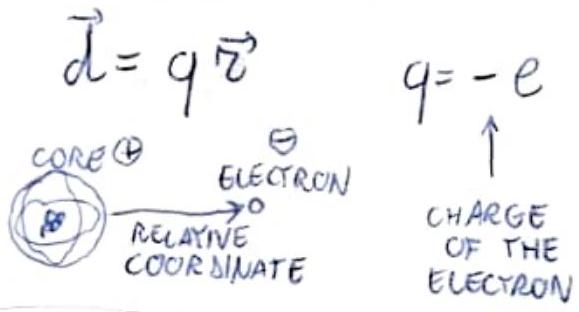
\includegraphics[width=0.5\textwidth, center]{2025_10_16_22329e0f50bdd2511b17g-13(2)}\\
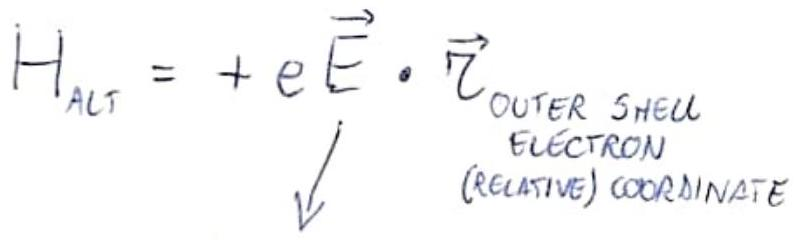
\includegraphics[width=0.5\textwidth, center]{2025_10_16_22329e0f50bdd2511b17g-13}\\
vector in the drectlon of dolarization $\vec{\epsilon}_{K \lambda}$

REFRESHER $\rightarrow$ CLASBICAL DIPOLE\\
$\left.\begin{array}{l}\underset{d}{d}+q \\ \underset{d-q}{d}\end{array}\right\} \begin{gathered}\text { IS a } \triangle P O L E \quad \begin{array}{l}Q+q \\ T a / 2\end{array} \\ \text { THUS }\end{gathered}+\begin{gathered}T-\pi / 2 \\ V-q\end{gathered}$\\
$\hat{I}|q \vec{d}|$ in diefction $+\hat{d}$

We must understand how $\vec{r}$ acts as an operator on ATOMIC LEVELS $\mid N, l, M, \ngtr>$ (electron spin has no el. DI POLE)\\
FACT 1, NO DIAGONAL COMPONENT

$$
\langle n, l, m| \vec{r}|n, l, m\rangle=0
$$

(PRCOF) $\hat{R}$ "PRANTY TRORHATION $\approx \hat{R} \psi(x, y, z)=\psi(-x,-y,-z)$\\
$\tilde{R} \hat{\vec{r}} \tilde{R}^{+}=-r$

$$
\stackrel{s}{R} \psi(r, \theta, \varphi)=\psi(r, \pi-\theta, \varphi+\pi)
$$

$$
\left\{\begin{array}{c}
\mathbb{V} \\
\{\hat{\vec{r}}, \tilde{R}\}=0
\end{array}\right.
$$

$\square \tilde{R}\left(R_{h e}(r) Y_{e_{m}}(\theta, \varphi)\right)=(-1)^{e} R_{n e} Y_{e_{m}}$ WHy?

$$
\begin{aligned}
Y_{e e} & =\sin ^{e}(\theta) e^{i l \varphi} \\
\tilde{R} Y_{e l} & =\sin ^{e}(\pi-\theta) e^{i l(\varphi+\pi)}=e^{i l \pi} e^{i l \varphi} \sin ^{e}(\theta) \\
& =e^{i l \pi} Y_{e l}=(-1)^{e} Y_{e l}
\end{aligned}
$$

$\operatorname{But}_{\text {ALSO }}\left[\tilde{R}, L_{ \pm}\right]=0 \quad[\tilde{R}, \vec{L}]=0 \Leftrightarrow \vec{L}$ WA A

$$
\begin{aligned}
\vec{L}=\vec{r} \times \vec{p} \sim[\tilde{R}, \vec{r} \times \vec{p}] & =\tilde{R} \vec{r} \times \vec{p}-\vec{r} \times \vec{p} \tilde{R} \\
& =(-\vec{r} \tilde{R}) \times \vec{p}-\vec{r} \times(-\tilde{R} \vec{p})=0
\end{aligned}
$$

THEREFORE $\tilde{R} Y_{e-i}(\theta, \varphi)=\frac{1}{\sqrt{e(e+1)-e(e-i)}} \tilde{R} L-Y_{ee}(\theta, \varphi)=$\\
$=\frac{1}{\sqrt{\ldots}} L \cdot \tilde{R} Y_{ee}=\frac{(-1)^{e}}{\sqrt{-}} L-Y_{ee}(\theta, \varphi)=(-1)^{e} Y_{e, l-1}(\theta, \varphi)$

AND BY RECURSION IT WORKS FOR ANY m

BUT NOW CONSIDER

$$
\begin{aligned}
& \langle n, l, m| \vec{r}|n, l, m\rangle=\langle n, l, m| \underbrace{R^{+} R}_{\text {DENTIY }} \vec{r}|n, l, m\rangle= \\
& =-\langle n, l, m| R^{+} \vec{r} R|n, l, m\rangle=-(-1)^{l}\langle n, l m| \vec{r}|n l m\rangle(-1)^{l}= \\
& \text { nons }
\end{aligned}
$$

FACT 2, selection Rule on $l$\\
we start from a (not neoven) equation

$$
\left[L^{2},\left[L^{2}, \vec{r}\right]=2 \hbar^{2}\left\{\vec{r}, L^{2}\right\}\right.
$$

\begin{center}
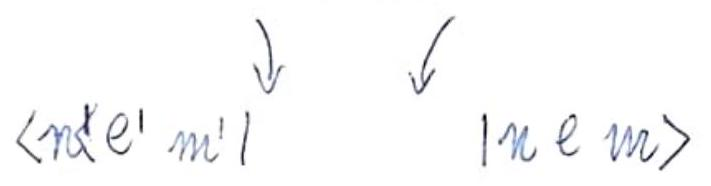
\includegraphics[width=0.5\textwidth]{2025_10_16_22329e0f50bdd2511b17g-14}
\end{center}

THIS CAN BE DEMONSTRATED USING ONCY

$$
\begin{aligned}
& \vec{L}=\vec{r} \times \vec{p} \quad \begin{array}{l}
L^{2}=L_{x}^{2}+L_{y}^{2}+L_{z}^{2} \\
=\vec{L} \cdot \vec{L}
\end{array} \\
& \left\{\tau_{J^{\prime}} p_{T^{\prime}}\right\}=i \hbar \delta_{J^{\prime}} \\
& \text { BUT IT IS SIFFICULT! } \\
& \text { MAYBE AN ASSIGNMENT }
\end{aligned}
$$

$\left\langle n e^{\prime} n n^{\prime}\right|\left(L^{2}\right)^{2} \vec{r}-2 L^{2} r L^{2}+\vec{r}\left(L^{2}\right)^{2}|n e m\rangle=$\\
$2 \hbar^{2}\left\langle n l^{\prime} m^{\prime}\right| \vec{r} L^{2}+L^{2} r|n l m\rangle=$\\
$t^{4}\left(\left[e^{\prime}\left(e^{\prime}+1\right)\right]^{2}-2 e^{\prime}\left(e^{\prime}+1\right) e(e+1)-[e(e+1)]^{2}\right)\left\langle n^{\prime} e^{\prime} m^{\prime}\right| \vec{r}|n e m\rangle=$\\
$2 \hbar^{4}\left(e^{\prime}\left(e^{\prime}+1\right)+e(e+1)\right)\left\langle n^{\prime} e^{\prime} m^{\prime}\right| \vec{r}|n l m\rangle$\\
$O=\left[\left(e^{\prime}\left(e^{\prime}+1\right)-e(e+1)\right)^{2}-2\left(e^{\prime}\left(e^{\prime}+1\right)+e(e+1)\right)\right]\left\langle n^{\prime} e^{\prime} m^{\prime}\right| \vec{r}|n l m\rangle$\\
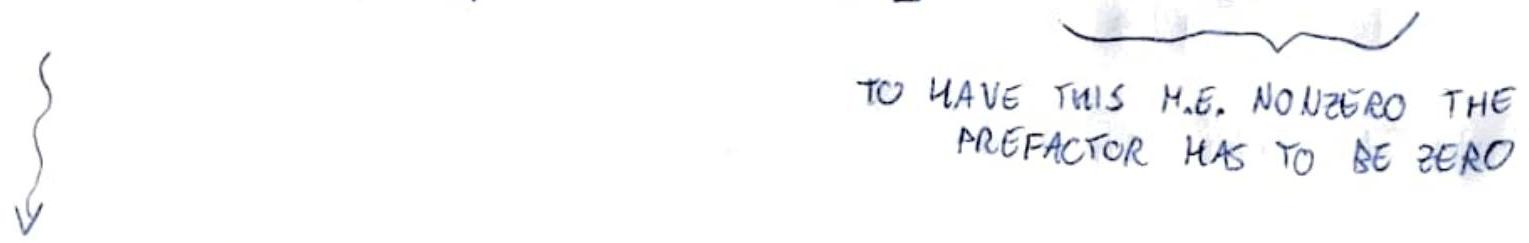
\includegraphics[width=0.5\textwidth, center]{2025_10_16_22329e0f50bdd2511b17g-15}\\
$\underset{\text { (A) }}{\left(e^{\prime}-e+1\right)} \underset{\text { (B) }}{\left(e^{\prime}-e+1\right)} \underset{\text { (C) }}{\left(e+e^{\prime}\right)} \underbrace{\left(e^{\prime}+e+2\right)}_{\text {NEVER ZERO }}$ Wirn $e, e^{\prime} \geqslant 0$

\section*{OPTIONS}
A $\mid e^{\prime}=e+1 \quad \checkmark$ ok\\
B $e^{\prime}=e-1 \quad \checkmark$ ok\\
c $e=e^{\prime}=0$ HOWEVER $\langle n 00| \vec{r}\left|n^{\prime} O 0\right\rangle \quad \begin{gathered}\text { BECAUSE OF PARIYY } \\ \text { ARGUMENT }\end{gathered}$ ARGUMENT\\
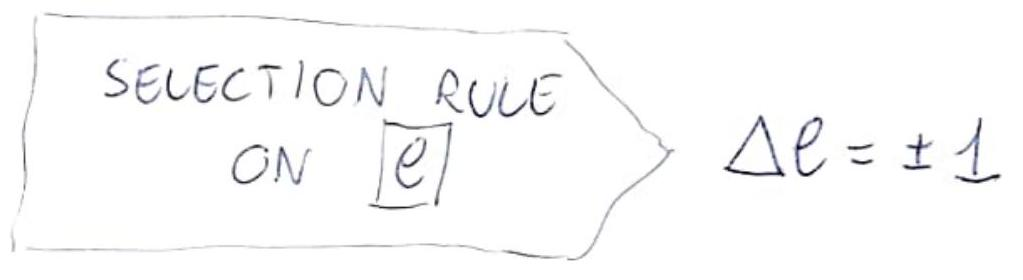
\includegraphics[width=0.5\textwidth, center]{2025_10_16_22329e0f50bdd2511b17g-15(1)}

Fact 3, let's now assume $\vec{E}$ is polarized along $z$-axis\\
$L_{z} \cdot|e, m\rangle=\hbar m$ and $L_{z}=r_{x} p_{y}-r_{y} p_{x}$\\
clearly $\left[L_{z}, z\right]=0$ cuz $z$ commutes with $r_{x, y} p_{x, y}$\\
$0=\left\langle n^{\prime} l^{\prime} m^{\prime}\right|\left[L_{z}, z\right]|n e m\rangle=$\\
$\left\langle n^{\prime} l^{\prime} m^{\prime}\right|\left(L_{z} z \mid-z L_{z}\right)|n l m\rangle=\hbar\left(m^{\prime}-m\right) \underbrace{\left\langle n^{\prime} l^{\prime} m^{\prime}\right| \hat{z}|n l m\rangle}_{\text {TO HAVE THIS MATRA ELEHENT }}$\\
ON M

$$
\Delta m=0
$$

FACT4 NOW $\vec{E}$ POLARIZES ON $\tilde{x}$ (OR $\hat{y}$ ) AXES

$$
\begin{aligned}
& {\left[L_{z}, x\right]=\left(x p_{y}-y p_{x}\right) x-x\left(x p_{y}-y p_{x}\right)=y\left(x p_{x}-p_{x} x\right)=i \hbar y} \\
& {\left[L_{z}, y\right]=\ldots=-i \hbar x}
\end{aligned}
$$

S

$$
\begin{aligned}
& {\left[L_{z}, x+i y\right]=(i \hbar y)+i(-i \hbar x)=\hbar(x+i y) \quad\left[L_{z}, x-i y\right]=-\hbar(x-i y)} \\
& \left\langle n^{\prime} l^{\prime} m^{\prime}\right|\left[L_{z}, x+i y\right]|n e m\rangle=\hbar\left\langle w l^{\prime} m^{\prime}\right|(x+i y)|n e m\rangle
\end{aligned}
$$

$\hbar\left(m^{\prime}-m-1\right)\left\langle n^{\prime} l^{\prime} m^{\prime}\right| x+i y|n l m\rangle=0 \quad$ AND

$$
\hbar\left(m^{\prime}-m+1\right)\left\langle n^{\prime} e^{\prime} m^{\prime}\right| x-i y|n l m\rangle=0
$$

to have $\langle\cdot| x|\cdot\rangle \neq 0$ at least one $\left\langle 0^{\prime}\right| x \pm i y|0\rangle$ hust be nonzero $\rightarrow$

BUT THEN

$$
\begin{aligned}
& m^{\prime}=n+1 \\
& m^{\prime}=m-1
\end{aligned}
$$

Sele ction ROLE ON M xy-plant polarization.

$$
\Delta m= \pm 1
$$

\section*{SODIUM (again)}
\begin{center}
\includegraphics[width=0.5\textwidth]{2025_10_16_22329e0f50bdd2511b17g-16}
\end{center}

% Lecture file created by Gemini
% Class: Quantum Information With Atoms and Photons
% Professor: Pietro Silvi
% Date: 2025-10-16
\lecture{5}{Lifting atom degeneracy}{2025-10-16}

% --- Start writing here ---
\captionsetup{singlelinecheck=false}
Lifting Energy-Level degeneracies in Hydrogen-like atoms

NOU RELATNISTIC $>H=\frac{\vec{p}^{2}}{2 m}+V_{\text {egr }}$ (OUI)

$$
\begin{aligned}
& m \approx m_{e} \quad \text { RESUCES MASS } \\
& {\left[T_{3}, P_{1}\right]=i \hbar \delta_{11} \quad \text { RESOCES }} \\
& \text { COORS-MOM. }
\end{aligned}
$$

True\\
HYDROGEN\\
energy levels\\
energy levels\\
$V(\Omega)=-\frac{(z=1) e^{2}}{4 \pi \varepsilon_{0}} \frac{1}{2} \quad V(\Omega)=-\frac{(z=1) e^{2}}{4 \pi \varepsilon_{0}}\left(\frac{1}{2}+C(\Omega)\right) \quad V(\Omega)=-\frac{(z=2) e^{2}}{4 \pi \varepsilon_{0}}$\\
$\xrightarrow{\text { ENERGY LEVELS }} E_{n(e)}=-\frac{m_{e} e^{4} z_{k}^{2}}{2\left(4 \pi \varepsilon_{0}\right)^{2} \hbar^{2}}\left(\frac{1}{n^{2}}+\widetilde{\zeta}_{n, e}\right)$\\
$\uparrow \Rightarrow L_{\text {corre ction for }}$\\
COMAARING THIS EXPRESSION TO THE ELECTRON REST ENERGY\\
$E_{n(e)}=-\frac{m c^{2}}{2} Z_{R}^{2}(\underbrace{\frac{e^{2}}{4 \pi \varepsilon_{0} \hbar c}}_{\text {Fine Structure }})^{2}\left(\frac{1}{n^{2}}+\zeta_{n, e}\right)=-\frac{m c^{2}}{2}\left(Z_{R} \alpha\right)^{2}(\ldots)$\\
$n c^{2} \approx m_{e} c^{2}=511 \mathrm{KeV} \rightarrow E_{n=1}^{H \times D A O}=-\frac{511 \mathrm{KeV}}{2(137)^{2}}=-13.6 \mathrm{eV}$\\
$E_{n(e)}^{\text {Hol } \mathrm{k} \mathrm{e} \mathrm{e}}=-\frac{m_{e} c^{2}}{2}\left(Z_{R} \alpha\right)^{2}\left(\frac{1}{n^{2}}+\tilde{e}_{n e}\right)$\\
natural alkal $z_{c}=1$\\
AKKALME-EARTH IONS $z_{R}=2$\\
Lifting the Degenerocy.\\[0pt]
(1) Fine structure arsa. spin-orbit coupung [native perturbation]\\
(2) Eeeman Smitting [external $\vec{B}$ static, can de perturbative]

ACKALINE-EARTH\\
IONS\\
$-\frac{(z=2) e^{2}}{4 \pi \varepsilon_{0}}\left(\frac{1}{2}+c(r)\right)$\\
COREECTION AT\\
SHORT RADII lower $e$\\
states of the outer shell electron\\
\includegraphics[max width=\textwidth, center]{2025_10_16_e34e240cf6beac2f9e0dg-1}

\section*{Fine Structure (a quick outrview) - lowest orser of $\vec{B}$ fields}
\includegraphics[max width=\textwidth, center]{2025_10_16_e34e240cf6beac2f9e0dg-2(1)}\\
NO MAGNETIC FHELS IN LAB FRAME\\
$\downarrow$\\
yes thageetive fleed in é rest frame\\
$\left.\underset{\uparrow}{\vec{B}}=-\frac{1}{C^{2}} \vec{v} \times \vec{E}=\left\lvert\, \begin{array}{c}\text { CORE } \\ \text { ELECTRIC FIELD } \\ \text { IN LAE FRAME } \\ \text { ELECTRON VELOCITY }\end{array}\right.\right\}$ III ITS REST FRDME

THIS COMES FROM delativity + MAXWELL EQS.\\
$\vec{E}$ is radial so

$$
\vec{E}=\frac{\vec{\nabla} V}{-e}=\frac{t \vec{r}}{e|r|} \partial_{r} V_{\text {elf }} / r
$$

$\vec{B}_{\text {tect }}=-\frac{1}{c^{2}}\left(\frac{\vec{P}}{m} \times \vec{r}\right)\left(+\frac{1}{e r} \frac{\partial V_{e r}}{\partial r}\right)$

BUT

$$
\vec{P} \times \vec{r}=-\vec{r} \times \vec{P}=\vec{L}
$$

even in guantuh mechanic\\
$\vec{B}_{\text {FERT }}=\left(+\frac{1}{\text { emc }{ }^{2} r} \frac{\partial V}{\partial r}\right) \vec{L}_{\text {angular momentul in the las frame }}$

How the é spin has a magnetic DIOCE MCMENT ASSOCIATES TO IT\\
\includegraphics[max width=\textwidth, center]{2025_10_16_e34e240cf6beac2f9e0dg-2(2)}\\
A RIGID SYSTEM CF\\
(SPHERICAUY-SISTRIBUTED) massive charges mas

$$
\vec{\mu}=\frac{9}{2 m} \vec{L}
$$

THIS MOULL FALLS FOR THE EECTRON i.i a. FACTOR ge

$$
\sqrt{415} \text { monell }
$$

$$
\vec{\mu}=-\frac{e}{2 m} g_{S} \vec{S}-\text { SPMGUAR }
$$

\begin{center}
\includegraphics[max width=\textwidth]{2025_10_16_e34e240cf6beac2f9e0dg-2}
\end{center}

$$
\begin{aligned}
& \mu_{B}=\frac{e \hbar}{2 m_{e}} \\
& { }_{O R}
\end{aligned}
$$

olectron

$$
g-\text { FACTOR }
$$

\includegraphics[max width=\textwidth, center]{2025_10_16_e34e240cf6beac2f9e0dg-2(3)}\\
3. $2 \frac{\text { FROM SIRAC FREE THEORY }}{\text { VARIA TI⿴囗 ANY FERMION S=1/2 }}>$ CORRECTIONS?\\
\includegraphics[max width=\textwidth, center]{2025_10_16_e34e240cf6beac2f9e0dg-2(4)}

COUPING $\vec{B}$ TO $\vec{\mu}$\\
$H=-\vec{\mu} \cdot \vec{B} \leftarrow$ SO SIMPLE $\} \begin{aligned} & \text { Precession } \\ & \text { HAHICTONIAN }\end{aligned}$\\
\includegraphics[max width=\textwidth, center]{2025_10_16_e34e240cf6beac2f9e0dg-3}\\
$\left.H\left(\begin{array}{c}\text { ELECTRON } \\ \text { REST } \\ \text { FRAME }\end{array}\right)=-\left(-\frac{\mu_{B} g_{S}}{\hbar}\right) \right\rvert\, \vec{S} \cdot\left(\frac{1}{e_{m c^{2}} r} \frac{\partial V}{\partial r}\right) \vec{L}=$\\
$=+\frac{\mu_{B} g_{s}}{e m c^{2} \hbar}\left(\frac{1}{r} \frac{\partial V_{\text {ess }}}{\partial r}\right) \vec{S} \cdot \vec{L}$ HOWEVER, WE NEED TO MOVE EFFECT $\rightarrow g_{S} \xrightarrow[\text { LAB }]{\text { TO }} g_{S}-1$\\
$H\binom{\text { LAB }}{\text { FRAME }}=\frac{\mu_{B}\left(g_{s}-1\right)}{e m c^{2} \hbar}\left(\frac{1}{2} \frac{\partial V_{\text {eff }}}{\partial r}\right) \vec{S} \cdot \vec{L} \quad\left\{\begin{array}{c}\text { PUGGING Hydeo-LIKE } \\ \text { POTENTIAL } \\ Z_{0} e^{2}(1\end{array}\right. V(r)=-\frac{Z_{R} e^{2}}{4 \pi \varepsilon_{0}}\left(\frac{1}{r}+e(r)\right)$\\
\includegraphics[max width=\textwidth, center]{2025_10_16_e34e240cf6beac2f9e0dg-3(1)}\\
$\vec{J}\left(\frac{\text { TOTAL }}{\begin{array}{l}\text { TOLALAR } \\ \text { MOMENTUM }\end{array}}\right)=\vec{L}+\vec{S}$ SUM OF TWO ANGULAR MOMENTUM OPERATOR ALGEBRAS (OR FUSION)

$$
\begin{aligned}
{\left[J_{J}, J_{K}\right]=\left[L_{J}, L_{K}\right]+\left[L_{J}, S_{K}\right]+\left[S_{K}, L_{J}\right]+\left[S_{1}, S_{K}\right]=} & \\
& i \varepsilon_{j K e} L_{e}+i \varepsilon_{jKe} S_{e}=i \varepsilon_{jKe}(L+S)_{e}=i \varepsilon_{jKl}-J_{e}
\end{aligned}
$$

also in angular momentum

PRODUCT BASIS\\
$\left|e, m ; s, s_{z}\right\rangle$\\
$\rightarrow \underset{\text { UPON }}{\text { BASE }} \quad L^{2}, L_{z}, S^{2}, S_{z} \quad \underset{\text { COMUTINE }}{\text { AU }}$\\
$\left.\left(\begin{array}{l}L^{2} \\ L_{z} \\ s^{2} \\ s_{z}\end{array}\right)\left|l, m ; s, s_{z}\right\rangle=1.\right\rangle\left(\begin{array}{c}\hbar^{2} e(e+1) \\ \hbar m \\ \hbar^{2} s(s+1) \\ \hbar s_{z}\end{array}\right)$

FUSION BASIS\\
$|U, S ; J, J z\rangle$\\
$L \xrightarrow[\substack{\text { BASED } \\ \text { UPON }}]{ } L^{2}, S^{2}, J^{2}, J_{z} \quad$ COMHUTING\\
$\left(\begin{array}{l}L^{2} \\ S^{2} \\ J^{2} \\ J_{z}\end{array}\right) 1_{0}>1 .>\left(\begin{array}{c}\hbar^{2} e(e+1) \\ \hbar^{2} s(s+1) \\ \hbar^{2} J(J+1) \\ \hbar J z\end{array}\right)$\\
EXAMPLE $l=2$\\
\includegraphics[max width=\textwidth, center]{2025_10_16_e34e240cf6beac2f9e0dg-4}\\
(2) $\theta_{S_{z}=-1 / 2}^{S_{z}+1 / 2} \quad \begin{gathered}D \times 2=10 \\ 5 \times 2\end{gathered}$\\
il FUSES into $\oplus$ J-SPACES FROM $|l-s|$ TO $l+s \quad l+\frac{1}{2}, l-\frac{1}{2}$\\
\includegraphics[max width=\textwidth, center]{2025_10_16_e34e240cf6beac2f9e0dg-4(1)}

$$
\begin{aligned}
& \text { FIXE) } \\
& \left|e^{\downarrow}, s, J, J_{z}\right\rangle=\sum\left(\mid e, m \cdot s, s^{z}\right) C_{e, m, m, s, n}^{\nu} \\
& \left|J_{1} J_{2}\right\rangle=\sum_{\left.m, s^{z}=J_{z}-m, s^{z}\right\rangle} \mid m s_{z}
\end{aligned}
$$

IT IS EASY TO FIND $\left|J_{\text {NAT }}, J_{\text {MAX }}\right\rangle=\left|e^{+} 5, e^{+}+5\right\rangle$\\
RECAUSE $\quad|j=l+5, j=l+5\rangle=\underset{\text { CHUCE }}{\text { +1 }} \quad\left|m=l, S_{z}=+5\right\rangle$\\
\includegraphics[max width=\textwidth, center]{2025_10_16_e34e240cf6beac2f9e0dg-4(2)}

THEN \$\textbackslash left.\textbackslash longrightarrow \textbackslash begin\{array\}\{c\}\text{FIND THE OTHER} \\
\\
\text{J-SHEU (S) BY} \\


\text{ORTMOGONALIZING}\textbackslash end\{array\}\textbackslash right\} \textbackslash quad\$\begin{tabular}{r}
$\left|J=l+S-1, J_{z}=l+S-1\right\rangle$ \\
$\mid S$ ORTHOCONAL TO \\
$\left|J=l+S, J_{z}=l-S-1\right\rangle$ \\
\end{tabular}$\quad$\begin{tabular}{r}
$|N S| \Delta E$ THE SDACE \\
$|m=l, S=S-1\rangle$, \\
$|m=l-1, S z=S\rangle$ \\
\end{tabular}

$\rightarrow$ eventuately repeat\\
(NOT NEEDES FOR $s=1 / 2$ )

$$
\begin{aligned}
& H_{\text {SFAN }}=(\operatorname{STUEF}(r)) \vec{S} \cdot \vec{L} \text { AND } \\
& (\vec{S}+\vec{L})^{2}=J^{2}=S^{2}+L^{2}+\frac{\vec{S} \cdot \vec{L}+L \cdot \vec{S}}{2 \vec{S} \cdot \vec{L}} \quad \vec{S} \cdot \vec{L}=\frac{1}{2}\left(J^{2}-L^{2}-S^{2}\right)
\end{aligned}
$$

$\left.\begin{array}{c}\text { arst order } \\ \text { perturbation }\end{array}\right\} \quad H^{(1)}=\pi_{\text {ne }} H_{\begin{array}{c}\text { spin } \\ \text { orbit }\end{array}} \Pi_{\text {ne }} \quad$ precisely $\quad\binom{\text { siagonal in }}{\text { esjfe }}$

$$
\begin{aligned}
& \Delta E_{\text {sprin }}=\left\langle n e_{j j_{2}}\right| H_{\text {onis }}\left|n e_{j j_{2}}\right\rangle \\
& =\frac{\mu_{s}\left(g_{s}-1\right) \hbar}{2 m c^{2} e}\left\langle n, \left.e_{1}\left(\frac{1}{\eta} \frac{\partial V_{s}}{\partial \eta}\right) \right\rvert\, n, l\right\rangle \underbrace{(J(j+1)}_{\text {POSITIVE }}-\underbrace{\left.\ell(l+1)-\frac{3}{4}\right)}_{\text {SAIT }}
\end{aligned}
$$

Sticl aegenerate in Te

$$
\begin{array}{ll}
l=l+1 / 2 & \operatorname{cose} \frac{U P}{N} \\
\underline{T=l-1 / 2} & \operatorname{coses} \frac{X O W}{N} \\
\hline & \text { in } E N \in R G Y
\end{array}
$$

LABELING LEVELS\\
\includegraphics[width=0.5\textwidth, center]{2025_10_16_e34e240cf6beac2f9e0dg-5(1)}

FOR HYARCHKE $25+1$ is Always 2\\
\includegraphics[width=0.5\textwidth, center]{2025_10_16_e34e240cf6beac2f9e0dg-5}

\begin{figure}[h]
\begin{center}
  \includegraphics[width=\textwidth]{2025_10_16_e34e240cf6beac2f9e0dg-5(2)}
\captionsetup{labelformat=empty}
\caption{EMISSION/ABSORPTION SAECTRUM}
\end{center}
\end{figure}

\begin{figure}[h]
\begin{center}
\captionsetup{labelformat=empty}
\caption{EMISSION/ABSORPTION SAECTRUM}
  \includegraphics[width=\textwidth]{2025_10_16_e34e240cf6beac2f9e0dg-5(3)}
\end{center}
\end{figure}

at this energyscale there are hiso relativistic effects that SHIFT In es RIGIACY. BORNG.

$$
\begin{aligned}
& \text { External, Static Magnetic Fields } \\
& \vec{B} \text { UNIFORH, CONTANT, } \\
& \text { ruasical } \\
& H_{B}=-\vec{\mu}_{s} \cdot \vec{B}-\mu_{L} \cdot \vec{B}=\frac{\mu_{B}}{\hbar}\left(g_{s} \vec{S}+g_{L} \vec{L}\right) \cdot \vec{B} \\
& \begin{array}{l}
\text { SPIN HAGNETIC } \\
\text { OREITALE HAMENT DIPOLE HOMETIC } \\
\text { SIPONT }
\end{array} \\
& \text { DIPOLE HOMENT DIPOLE MOMENT } \\
& g \text {-FACTORS }\left\{\begin{array}{l}
g_{5} \quad \text { SOIN } \quad \text { giaction } \\
g_{c} \quad \text { ORBITAL } \quad g-\text { FACTIOR }=2,0023 \\
\frac{m c}{m_{e}}=\frac{1}{1+m_{e} / m_{\text {CORE }}} \approx 1-\varepsilon
\end{array}\right. \\
& \frac{\text { ROTATE }}{\text { UNTL B1S }} \\
& \text { AUGNCS ACONG } \hat{z} \\
& H_{B}=\frac{\mu_{B}}{\hbar}\left(\sim 2 \xi_{z}+\sim 1 L_{z}^{\infty}\right) B_{z} \quad\binom{\text { TO} D O S}{\text { SLEANRIOS }} \\
& 11 \begin{array}{c}
\text { strong } \\
\text { fields }
\end{array} \\
& \Delta E_{B} \gg \Delta E_{S A I N-O R S I T} \\
& \text { B~1 Tesla } \\
& \text { PASCHEN-BACK eff. } \\
& \text { at this energyscale, ( } m, s_{2} \text { ) are "goos" quantem nuhaers } \\
& \Delta E_{n l m s_{z}}=\left\langle n l m s_{z}\right| H_{B}\left|n l m s_{z}\right\rangle \cong \frac{\mu_{B} B}{\hbar}\left\langle 2 S_{z}+L_{z}\right\rangle
\end{aligned}
$$

$\begin{aligned} & 2 \text { weak } \\ & \text { Zeeman }\end{aligned}$\\
$\Delta E_{B} \backsim \Delta E_{\substack{\text { SPIN } \\ \text { ORBIT }}}$\\
$|n e, j, j z\rangle$\\
at this energyscale, good guantem numbers?\\
wer $\hat{A}_{n}$ elgenuection or $S_{z}$

HOW TO CACCULATE $\left\langle S_{z}\right\rangle$ WE USE THE\\
\includegraphics[width=0.5\textwidth, center]{2025_10_16_e34e240cf6beac2f9e0dg-7(2)}

$$
\begin{aligned}
\left\langle n l_{J J_{z}}\right| S_{z}\left|n l_{J J_{z}}\right\rangle & =\left\langle n l_{J J_{z}}\right|\left(J^{2}\right)^{-1}(\vec{J} \cdot \vec{S}) J_{z}\left|n l_{J J_{z}}\right\rangle= \\
& =\frac{J_{z}}{\hbar J_{J+1}}\left\langle n l_{J J_{z}}\right| \vec{J} \cdot \vec{S}\left|n l_{J J_{z}}\right\rangle
\end{aligned}
$$

$$
\begin{array}{ll}
\text { BUT } \vec{L}=\vec{J}-\vec{S} \text { so } & \Rightarrow \vec{J} \cdot \vec{S}=\frac{J^{2}+S^{2}-L^{2}}{2} \\
\left\langle x l_{j}=J^{2}+S^{2}-2\right| S_{z}\left|x l_{j} \vec{J} \cdot \vec{S}\right\rangle & \Rightarrow \frac{J(j+1)+s(S+1)-l(l+1)}{2 J(J+1)} J_{z} \hbar
\end{array}
$$

in conclusion $\Delta E_{n l j J_{z}}=+\mu_{B} J_{z} g_{f}(\tau, l) B_{z}$ where

$$
\underbrace{g_{J}^{(l, J)}}_{\substack{\text { LASEV } \\ g_{j}=\forall A C T O R}}=g_{L}+\left(g_{S}-g_{L}\right) \frac{j(J+1)-e(l+1)+\frac{3}{4}}{2 J(J+1)}
$$

LOW ORBITALS (EXEROISE)

$$
\begin{array}{ll}
S_{1 / 2} & g_{J} \approx 2 \approx g_{J} \\
P_{1 / 2} & g_{J} \approx \frac{2}{3} \\
P_{3 / 2} & g_{J} \approx \frac{4}{3}
\end{array}
$$

\includegraphics[width=0.5\textwidth, center]{2025_10_16_e34e240cf6beac2f9e0dg-7}\\
\includegraphics[width=0.5\textwidth, center]{2025_10_16_e34e240cf6beac2f9e0dg-7(1)}

THIS CAN BE AN AIOM $\frac{\text { QUBIT }}{\downarrow}$ DYNAMIC IS CONTROUES BY LIGHT W/ ELECTRIC DIPOLE TRANSITIONS\\
... speaking of allowed transimons, it is important to review the Dipole transition selection rules at the fine-structure ENERGYSCALE

\begin{center}
\begin{tabular}{ll}
$\left|n e^{-} S_{z} S_{z}\right\rangle$ & $\left|n e_{j} J_{z}\right\rangle$ \\
BAD QUANTUM NUMBERS & GOOD QUANUM NUMBERS \\
\end{tabular}
\end{center}

HYDROGEN-LIKE\\
ELECTRIC DIPOLE\\
(0) $\Delta l= \pm 1$\\
(2) $\triangle M n=0,4-1$ nore, $m$ is not a goos quantum number\\
(v) $\Delta J=0, \pm 1$ EXCEPT $J=J^{\prime}=0$\\
(v) $\Delta J_{z}=0, \pm 1$ BUT $\Delta_{J_{z}} \neq 0$ WLEN $\mathrm{J}=\mathrm{J}^{\prime}$

A the new rules come from the wigner-eckart theorem, THE PROOF IS TEDIOUS AND LONG.

% Lecture file created by Gemini
% Class: Quantum Information With Atoms and Photons
% Professor: Pietro Silvi
% Date: 2025-10-16
\lecture{6}{Raman coupling}{2025-10-16}

% --- Start writing here ---
\section*{Raman Coupling: three-level atom}
\begin{center}
\includegraphics[max width=\textwidth]{2025_10_16_1968b45f52c890c3dc16g-1}
\end{center}

$$
\begin{aligned}
& H_{\text {ATOM }}=E_{1}\left|g_{1} \times g_{1} 1+E_{2}\right| g_{2} \times g_{2}\left|+E_{e}\right| e \times e \mid \\
& H_{\substack{\text { AIOM } \\
\text { I IGHT } \\
\text { INERAC. }}}=-\hat{\vec{d}} \cdot \hat{\vec{E}} \quad \text { WHERE }
\end{aligned}
$$

\includegraphics[max width=\textwidth, center]{2025_10_16_1968b45f52c890c3dc16g-1(1)}\\
$\left\langle\psi_{\text {LOCES }}\right| \vec{E}\left|\psi_{\text {LASERS }}\right\rangle=\sqrt{\frac{\hbar c K_{1}}{2 \varepsilon_{0}}} \vec{E}_{K_{1}} \lambda_{1} 2 \operatorname{Im}\left(u_{K_{1} \lambda_{i}}\left\langle\alpha_{1}\right| \alpha\left|\alpha_{1}\right\rangle e^{-i\left(c K_{1}\right) t}\right)+\binom{\text { SAME }}{K_{2} \lambda_{2}}$

$$
=\sqrt{\frac{2 \hbar c k_{1}}{\varepsilon_{0}}} \vec{\epsilon}_{x_{1} \lambda_{l}}|u|_{k_{1} \lambda_{1}}\left|\alpha_{1}\right| \cos \left(\left(c k_{1}\right) t+\phi_{1}\right)+\left(\operatorname{sAnt}_{k_{2}} \lambda_{2}\right.
$$

$\left(\begin{array}{l}\langle\vec{E}\rangle \text { OF TWO LASERS IS } \\ \text { OUST SON OE THE TWO } \\ \langle\vec{E}\rangle \text { FROM EACH LASER } \\ \text { (OPTICSI IS UNEAR) }\end{array}\right)$

$$
\langle\vec{E}\rangle=\vec{\xi}_{1} \cos \left(\omega_{1} t+\phi_{1}\right)+\vec{\xi}_{2} \cos \left(\omega_{2} t+\phi_{2}\right)
$$

$$
\begin{aligned}
& \underset{\substack{\text { INGH } \\
\text { INERACION }}}{H_{\text {ATOH }}}=-\left(\vec{d}_{\text {eg }}\left|e \times g_{1}\right|+\vec{d}_{\text {eg }}\left|e \times g_{2}\right|+\vec{d}_{\text {egl }}^{*}\left|g_{1} \times e\right|+\vec{d}_{\text {eg }}^{*}\left|g_{2} \times e\right|\right) \times \\
&\left(\vec{\varepsilon}_{1} \cos \left(\omega_{1} t+\phi_{1}\right)+\vec{\xi}_{2} \cos \left(\omega_{2} t+\phi_{2}\right)\right)= \\
& \Omega_{1}=\frac{\vec{d}_{\text {eg }}, \vec{\xi}_{1}}{\hbar} \quad \Omega_{2}=\frac{\vec{d}_{\text {eg }} \cdot \vec{\xi}_{2}}{\hbar} \quad \Omega_{1}=\frac{\vec{d}_{\text {eg }} \cdot \vec{\xi}_{2}}{\hbar} \quad \Omega_{2}=\frac{\vec{d}_{\text {eg }} \cdot \vec{\xi}_{1}}{\hbar}
\end{aligned}
$$

$$
\begin{aligned}
& H_{\text {ATOM-UGHT }}=-\hbar\left[\left|e \times g_{1}\right|\left(\Omega_{1} \cos \left(\omega_{1} t+\phi_{1}\right)+\Omega_{1} \cos \left(\omega_{2} t+\phi_{2}\right)\right)+\right. \\
& \left.\left|e \times g_{2}\right|\left(\Omega_{2} \cos \left(\omega_{2} t+\phi_{2}\right)+\mathscr{A}_{2} \cos \left(\omega_{1} t+\phi_{1}\right)\right)+\text { h.c. }\right] \\
& |g|\rangle \\
& |e\rangle \\
& \left|g_{2}\right\rangle \\
& H_{\text {FULL }}^{\binom{\text {LAE }}{\text { RAME }}}=-\hbar \\
& +\omega_{e g_{1}} \\
& \text { c.c. } \\
& \text { U } \\
& \text { c.c. } \\
& \Omega_{1} \omega s\left(\omega_{1} t+\phi_{1}\right)+X_{1} \omega s\left(\omega_{2} t+\phi_{2}\right) \\
& 0 \\
& \left.\Omega_{2}^{*} \cos \left(\omega_{2} t+\phi_{2}\right)+\mathscr{X}_{2} \cos \left(\omega_{1} t+\phi_{1}\right)+\omega_{e g_{2}}\right) \\
& \text { CIANGE GF } \\
& \text { REFERENCE } \\
& \text { FRAME } \\
& U(t)=\left(\begin{array}{cc}
e^{-i\left(\omega_{1} t+\phi_{1}\right)} & \\
& 1 \\
& e^{-i\left(\omega_{2} t+\phi_{2}\right)}
\end{array}\right) \\
& H\binom{\text { Ratai }}{\text { RRAME }}=U H\binom{\text { UAB }}{\text { FRAHE }} U^{+}+i \hbar \dot{U} U^{+} \\
& i \hbar \dot{U} U^{+}=+\hbar\left(\begin{array}{ccc}
\omega_{1} & & \\
& 0 & \\
& & \omega_{2}
\end{array}\right) \\
& H\left(\begin{array}{c}
\omega_{\text {eq },}-\omega_{1} \\
\Omega_{1} e^{i\left(\omega_{1} t+\phi_{1}\right)} \cos \left(\omega_{1} t+\phi_{1}\right)+\ldots
\end{array}\right. \\
& 0 \quad \Omega_{2}^{*} e^{-i\left(\omega_{2} t+\phi_{2}\right)} \cos \left(\omega_{i} t+\phi_{2}\right)+\ldots \omega_{e g_{2}}-\omega_{2} \\
& \delta_{1}=\omega_{e g_{1}}-\omega_{1} \quad \delta_{2}=\omega_{e g_{2}}-\omega_{2} ; H(t)=H_{0}+V(t) \\
& H_{0}=-\hbar\left(\begin{array}{ccc}
\delta_{1} & \Omega_{1}^{*} / 2 & 0 \\
\Omega_{1} / 2 & 0 & \Omega_{2} / 2 \\
0 & \Omega_{2}^{*} / 2 & \delta_{2}
\end{array}\right) \\
& V(t)=-\hbar\left(\begin{array}{ccc}
0 & c c . & 0 \\
\frac{\Omega_{1}}{2} e^{i\left(\omega_{1} t+\phi_{1}\right)}+\frac{{\mu_{i}}_{2}}{2} e^{i\left(\omega_{1}+\omega_{2}\right) t} e^{i \phi_{1}+\phi_{2}}+\frac{{\alpha_{1}}^{2} e^{i\left(\omega_{1}-\omega_{2}\right) t} e^{\left.i \phi_{1}-\phi_{2}\right)}}{0} & c . c . \\
0 & \begin{array}{l}
\text { SOMETH ING } \\
\text { SIM } \omega R
\end{array} & 0
\end{array}\right)
\end{aligned}
$$

$$
H_{\text {eff }} \simeq H_{0}+\frac{1}{\hat{\omega}}\left[V, V^{+}\right]+O\left(\frac{1}{\hat{\omega}^{2}}\right)
$$

\section*{RWA?}
$\tau$ osciustion frequencies of $V(t)$\\
$\frac{1}{\tilde{\omega}}\left[V, V^{+}\right]$is negligible wien Ho-timescales $\gg \frac{1}{\tilde{\omega}}$

BASICALLY or $H_{0}$-energyscales $\ll \hbar \tilde{\omega}$

$$
\Omega_{1}, \Omega_{2},\left|\delta_{1}\right|,\left|\delta_{2}\right| \ll \omega_{1}, \omega_{2},\left|\omega_{1}-\omega_{2}\right|
$$

RWA! $A_{N D} A S O A_{1} D_{2}$

AND NOW\\
$H_{\text {eff }}=H_{0}=\hbar\left(\begin{array}{ccc}+\left|\frac{\Omega_{1}}{2}\right| & \delta_{1} & \left|\frac{\Omega_{2}}{2}\right| \\ 0 & \left|\frac{\Omega_{2}}{2}\right| & \Delta=\delta_{1}-\delta_{2}\end{array}\right. t_{\text {and }}$ V\\
\includegraphics[width=0.5\textwidth, center]{2025_10_16_1968b45f52c890c3dc16g-3}\\
the two lasers can not BE TOO Close IN $\omega$

ALMOST LIKE THE 3-level problem we SOWES EARUER IN THE COURSE\\
let's say\\
|g. (e) $\quad g_{2}$ )\\
$H_{\text {UNP }}=\left(\begin{array}{ccc}0 & & \\ & \hbar \delta_{1} a \hbar \delta_{2} & \\ & & 0\end{array}\right) \quad H_{\text {PERT }}^{(A)}=\left(\begin{array}{cc}0 & \Omega_{1} \\ \Omega_{1} & 0 \\ \Omega_{2} & \Omega_{2}\end{array}\right) \frac{\hbar}{2} \quad H_{\text {Pecr }}^{(B)}=\left(\begin{array}{cc}0 & \\ 0 & \\ & \hbar \Delta\end{array}\right)$\\
perturbation theory on $\left\{\left|g_{1}\right\rangle,\left|g_{2}\right\rangle\right\}$ Itoraer\\
$\begin{array}{ll}\hat{\imath} & \\ \text { I CRAER } & \text { (EXACT Do) }\end{array}$\\
$H_{A}^{(2)}=\pi_{0} H^{(A)} R_{0} H^{(3)} \Pi_{0}=\hbar\left(\begin{array}{cc}1 & \\ & 0 \\ & \\ & 1\end{array}\right)\left(\begin{array}{ccc}0 & & \\ \Omega_{1} & 0 & \\ & \Omega_{2} & 0\end{array}\right)\left(\begin{array}{ccc}0 & & \\ & -1 / \delta & \\ & & 0\end{array}\right)\left(\begin{array}{ccc}0 & & \Omega_{1} \\ \Omega_{1} & 0 & \\ & \Omega_{2} & \\ & & \\ & & \end{array}\right)\left(\begin{array}{lll}1 & & \\ & 0 & \\ & & 1\end{array}\right)$\\
$H_{\text {FINAL }}^{\substack{\text { (Rot prime } \\ \text { FFRALE }}}=-\frac{\hbar}{4 \delta}\left(\begin{array}{cc}\Omega_{1}^{2} & \Omega_{1} \Omega_{2} \\ \Omega_{1} \Omega_{2} & \Omega_{2}^{2}\end{array}\right)+\hbar\left(\begin{array}{cc}0 & 0 \\ 0 & \Delta\end{array}\right)$\\
$=\hbar\left(-\frac{\Omega_{1} \Omega_{2}}{4 \delta}\right) \sigma^{x}+\hbar\left(\frac{\Omega_{2}^{2}-\Omega_{1}^{2}}{8 \delta}-\Delta\right) \sigma^{z}+$ const.

% Lecture file created by Gemini
% Class: Quantum Information With Atoms and Photons
% Professor: Pietro Silvi
% Date: 2025-10-16
\lecture{7}{Lamb-Dicke Regime}{2025-10-16}

% --- Start writing here ---
\captionsetup{singlelinecheck=false}
optically-coupling electronic levels WITH CENTER-OF-MASS motion (in a trap) a.ka.\\
the Lamb-Dicke Regime\\
\includegraphics[max=\textwidth, center]{2025_10_16_9146de9f5ba4f09535e7g-1}

3 INGRESIENTS\\
$\rightarrow$ (1.) Hydrogen-Like Atom [Example: $C_{a}^{+}$INO]\\
$\rightarrow$ (2.) Harmonic trap for the center-of-mass motion $\leadsto$ blically in [example; paul trap for lons]\\
$\rightarrow$ (3.) Laser w/ frequency close to optical atomic transitions\\
\includegraphics[max=\textwidth, center]{2025_10_16_9146de9f5ba4f09535e7g-1(1)}\\
3. INGREDIENTS $\Rightarrow 3$ LENGEMSCALES!\\
(1.) typical atomic

RASIUS = TYPICAL "BOMR RASIUS" OF relative coorsinate $\approx$ the outer electron OF OUTER ELECTRON

HYARO BOUR RAA.\\
$\tilde{a}_{0} \approx \frac{\left(n^{2}\right)}{Z_{\text {ell }}} \stackrel{\downarrow}{a_{0}}=\frac{n^{2}}{Z_{2}} \frac{4 \pi \varepsilon_{0} \hbar}{\frac{m e^{2}}{4 \text { Rescees }}} \leqslant 1_{n m}$

$$
\int_{n=4(45)}^{\left.\left(C \partial^{+}\right) \rightarrow(4)^{2}\right)} p m \approx 0,42
$$

(3.) CASER WAVELENGTH $\lambda_{\text {LASER }}=\frac{2 \pi \mathrm{C}}{\omega_{L}}$ or $\begin{gathered}\text { FOR OPTICAL TRANSITIONS } \\ \lambda \approx 100 \mathrm{~nm} \sim 1 \mu \mathrm{~mm} \\ (\mathrm{UV})\end{gathered}$ (IR) $\overbrace{\text { Ca+ TRINSITIONS }}^{400 \mathrm{~nm} ; 850 \mathrm{~nm}}$\\
first lenghtscale SEPARATION\\
$\tilde{a}_{0} \ll \lambda \leftarrow\left[\begin{array}{l}\text { atoms are shauer than the wavelengths } \\ \text { of iasers that excite them (harco usea this) }\end{array}\right.$\\
(20)\\
\includegraphics[max=\textwidth, center]{2025_10_16_9146de9f5ba4f09535e7g-2}

$$
\begin{aligned}
& \text { TRAPPING } \\
& \text { POTENTIAL }
\end{aligned} V\left(z_{C, M_{0}}\right)=\frac{1}{2} m_{A} \omega_{\text {TRAP }}^{2} z^{2} \quad\binom{\text { UARAONIC }}{\text { APPRCX. }}
$$

\begin{center}
\includegraphics[width=0.5\textwidth]{2025_10_16_9146de9f5ba4f09535e7g-2(1)}
\end{center}

$$
m_{\mathrm{Ca}^{+}} \approx 40 \mathrm{~m}_{\text {PROTON }} \quad \frac{\omega}{2 \pi}=0.1 \sim 10 \mathrm{MHz}
$$

ASSUMING THAT THE CENTER-OF-MASS IS IN THE GROUND TATE OF THE HARMONIC OUCIUATOR

$$
H=\frac{P^{2}}{2 m_{A}}+\frac{m_{A} \omega_{T}^{2}}{2} z^{2}=\hbar \omega_{T}\left(a^{+} a+\frac{1}{2}\right)
$$

$$
\begin{aligned}
& Q z=\sqrt{\frac{\hbar}{2 m_{A} \omega_{T}}}\left(a+a^{+}\right) \quad P=\sqrt{\frac{\hbar m_{A} \omega_{T}}{2}} i\left(a^{+}-a\right) \quad \text { outcomes } \\
&\langle 0| z|0\rangle=\sqrt{\frac{\hbar}{2 m_{A} \omega_{T}}}\left(\langle\phi\rangle+\left\langle\phi^{+}\right\rangle\right)=0 \\
& \Delta z=\sqrt{\langle 0| z^{2}|0\rangle-\langle z\rangle^{-}}=\sqrt{\left(\frac{\hbar}{2 m_{A} \omega_{T}}\right)\left(\left\langle\phi^{*}\right\rangle+\left\langle a^{+} a\right\rangle+\left\langle a a^{+}\right\rangle+\left\langle\phi^{+}\right\rangle\right)} \\
& \Delta z=\sqrt{\frac{\hbar}{2 m_{A} \omega_{T}}}=\sqrt{\frac{(2 \pi \hbar)}{2 m_{A}\left(\frac{\omega_{T}}{2 \pi}\right)}}=\sqrt{\frac{10^{-34} k_{G} m^{2} s^{-2}}{2 \cdot 40 \cdot\left(1.66 \cdot 10^{-27} k_{g}\right)\left[10^{+\frac{1}{2}} \sim 10^{+7} s^{-1}\right]}} \\
&=\sqrt{\left[10^{-16} \sim 10^{-14} m^{2}\right.}=10^{-8} \sim 10^{-7} \mathrm{~m}=10400
\end{aligned}
$$

SECOND LENGHTSCALE SEPARATION?

\begin{displayquote}
BUT NOT TOO SHALL $(\cos \theta)$
\end{displayquote}

is the fitom position fixes at the laser wavelength?\\
tunable via trapting FREQUENCY

I CAN NOW USE $\eta$ AS A SHALL PARAMETER and carry out expansions. hahictonians.\\
$H_{\substack{\text { REATIVE } \\ \text { COODINATE }}}^{\substack{\text { ATOM } \\ \text { REATE }}}=\hbar \omega_{\text {eg }}|e \times e|$\\
$H_{\substack{\text { CENTER-GFASS } \\ \text { COORDINATE }}}^{\text {TOM }}=\hbar \omega_{\text {TRAP }} a^{+} a\binom{\text { FORGET THE }}{+\frac{1}{2} \text { CONTANT }} \leftarrow \begin{gathered}\text { ATOM COM VIBRATIONS } \\ \text { "PHONONS" }\end{gathered}$\\
\includegraphics[max=\textwidth, center]{2025_10_16_9146de9f5ba4f09535e7g-3(1)}\\
$\hat{\vec{E}}=\sum_{k \lambda} \sqrt{\frac{\hbar \omega_{k}}{2 \varepsilon_{0}}} \vec{\epsilon}_{k \lambda} 2 \operatorname{Im}\left(u_{k \lambda}\left(\hat{\vec{r}}_{k+1}\right) \hat{a}_{k \lambda}\right)$ LASER IN $|0\rangle|0\rangle|0\rangle \ldots|\alpha\rangle|0\rangle \ldots$ $k \lambda$\\
$\left\langle\psi_{C HS E R}\right| \hat{\vec{E}}\left|\psi_{W S E R}\right\rangle(\hat{\vec{r}})=\ldots=\vec{\xi} \cos (|\overrightarrow{\vec{k}}| t-\overrightarrow{\vec{k}} \cdot \hat{\vec{r}})$ Totile an operator polnt: IN THE COM coordinate

\begin{figure}[h]
\begin{center}
  \includegraphics[width=\textwidth]{2025_10_16_9146de9f5ba4f09535e7g-3}
\captionsetup{labelformat=empty}
\caption{INTERNAL STATES}
\end{center}
\end{figure}

trap is tight IN XY 50 ATOM COM COORDINATE OPERATOR

HERE I AMUSING $\tilde{a}_{0} \ll \Delta z_{0}$ IN PH\\
SPACE $\_\_\_\_$ $k \lambda (0) \longleftarrow$ NO MOTION ALLOWES

$$
\langle\vec{E}\rangle(\hat{\vec{r}})=\vec{\xi} \cos (c|\vec{k}| t-\cos \theta|\vec{k}| z)
$$

as usual $\Omega=\frac{\vec{d}_{\text {ey }} \cdot \vec{\xi}}{\hbar}$ rabi frequency $\operatorname{ligm}_{\substack{\text { ITGH } \\ \text { LIGH }}}=-\hbar \Omega|e \times g| \cos (c k t-k \hat{z} \cos \theta)+h . c$. 1 CAN CHANGE THIS SIGN $U=\left(\begin{array}{ll}1 & |e\rangle \\ -1 & |g\rangle\end{array}\right. |e\rangle \rightarrow-|e\rangle$

NEW TERM FROM LAST TIME THE laser actuauy couples RELATIVE $\longleftrightarrow$ COM

$$
H_{\text {rou }}^{(\text {IAB })}=\underset{\substack{\lambda \\ \text { AOUE } \\ \text { CVELS }}}{\hbar \omega_{\text {ey }}}|e \times e|+\underset{\substack{R A P \\ \text { TEVELS }}}{\hbar \omega_{\tau} c^{+} a}+\underset{\substack{R \\ R A B \mid}}{\hbar \Omega}|e \times g| \cos (c K t-K z \cos \theta)+h, c .
$$

$$
\Omega, \Delta \leqslant \omega_{\text {eg }}, \omega_{L}
$$

$\left.H_{\text {FUL }}^{\binom{\text {Rotal }}{\text { RRAME }}}=\hbar\left(\omega_{\text {eg }}-\omega_{L}\right) \right\rvert\,$ exel $\left.+\hbar \omega_{\tau} a^{+} a+\frac{\hbar \Omega}{2} \right\rvert\,$ exgl $e^{-i \cos \theta k \hat{z}}+$ h.c.\\
\includegraphics[max=\textwidth, center]{2025_10_16_9146de9f5ba4f09535e7g-4(2)}

BUT\\
\includegraphics[max=\textwidth, center]{2025_10_16_9146de9f5ba4f09535e7g-4(3)}\\
\includegraphics[max=\textwidth, center]{2025_10_16_9146de9f5ba4f09535e7g-4}

$$
\begin{aligned}
\cos \theta K \hat{z} & =1 K \cos \theta \sqrt{\frac{\hbar}{2 m_{A} \omega_{T}}}\left(a+a^{+}\right)=(\Delta Z K \cos \theta)\left(a+a^{+}\right) \\
& =\eta\left(a+a^{+}\right) \quad \text { AMA!! AND } \eta \text { SHALU PARAMETER }
\end{aligned}
$$

$$
e^{-i \cos \theta k \hat{z}}=e^{-i \eta\left(a+a^{+}\right)}=1-i \eta\left(a^{+}+a\right)+\theta\left(\eta^{2}\right)
$$

$H_{\text {FULC }}^{\text {(eotc) }}=\underbrace{\hbar \omega_{7} a^{+} a}_{\text {ONCY INTERNAL }} \cdot \underbrace{\hbar \Delta|e \times e|+\frac{\hbar \Omega}{2}(|e \times y|+|g \times e|)}_{\substack{\text { ONCY } \\ \text { PHONON }}}+$

LAMS-DICKE

$$
+\eta \frac{\hbar \Omega}{2}(-i \underbrace{|\overrightarrow{e xg}|+i \mid \overrightarrow{g x}(\vec{x} \mid}_{\sigma^{y}})\left(a^{+}+a\right)
$$

$H_{\text {FUll }}^{(\text {eoil })}=\hbar \omega_{T} a^{+} a-\hbar \Delta|e x e|+\frac{\hbar \Omega}{2} \sigma^{X}+\eta \frac{\hbar \Omega}{2} \sigma^{Y}\left(a^{+}+a\right)$ NICE\\
\includegraphics[width=0.5\textwidth, center]{2025_10_16_9146de9f5ba4f09535e7g-4(1)}

$$
\begin{array}{|lr}
\hline \Omega=0 & \text { BARE SPECTROM } \\
\hline \omega_{L}=0 & \\
& \begin{array}{l}
\text { I THEN TURN } \\
\text { THE LASER ON }
\end{array}
\end{array}
$$

ig,n) couples to $\left\langle\begin{array}{l}\langle i, n-i\rangle \\ |e, n\rangle \\ |e, n+1\rangle\end{array}\right.$

$$
3 \text { (SUB)-REGMES }
$$

phonows\\
(1) CARRIER RESONANCE\\
\includegraphics[width=0.5\textwidth, center]{2025_10_16_9146de9f5ba4f09535e7g-5(3)}\\
iaser in resonant with the drect transition $\Delta \ll \omega_{T} \quad\left(\right.$ AND WEAK $\left.\eta \Omega \ll \omega_{T}\right)$\\
$|g, n\rangle ;|e, n \pm 1\rangle \rightarrow$ haterx ecement $q \Omega$\\
\includegraphics[width=0.5\textwidth, center]{2025_10_16_9146de9f5ba4f09535e7g-5(4)}\\
ENERGY DIFFERENCE (ROT,)\\
$\left|\omega_{\tau} \pm \Delta\right| \approx \omega_{\tau} \gg \eta \Omega$\\
$H_{\text {CARRER }}=\hbar \omega_{\tau} a^{+} a-\hbar \Delta|e x e|+\frac{\hbar \sigma}{2} \sigma^{x}$\\
(2) RED SIAEBAND\\
\includegraphics[width=0.5\textwidth, center]{2025_10_16_9146de9f5ba4f09535e7g-5(2)}

Laser $\omega_{L}$ resonant with $\omega_{\text {eg }}-\omega_{T}$, that is\\
$\left|\omega_{L}-\omega_{\text {eg }}+\omega_{T}\right| \leqslant \omega_{T}$\\
$\left|\Delta+\omega_{T}\right| \leqslant \omega_{T} \quad$ (and Weak $\Omega \ll \omega_{T}$ )

$$
\left|\Delta+\omega_{\tau}\right| \leqslant \omega_{\tau}
$$

THEREFORE $|g, n\rangle \stackrel{\text { CNV }}{\longleftrightarrow}|e, n-1\rangle$

$$
\begin{aligned}
& H_{\text {RED }}=\hbar \omega_{T} a^{+} a-\hbar \Delta I|l x e|+\frac{\eta \hbar \Omega}{2}\left(-i|e \times g| a+i|g \times j| a^{+}\right) \\
& =\hbar \omega_{T} a^{+} a-\hbar \Delta|e \times e|+\frac{\eta \hbar \Omega}{2}\left(-i \sigma^{+} a+h . c .\right) \\
& \text { JAYNES-CUMMINGS MODEL (BETWEEN PHONON AND CEVEL) }
\end{aligned}
$$

laser detunes to lower ("res") frequencies than carrer\\
(3) BLUE SIDEBAND\\
\includegraphics[width=0.5\textwidth, center]{2025_10_16_9146de9f5ba4f09535e7g-5}\\
$\omega_{L}$ resonant with $\omega_{\text {eg }}+\omega_{T}$, or\\
$\left|\omega_{L}-\omega_{\text {eg }}-\omega_{T}\right| \leqslant \omega_{T} \quad$ (and ofc. $\Omega \ll \omega_{T}$ ) $\left|\Delta-\omega_{g}\right| \leqslant \omega_{\tau}$\\
\includegraphics[width=0.5\textwidth, center]{2025_10_16_9146de9f5ba4f09535e7g-5(1)} "ANTI"-JC MODEL

\begin{figure}[h]
\begin{center}
  \includegraphics[width=\textwidth]{2025_10_16_9146de9f5ba4f09535e7g-6(1)}
\captionsetup{labelformat=empty}
\caption{EFF. FREQUENCIES MATCH}
\end{center}
\end{figure}

$$
1 \mathrm{MHz}=\overbrace{48 \mu \mathrm{~K}}^{\text {THAT'S FRIGGHN }}
$$

$\left\{\begin{array}{l}\text { EFF. FREQUENCIES MISMATCH } \\ \text { AND INCOMMENSURATE!! } \\ \text { THIS IS AN ISSUE WHEN IESIGNING }\end{array}\right.$\\
THIS IS AN ISSUE WHEN DESIGNING multi-qubit gates on ion trads: ASYNCHRONY REQURES PERFECT COCLING OR WORKAROUND

BTW, the red sideband can be used to cool-down atom vibrations\\
\includegraphics[width=0.5\textwidth, center]{2025_10_16_9146de9f5ba4f09535e7g-6}

% Lecture file created by Gemini
% Class: Quantum Information With Atoms and Photons
% Professor: Pietro Silvi
% Date: 2025-10-16
\lecture{8}{Two trapped ions}{2025-10-16}

% --- Start writing here ---
\captionsetup{singlelinecheck=false}
\section*{Two Ions in A Linear Trap}
$\rightarrow$ A PATHWAY TOWRESS ION-QUBIT QUANTUM COMPUTATION (TRAPPED Iow)\\
\includegraphics[max=\textwidth, center]{2025_10_16_f28de32ab20bd0ac9bbfg-1(1)}

\begin{figure}[h]
\begin{center}
  \includegraphics[width=\textwidth]{2025_10_16_f28de32ab20bd0ac9bbfg-1(2)}
\captionsetup{labelformat=empty}
\caption{\textbackslash uparrow\$\\
CIASSICAL EQCILIBRIVH POSITION\\
(EUST A NUMBER, NOT AN OP.)}
\end{center}
\end{figure}

\$\textbackslash hat\{z\}\textit{\{J\} \textbackslash rightarrow \textbackslash hat\{z\}}\{J\}\^{}\{\textbackslash prime\}=\textbackslash hat\{z\}\textit{\{J\}-\textbackslash bar\{z\}}\{J\} \textbackslash hat\{\textbackslash mathbb\{1\}\}

10N MASS\\
$C_{3}^{+} \approx M_{\text {prorov }} \cdot 40$\\
$\underline{x \text { ADY DIMENSIONS } \rightarrow \text { TIGHTLY CONEINED } x=y=0 \text { THUS }}$\\
$H=\frac{\frac{\text { KINETIC }}{p_{1}^{z^{2}}+p_{2}^{z^{2}}}}{2 m}+\frac{\text { TRAP }}{2 m \omega_{1}^{2}\left(z_{1}^{2}+z_{2}^{2}\right)}+\frac{e^{2}}{4 \pi \varepsilon_{0}\left|z_{1}-z_{2}\right|}$\\
Fno analytical exact solution:\\
I CAN DO SMALL-OSCIUATION EXAANSION (AND CHECK "A POSTERIORI" CONSISTENCY)\\
COMMUTATORS ARE THE SAME\\
$\left[z_{i}^{\prime}, p_{J}\right]=\left[z_{i}, p_{J}\right]-z_{i}\left[1, p_{J}\right]$\\
\includegraphics[max=\textwidth, center]{2025_10_16_f28de32ab20bd0ac9bbfg-1}

LEIND $\left.\bar{z}_{3}\right\rangle$ FIRST OF AU, $\stackrel{2}{0}_{\text {LEFT }}^{2} \longrightarrow$ SO $\bar{z}_{1}>\bar{z}_{2}$ THUS $\frac{1}{\left|\bar{z}_{1}-\bar{z}_{2}\right|}=\frac{1}{\bar{z}_{1}-\bar{z}_{2}} \begin{aligned} & \text { CLASSICAL } \\ & \text { EQUICIBRICM: }\end{aligned} \quad \dot{p}=0\binom{\text { NO }}{\text { ACLELER. }} \quad 0=-p=+\left.\frac{\partial H}{\partial q} \leadsto \frac{\partial H}{\partial \vec{z}_{y}}\right|_{\bar{z}_{y}} 0$

$$
\begin{aligned}
& \left.\frac{\partial H}{\partial z_{1}}\right|_{\bar{z}_{1}, \bar{z}_{2}}\left\{\begin{array} { l } 
{ m \omega _ { T } ^ { 2 } \overline { z } _ { 1 } - \frac { e ^ { 2 } } { 4 \pi \varepsilon _ { 0 } } \frac { 1 } { ( \overline { z } _ { 1 } - \overline { z } _ { 2 } ) ^ { 2 } } = 0 } \\
{ \frac { \partial H } { \partial z _ { 2 } } | _ { \overline { z } _ { 1 } , \overline { z } _ { 1 } } }
\end{array} \left\{\begin{array}{l}
m \omega_{T}^{2} \bar{z}_{2}+\frac{e^{2}}{4 \pi \varepsilon_{0}} \frac{1}{\left(\bar{z}_{1}-\bar{z}_{2}\right)^{2}}=0
\end{array}\right.\right.
\end{aligned}
$$

SUHMING THE\\
EQUATIONS $\bar{z}_{2}=-\bar{z}_{1}$ SUBSTITUTE

$$
m \omega_{T}^{2} \bar{z}_{1}-\frac{e^{2}}{16 \pi \varepsilon_{0}} \frac{1}{\bar{z}_{1}^{2}}=0
$$

EQUILIBRIOM ANS NOW\\
$\hat{z}_{j}=\bar{z}_{j} \mathbb{1}+\hat{z}_{j}^{\prime}$ SO

$$
\hat{z}_{2}^{2}=\bar{z}_{2}^{2} \hat{\mathbb{1}}+2 \bar{z}_{1} \hat{z}_{2}^{\prime}+\hat{z}_{2}^{\prime 2}{ }^{\text {EXACT }}
$$

$$
\left|\hat{z}_{1}-\hat{z}_{2}\right|^{-1} \approx\left(\hat{z}_{1}-\hat{z}_{2}\right)^{-1}=\frac{\hat{1}}{\left(\bar{z}_{1}-\bar{z}_{2}\right)}-\frac{\left(\hat{z}_{1}^{\prime}-\hat{z}_{2}^{\prime}\right)}{\left(\bar{z}_{1}-\bar{z}_{2}\right)^{2}}+\frac{\neq A}{\mathbb{A}} \frac{\left(\hat{z}_{1}-\hat{z}_{2}^{\prime}\right)^{2}}{\left(\bar{z}_{1}-\bar{z}_{2}\right)^{3}}+O\left(\hat{z}_{j}^{3}\right)
$$

$$
\begin{aligned}
H_{\text {SMOL }}=\frac{p_{1}^{2^{2}}+p_{2}^{2^{2}}}{2 m} & +\frac{m \omega_{1}^{2}}{2}\left(\frac{\bar{z}_{1}^{2} / 1}{1}+\bar{z}_{2}^{2} / 11+2 \bar{z}_{1} \hat{z}_{1}^{\prime}+2 \bar{z}_{2} \hat{z}_{2}^{\prime}+\hat{z}_{1}^{\prime 2}+\hat{z}_{2}^{\prime 2}\right)+ \\
& \frac{e^{2}}{4 \pi \varepsilon_{0}}\left(+\frac{11}{\bar{z} / \bar{z} / \overline{z_{2}}}-\frac{\hat{z}_{1}^{\prime}-\hat{z}_{2}^{\prime}}{\left(\bar{z}_{1}-\bar{z}_{2}\right)^{2}}+\frac{\left(\hat{z}_{1}^{\prime}-\hat{z}_{2}^{\prime}\right)^{2}}{\left(\bar{z}_{1}-\bar{z}_{2}\right)^{3}}\right)+\theta\left(\hat{z}_{3}^{\prime 3}\right) \quad \begin{array}{c}
\text { SHITY AWAY } \\
\text { THE } \\
\text { CONTANTS }
\end{array}
\end{aligned}
$$

$$
\left.\begin{array}{c}
\text { ISOLATING } \\
\text { FIRST-ORSER } \\
\text { TERMS } \hat{z}_{1}^{\prime}
\end{array} I^{0} \Delta\right\rangle \hat{z}_{1}^{\prime}(\underbrace{m \omega_{r}^{2} \bar{z}_{1}-\frac{e^{2}}{4 \pi \varepsilon_{0}\left(\bar{z}_{1}-\bar{z}_{2}\right)^{2}}}_{=0})+\hat{z}_{2}^{\prime}(\underbrace{m \omega_{r}^{2} \bar{z}_{2}+\frac{e^{2}}{4 \pi \varepsilon_{0}\left(\bar{z}_{1}-\bar{z}_{2}\right)^{2}}}_{\text {BY CONSTRUCTION }})
$$

ISOLATING\\
$\underset{\substack{\text { SECCND-RRDER } \\ \text { TERMS }}}{\text { ISOLATING }}$ II $^{\sigma} \Delta>\frac{m \omega_{T}^{2}}{2}\left(\hat{z}_{i}^{2}+\hat{z}_{i}^{2}\right)+\left(\hat{z}_{i}-\hat{z}_{i}^{\prime}\right)^{2} \frac{e^{2}}{4 \pi \varepsilon_{0}}\left(\bar{z}_{1}-\bar{z}_{2}\right)^{-3}$

$$
\frac{e^{2}}{4 \pi \varepsilon_{0}}\left(\bar{z}_{1}-\bar{z}_{2}\right)^{-3}=\frac{e^{2}}{4 \pi \varepsilon_{0}} \frac{1}{\left(2 \bar{z}_{1}\right)^{3}}=\frac{e^{2}}{32 \pi \varepsilon_{0}}\left(\frac{16 \pi \varepsilon_{0} \pi \omega_{T}}{e^{2}}\right)=\frac{1}{2} m \omega_{T} \quad \forall
$$

$\begin{aligned} \text { H SAMR }_{\text {OSCIUATIONS }} & =\frac{1}{2 m}\left(p_{1}^{2}+p_{2}^{2}\right)+\frac{m \omega_{1}^{2}}{2}\left(z_{1}^{2}+z_{2}^{2}+\left(z_{1}^{\prime}-z_{2}^{\prime}\right)^{2}\right)+ \\ { }^{\tau} \text { COUPLED HARMONIC OSCILATORS (YEAM, NO BIG SURARISE) } & \end{aligned}$\\
center-of-mass \& relative\\
COORINATE

HOLENICH $P=p_{1}^{z}+p_{12}^{z}$

$$
z=z_{1}^{\prime}-z_{2}^{\prime}
$$

$$
p=\frac{p_{1}^{t}-p_{2}^{2}}{2}
$$

WHEH MEANS

$$
\begin{aligned}
& p_{1}^{z}=\frac{p}{2}+p \quad p_{2}^{z}=\frac{p}{2}-p \quad z_{1}^{\prime}=z+\frac{z}{2} \quad z_{2}^{\prime}=z-\frac{z^{0}}{2} \quad \text { AND THUS } \\
& \left(p_{1}^{z^{2}}+p_{2}^{z^{2}}\right)=\frac{p^{2}}{2}+2 p^{2} \quad\left\|\left(z_{1}^{2}+z_{2}^{2}\right)=2 z_{1}^{2}+\frac{z^{2}}{2}\right\|\left(z_{1}^{1}-z_{2}^{1}\right)^{2}=z^{2}
\end{aligned}
$$

$$
H_{\text {SHAM }}=\left[\frac{p^{2}}{4 m}+m \omega_{T}^{2} z^{2}\right]+\left[\frac{p^{2}}{m}+\frac{m \omega_{T}^{2}}{2}\left(\frac{z^{2}}{2}+z^{2}\right)\right]+\theta\left(z_{T}^{3}\right)
$$

CENTER-OF-HASS HARMONIC OSCILLATOR\\
(recative) "stretch mose" HARMONIC OSCIWATOR

DECOUPED PROBLEMS

COM\\
HODE

$$
Z=\sqrt{\frac{\hbar}{4 m \omega_{T}}}\left(a_{\mathrm{COH}}+a_{\mathrm{COH}}^{+}\right)+P=i \sqrt{\hbar m \omega_{T}}\left(a_{\mathrm{COH}}^{+}-a_{\mathrm{COH}}\right)
$$

$$
\underset{0 \rightarrow 0}{\leftarrow}
$$

\begin{center}
\includegraphics[width=0.5\textwidth]{2025_10_16_f28de32ab20bd0ac9bbfg-3}
\end{center}

$$
a_{c+1}=\sqrt{\frac{m \omega_{T}}{\hbar}} Z+i \sqrt{\frac{1}{4 \hbar m \omega_{T}}} P \quad\left[a_{1}, a_{1}^{+}\right]=1
$$

\section*{STRETCH MODE}
$$
z=\sqrt{\frac{\hbar}{\sqrt{3} m \omega_{T}}}\left(a_{S}+a_{S}^{+}\right) ; p=i \sqrt{\frac{\sqrt{3} \hbar m \omega_{T}}{4}}\left(a_{S}^{+}-a_{S}\right)
$$

$$
\leadsto a_{5}=\sqrt{\frac{\sqrt{3} m \omega_{T}}{4 \hbar}} z+i \sqrt{\frac{1}{\sqrt{3} \hbar m \omega_{T}}} p
$$

$$
H_{\substack{\text { SHALL } \\ \text { OSC. }}}=\hbar \omega_{T}\left(a_{\text {GOH }}^{+} a_{\text {COM }}+\frac{1}{2}\right)+\hbar \sqrt{3} \omega_{T}\left(a_{S}^{+} a_{S}+\frac{1}{2}\right)+\phi_{C O N T}(\ldots)
$$

$\left\{\begin{array}{l}\text { THE STRETCH MODE IS } \sqrt{3} \approx 1.73 \text { TIMES FASTER THAN THE COM MODE, } \\ \text { THAT IS, SEVERAL MHZ AWAY- Back TO lab coordinates }\end{array}\right.$

$$
\begin{aligned}
& z_{1,2}= \pm \bar{z}_{1}+z_{12}^{\prime}= \pm \bar{z}_{1}+z \pm \frac{z}{2} \\
& z_{1,2}= \pm \bar{z}_{1}+\sqrt{\frac{\hbar}{4 m \omega_{T}}}\left(a_{GH}+a_{GM}^{+} M\right) \pm \sqrt{\frac{\hbar}{4 m \sqrt{3} \omega_{T}}}\left(a_{S}+a_{S}^{+}\right)
\end{aligned}
$$

Adding a FOCUSED Laser, SAY, ON ION. 1\\
\includegraphics[width=0.5\textwidth, center]{2025_10_16_f28de32ab20bd0ac9bbfg-3(1)}

LIENT-ATOM COUPING (DIPOLE)

$$
\begin{aligned}
H_{\text {WEING }}=-\vec{d} \cdot \vec{E}(\vec{r})=\ldots= & \frac{10 N 1}{\downarrow} \\
= & -\hbar \Omega_{\text {HAB }} \mid e x g_{1} \cos \left(c k t-\cos \theta k z_{1}\right)+\text { h.c. } \\
& c k=\omega_{L}
\end{aligned}
$$

$$
=-\hbar \Omega \left\lvert\, e x g_{1} \cos (c k t-\underbrace{\cos \theta k \bar{z}_{1}}_{\phi_{0}}-\underbrace{\cos \theta k \sqrt{\frac{\hbar}{4 m \omega_{r}}}}_{\eta_{C O H}}\left(a_{C OH}+a_{C OH}^{+}\right)-\underbrace{\cos \theta k \sqrt{\frac{\hbar}{4 \sqrt{3} m \omega_{r}}}}_{\eta_{S}}\left(a_{S}+a_{S}^{+}\right))\right.
$$

$$
\begin{aligned}
& H_{\text {FULL }}^{(L A B)}=\hbar \omega_{\text {eg }}^{\sum \sum \text { lexel }}+\hbar \omega_{T} a_{\text {COM }}^{+} a_{C O M}+\sqrt{3} \hbar \omega a_{S}^{+} a_{S}+H_{\substack{\text { ABTOH } \\
\text { IVIT. } \\
\text { IVI }}} \\
& \underset{\text { FRAME }}{\operatorname{ROTATINE}} U(t)=e^{-i \omega_{L} t \sum_{j} \mid e x e t_{j}+i \psi_{0}} \quad \stackrel{(g N D)}{R W A} \quad\left|\omega_{e g}-\omega_{l}\right|, \Omega \ll \omega_{e g}, \omega_{l} \\
& -\Delta \\
& H_{\text {RWA }}^{\text {(ROTC) }}=\hbar(\overbrace{\omega_{\text {eg }}-\omega_{L}}) \sum_{\text {S }}|e \times e|_{S}+\hbar \omega_{T} a_{C_{O M}}^{+} a_{C_{O M}}+\sqrt{3} \hbar \omega_{T} a_{S}^{+} a_{S}+ \\
& \left\{-\frac{\hbar \Omega}{2}|e x g|_{1} e^{-i \eta_{C O M}\left(a_{C O M}+a_{C O M}^{+}\right)} e^{-i \eta_{S}\left(a_{S}+a_{S}^{+}\right)}+\right.\text {h.c. } \\
& -\frac{\hbar \Omega}{2} \operatorname{lexg} 1_{1}\left(1-i \eta_{C_{O H}}\left(a_{C_{O M}}+a_{C_{O M}}^{+}\right)-i \eta_{s}\left(a_{s}+a_{s}^{+}\right)+\theta\left(\eta^{2}\right)\right)+\text { h.c. }
\end{aligned}
$$

\includegraphics[width=0.5\textwidth, center]{2025_10_16_f28de32ab20bd0ac9bbfg-4}\\
$\leftarrow$ ENERGY SELECTION:\\
I don specifically address (for example) "The red sinebans of the com mode"

NAMELY

$$
\begin{gathered}
\left|\Delta+\omega_{T}\right| \approx K H Z \ll \omega_{T} \approx \mathrm{MHZ} \\
\text { BUT THEN }
\end{gathered}
$$

$$
\begin{aligned}
& \underbrace{\Delta \approx-\omega_{r}}_{K H_{z}} \\
& \downarrow \\
& H_{\text {jual }}=\hbar\left(\omega_{T}+\varepsilon\right)|e x e|_{1}+\hbar \omega_{T} a_{C O M}^{+} a_{C O M}+ \\
& +\frac{\hbar \eta \Omega}{2}\left(i \sigma_{1}^{+} a_{G M}^{-} i \sigma_{1}^{-} a_{G M}^{+}\right)+\text {iecouples stuff. } \\
& \uparrow \text { center-of-mass (axial) phonon jaynes cummings } \uparrow
\end{aligned}
$$

\section*{\begin{center}
\includegraphics[width=0.5\textwidth]{2025_10_16_f28de32ab20bd0ac9bbfg-5}
\end{center}}
Ingredients:

2x 3-level Ions (ex. (at)\\
\includegraphics[width=0.5\textwidth, center]{2025_10_16_f28de32ab20bd0ac9bbfg-5(1)}

2x Forused Lasers\\
1x. Harmonic Ion trap\\
$\rightarrow$ very cols\\
DIFFICULT REQUREMENT:\\
CoM Phonons @ T=O b

\section*{PRELIMINARY}
lasers will be perfectly resonant to a transition, when this happens I can go to an interaction picture\\
\includegraphics[width=0.5\textwidth, center]{2025_10_16_f28de32ab20bd0ac9bbfg-5(2)}\\
Laser 1\\
TUNEATO:\\
$|g\rangle_{1} \leftrightarrow|e\rangle_{1}$ RED\\
$\triangle I D E B A N D$

$$
H_{\text {USER-1 }}=\frac{\hbar \eta_{\text {COM }} \Omega_{1}}{2}\left(i \text { lexg }\left.\right|_{1} a_{\text {COM }}+\text { h.c. }\right) \omega_{2} \cong \omega_{\text {eg }}-\omega_{r}
$$

Laver 2\\
TUNED TO:\\
$\begin{aligned} & \text { TONED TO: } \\ & \left.|g\rangle_{2} \leftrightarrow i a\right\rangle_{2} \text { RED } \\ & \text { SIDEBAND }\end{aligned} \quad H_{L 2}=\frac{\hbar \eta_{C O M} \Omega_{2}}{2}\left(i \mid a \times g_{2} a_{C O M}+h . c,\right) \quad \omega_{L} \cong \omega_{a g}-\omega_{T}$\\
STEP 1) Turn on Laser-1 for a time $T_{1}=\frac{\pi}{\eta \Omega_{1}}$ (a $\pi$-pulse)\\
$U_{1}=\exp \left(\frac{\pi}{\eta \Omega_{1}}(-i) \frac{1}{\hbar} H_{1}\right)=\exp \left(-i \frac{\pi}{2}\left(i|\operatorname{exg}| \phi a_{\text {con }}-i \lg \times\left.\right|_{1} a_{\text {corr }}^{+}\right)\right)$\\
This is basically a $\sigma^{\gamma}$ on the states $|g, 1\rangle ;|e, 0\rangle$\\
\includegraphics[width=0.5\textwidth, center]{2025_10_16_f28de32ab20bd0ac9bbfg-5(3)}

$$
e^{i \alpha \sigma}=\cos \alpha \cdot 11+i \sin \alpha \sigma
$$

STED 21 Turn Laser-2 for a time $T_{2}=\frac{2 \pi}{\eta_{\text {con }} \Omega_{2}}$ (a $2 \pi$ pulse)\\
$U_{2}=\exp \left(-\frac{i}{\hbar} \frac{2 \pi}{\eta_{c cH} \Omega_{i}} H_{2}\right)=\exp \left(-i \pi\left(i \mid a \times g l_{2} a_{c O H}+\right.\right.$ h.c. $\left.)\right)$\\
$\overbrace{|g 2,0\rangle}^{\substack{\text { POSSIBLE STARTING } \\ \text { STATES }}} \xrightarrow{U_{2}}|g, 0\rangle$\\
$\left|e_{2}, h\right\rangle \xrightarrow{U_{2}}\left|e_{2}, n\right\rangle$\\
$\left|g_{2}, 1\right\rangle \longrightarrow-\left|g_{1}, 1\right\rangle$\\
Step 3 identical to step 1\\
$U_{3}=U_{1}$ AND $\quad U_{3}\left|g_{1}, 1\right\rangle=+\left|e_{1}, 0\right\rangle$\\
Table of CANONICAL states

\begin{center}
\begin{tabular}{llllll}
\begin{tabular}{l}
$\left|g_{1} g_{2} 0\right\rangle$ \\
$\left|g_{1} e_{2} 0\right\rangle$ \\
$\left|e_{1} g_{2} 0\right\rangle$ \\
$\left|e_{1} e_{2} 0\right\rangle$ \\
\end{tabular} & \begin{tabular}{l}
$\left|g_{1} g_{2} 0\right\rangle$ \\
$\left|g_{1} e_{2} 0\right\rangle$ \\
\end{tabular} & $\longrightarrow$ & \begin{tabular}{l}
$\left|g_{1} g_{2} 0\right\rangle$ \\
$-\left|g_{1} g_{2} 1\right\rangle$ \\
$-\left|g_{1} e_{2} 1\right\rangle$ \\
\end{tabular} & $\xrightarrow{U_{2}}$ & $\left|g_{1} g_{2} 0\right\rangle$ \\
 & - & $\left|g_{1} g_{2} 1\right\rangle$ & \begin{tabular}{l}
$U_{1}$ \\
$-\left|g_{1} g_{2} 0\right\rangle$ \\
$\left|g_{1} e_{2} 0\right\rangle$ \\
\end{tabular} &  & $\left|e_{1} g_{2} 0\right\rangle$ \\
 & $-\left|e_{1} e_{2} 0\right\rangle$ &  &  &  &  \\
\end{tabular}
\end{center}

$\left.\begin{array}{l}\text { AS A } \\ \text { MATRIX }\end{array}\right\} \quad G=U_{1} U_{2} U_{1}=\left(\begin{array}{llll}1 & & & \\ & 1 & & \\ & & 1 & \\ & & -1\end{array}\right) \leftarrow \begin{aligned} & \text { CONTROL } \\ & \text { PHASE-FUP } \\ & \text { GATE }\end{aligned}$\\
\includegraphics[width=0.5\textwidth, center]{2025_10_16_f28de32ab20bd0ac9bbfg-6}

OM EASY TO GENERALIZE TO N IONS [PRL 74, 4091(1995)]\\
$\left\{\begin{array}{l}\text { Big } \\ \text { Problem }\end{array} \leadsto \begin{array}{l}\text { T=0 zero temperature phonon } \\ \text { is microkelvin nonsense }\end{array}\right\} \begin{aligned} & \text { Solution: } \\ & \text { Mol Her-S } \text { drensen }(\text { gg })\end{aligned}

% ======= LECTURE INPUTS END =======

\end{document}
